\documentclass{udthesis}

\usepackage[utf8]{inputenc}
\usepackage[doublespacing]{setspace}

\usepackage{amsmath}
\usepackage{amsfonts}
\usepackage{mathptmx}
\usepackage{mathrsfs}
\usepackage{fancyhdr}

\usepackage{graphicx}
\usepackage[left = 1in, top = 1in, right = 1in, bottom = 1in]{geometry}
% \usepackage{caption}
% \usepackage{subcaption}
\usepackage{times}
\usepackage{xcolor}
\usepackage{cite}
\usepackage{wrapfig}
\usepackage[section]{placeins}
\usepackage{breqn}
%\usepackage{endfloat}

\newcommand{\tens}[1]{{\ensuremath{\mathchoice
                     {\mbox{$\displaystyle\mathsf{#1}$}}
                     {\mbox{$\textstyle\mathbf{#1}$}}
                     {\mbox{$\scriptstyle\mathsf{#1}$}}
                     {\mbox{$\scriptscriptstyle\mathsf{#1}$}}}}}

\graphicspath{{figures/}}

\begin{document}

% 
% This is the Title and Approval Page file (dissertation-tap.tex) for
% a dissertation.
%
% The order of the commands below is very important.
% You may choose to add or eliminate a \prefacesection 
% in the front material but the order should remain 
% the same especially \maketocloflot followed by 
% \prefacesectiontoc{Abstract}

% Title and author are also used for PDF file properties
% No special character or commands can be used for the PDF definition; 
% use the [options] paramater to specify a different title or author 
% to remove special characters or commands like \\ for example.
\title[First Line of Title Second Line of Title]{Emulsions Stabilized by Magnetic Ellipsoidal Particles: A Lattice Boltzmann Study}
\author{Nikhil Karthikeyan}
\type{dissertation}
\degree{Doctor of Philosophy}
\majorfieldtrue\majorfield{Materials Science and Engineering}
\degreedate{Spring 2025}
% Optional PDF properties
\keywords{Keyord,Keyword,Keyword}
\subject{Subject}

\maketitlepage % Generates Title Page

\begin{approvalpage}
\chair{Joshua Zide, Ph.D.}{Chair of the Department of Materials Science and Engineering}
\dean{Pamela M. Norris, Ph.D.}{Dean of the College of Engineering}
\end{approvalpage}

\begin{signedpage} % Up to 4 signatures
\profmember{Ulf D. Schiller, Ph.D.}
\member{Eric M. Furst, Ph.D.}
\member{Arthi Jayaraman, Ph.D.}
\member{Darrin Pochan, Ph.D.}
\end{signedpage}

% For additional signatures beyond 4, uncomment and use
% \begin{signedpagecont}
% \member{Xxxx Xxxx, Highest Degree}
% \member{Xxxx Xxxx, Highest Degree}
% \end{signedpagecont}

\begin{front} % Starts front material (Roman style page numbers)

\prefacesection{Acknowledgements}
%\input{acknowl} % This file (acknowl.tex) contains the text
                % for the acknowledgments or type text here.

In the development of this dissertation, I extend my deepest gratitude to Dr Ulf Schiller whose support, motivation and 
opportunities have been indispensible during my PhD. I believe his methodical problem solving strategies, depth and 
breadth of knowledge have been invaluable sources of inspiration for me as well as 
motivation to strive towards those ideals. I would also like to thank members of my committee, 
from the University of Delaware and Clemson University for their mentorship 
and motivation that pushed me to increase my breadth of knowledge and to think outside the box.

Listing everyone I am grateful for who have provided me non-academic support would be too long for this page. 
I am grateful to my family, with whom I may not be the best at 
discussing my future plans, but they have been an indispensible source of support during my time away from home. 
I am thankful to my lab members especially for adding brief moments of levity during my PhD and giving me the 
opportunity to be a part of their own journey in graduate school. Thank you to everyone who has been with me 
through thick and thin, and to many more celebrations of our achievements. 

% Table of Contents is always created, but you
% may set \tablespagefalse and \figurespagefalse 
% if you don't want these generated automatically
% (i.e. List of Tables and List of Figures).
% These are set to true by default (i.e. \tablespagetrue,
% \figurespagetrue).

% Uncomment if you do not want a List of Figures.
%\figurespagefalse

% Uncomment if you do not want a List of Tables.
%\tablespagefalse 

\maketocloflot

\prefacesectiontoc{Abstract}
%\input{abstract} % This file (abstract.tex) contains the text
                 % for an abstract or type text here.
    Porous materials are important across a wide range of applications, including water filtration, catalyst supports, 
    battery electrodes, and bioengineered materials. To accommodate a broader range of pore sizes and enable scalable 
    fabrication with minimal waste, bottom-up synthesis techniques have gained increasing attention. Emulsion templating 
    leverages thermodynamic or kinetically arrested structures formed by phase-separating fluids. Among these, bicontinuous 
    interfacially jammed emulsion gels (bijels) are particularly interesting due to their tortuous and co-continuous microstructures.

    Bijels were first formed via thermally induced spinodal decomposition of partially miscible fluid mixtures in the presence of neutrally 
    wetting particles. As the fluid domains coarsen, particles adsorb onto the interface until the interfacial area matches the 
    total cross-sectional area of the particles, resulting in a jammed monolayer that locks the microstructure in place. Traditional 
    bijel synthesis via thermal phase separation is not readily scalable as the cooling rate cannot be uniformly controlled, which
    reduces uniformity of the structure. However, newer techniques such as Solvent Transfer Induced Phase Separation (STrIPS) have been 
    developed to address the scale up limitation/ utilizing the removal of solvent from a bijel casting
    mixture to induce phase separation. STrIPS allows for the decoupling of spinodal decomposition from temperature, allowing for greater
    material compatibility and tunable bijel shapes and microstructure through controlling the solvent exchange rate. However, the 
    microstructure obtained is coupled to the casting mixture composition, and the flow rate during STrIPS.
    
    One promising approach to modulate bijel microstructure is through stimulus-responsive systems. Magnetic stimuli, in particular, 
    offer a controllable and targeted mechanism. Earlier studies using spherical particles under magnetic fields showed 
    limited microstructural changes. However, ellipsoidal particles can respond to magnetic actuation 
    by tilting, leading to the multipolar capillary interactions between particles facilitating formation of particle chains or rings at 
    interfaces. This phenomenon opens the door to controllable modifications in bijel microstructures using magnetic fields.
    
    This dissertation investigates whether constant magnetic fields can be used to control the microstructure of bijels stabilized by 
    magnetically responsive ellipsoidal particles. To explore this, we employ a multicomponent Lattice Boltzmann Method coupled with a 
    molecular dynamics representation of rigid particles and a dipole-based magnetic field model. The system is modelled on a water-2,6-lutidine 
    bijel casting mixture stabilized by micron-sized nickel-coated polystyrene particles.
    We first examine the ability of magnetic fields to influence bijel formation by applying a constant field during spinodal decomposition
    of fluid mixtures containing disc-like, spherical, and rod-like particles. While no significant change in domain size is observed for 
    spherical particles, bijels stabilized by discs and rods show slight increases in domain size and become anisotropic, as measured by 
    tortuosity and directional domain size.
    
    Further analysis reveals that the coarsening rates become direction-specific for ellipsoidal particles, 
    suggesting that jamming occurs anisotropically due to particle alignment with the magnetic field. This alignment, governed by the 
    orientation of the magnetic moment relative to the particle's long axis, also affects how particles arrange themselves at the fluid 
    interface. Particle alignment to the magnetic field affects the curvature of the interface as particles with smaller cross sectional area 
    are less disruptive to the hyperbolic interface shape. Topological examinations of the morphology, 
    demonstrating that the number of interconnected channels in the system decreased over time and that the average channel sizes obtained follow
    the same trend as that of the domain size. These results highlight how particle shape and magnetic field interactions can be leveraged to 
    guide bijel formation in a directional and controllable manner.
    
    Next, we examine the ability of bijels to undergo microstructure modification post formation.
    This has implications for applications like crossflow reactors and filtration systems, where reversible control over 
    permeability and flow resistance is desirable. By incrementally increasing and decreasing the magnetic field on a bijel stabilized with 
    rod-like particles, we observe that the microstructure can be modified post-synthesis. Domain size increases nonlinearly with 
    applied field strength and remains altered even after the field is reduced, indicating that the structure remains in a kinetically arrested
    state.To probe this further, we evaluate field-driven coarsening in bijels stabilized with rod and disc-like particles. Upon field application, 
    particles reorient, leading to anisotropic domains similar to those formed during synthesis under a field. The temporal evolution of 
    microstructure involves increased particle ordering, interface alignment, and rearrangement, demonstrating a complex interplay of factors. 
    Notably, the extent of domain size change is negatively correlated with the initial ordering of particles.
    
    Given that many magnetically responsive materials exhibit field-dependent rheological behavior (e.g., shear thickening in ferrofluids), 
    we investigate whether bijels exhibit similar effects. Prior studies have shown that shear can induce domain coarsening and particle 
    ejection in bijels. Additionally, emulsions stabilized by ellipsoidal particles exhibit reduced viscosity with increased particle ordering because 
    aligned particles create less resistance to flow. In this work, we explore how magnetic fields and initial microstructure affect the shear 
    response of bijels stabilized by ellipsoidal particles. As particle ordering increases, the viscosity and shear-thinning behavior decrease for 
    bijels stabilized by disc- and rod-like particles. We also characterize that the yield stress is dependent upon the friction between particles
    that is a function of the arrangement of particles on the interface, affected by the application of magnetic fields. These results suggest 
    that magnetic field-driven particle ordering can be used to tailor the rheological behavior of bijels, offering a strategy to reduce viscosity 
    and modulate shear-thinning by controlling interfacial microstructure. 
    
    In conclusion, this dissertation demonstrates that magnetic fields offer a viable and tunable method for controlling bijel microstructures 
    both during and after synthesis, and it characterizes the constant shear response of magnetically responsive bijels. These findings 
    lay the groundwork for developing adaptive, magnetically responsive bijels suitable for porous material templates or as a soft matter 
    system for use in drug release or bioengineering applications.

\end{front}

% \chapter{Stimuli response and its applications in porous materials}
% \label{chapter:introduction}
% \begin{itemize}
    \item What is a porous material? 
    \begin{itemize}
        \item What makes them different to non-porous materials?
        \item Why do their differences make them industrially relevant?
        \item What are some synthesis techniques that exist?
        \item What are weaknesses with those synthesis techniques?
    \end{itemize}
    \item What is a particle stabilized emulsion
    \begin{itemize}
        \item Why are they interesting for porous material applications?
        \item What is a bijel?
        \item How are bijels relevant to porous materials?
        \item Fabrication techniques that are proposed which allow large scale bijel fabrication
        \item microstructure control in those applications
    \end{itemize}
    \item Purpose of study
    \begin{itemize}
        \item Three aims of the study 
        \item significance of study
        \item assumptions and limitations of the study
    \end{itemize}
    \item Summary of motivation, purpose and research aims
\end{itemize}

% \textcolor{blue}{
% \begin{itemize}
%   \item Explain what is a porous material and the advantages they have in their applications compared to non-porous materials 
%   \item Detailed description of their applications and why we are interested in stimuli responsive porous materials 
%   \item Overview of porous material synthesis techniques and what are some areas where there is room for improvement (Definition of critical issues)
%   \item Explain what emulsion templating is and the specific advantages it has over other techniques. Recall where it has been used to great effect
%   \item Explain how bijels fit into emulsion templating and how they offer advantages to standard emulsion templates
%   \item Explain how bijels have been manufactured
%   \item Linking stimuli response as a way to add additional functionality to bijels and identifying how to process them more effectively
%   \item Explain why magnetic fields are interesting in this case
%   \item Explain what is a bijel, how they have been synthesized and some hints at past work for controlling their microstructure (literature review)
%   \item Explain how bijels and stimuli response can address the shortcomings addressed in the previous section (Research objectives)
% \end{itemize}
% }

\section{Introduction}
\label{section:introduction}

Porous materials are defined as materials that contain pores or voids within their structure where no material is present. 
Homogeneous materials in contrast have a uniform structure with no pores. These pores vary in shape and distribution, with materials 
being categorized by pore size per IUPAC as $(L)$ as microporous $(L < 2nm)$, mesoporous $(2nm < L < 50nm)$ and macroporous materials 
$(50nm < L)$. \textcolor{blue}{https://doi.org/10.1351/pac198557040603} The presence of these pores increases the surface area to volume 
ratio of porous materials compared to their homogeneous counterparts. A common experimental technique used to estimate the surface area 
of a porous material derived from Brunauer-Emmett-Teller(BET) theory shows that porous materials can have surface areas more than a 
hundred times larger than homogenous materials, dependent upon the pore size and pore size distribution. \cite{shimizu_surface_2022}

In addition to the pore size and its distribution within the material, the arrangement of pores within the material contribute to the 
performance of the synthesized material, commonly measured using the tortuosity. Tortuosity here is defined as the path length between 
two points divided by the euclidean length between those points. A tortuosity larger than one implies that the path length is longer 
than the euclidean length, and vice versa if the tortuosity if less than one. Highlighting the confluence of these factors are the 
large variety of tailored microstructures for various applications. Each of the specified pore length scales have their unique uses, 
such as microporous materials being used as zeolites and photonic bandgap materials while macroporous materials facilitate greater 
transport properties, suitable in applications such as battery electrodes and drug delivery systems. \cite{chen_tortuosity_2020, 
ebner_tortuosity_2014} 

These range from Metal Organic Framework(MOF) enhanced gas adsorption, \textcolor{blue}{https://doi.org/10.1002/admi.201400040} 
This increased surface area to volume ratio enhances the properties of the base material in applications such as catalysis, 
battery electrodes and drug delivery systems among many more making them valuable microstructures. \
cite{cha_bicontinuous_2019, samdani_bicontinuous_2017, thorson_bijel-templated_2019}

\begin{figure}
    \centering
    \includegraphics[scale = 0.5]{figures/introduction/bijel_templating.png}
    \caption{Fabrication of a graphite oxide battery electrode using bijel template. Reproduced from Garcie et al. under license number 1548092-1. \cite{garcia_scalable_2019}}
    \label{fig:bijel_template}
\end{figure}

Conventionally, porous materials have been synthesized through solvothermal synthesis or pyrolysis used in the synthesis of zeolites and 
activated carbon respectively. With more targeted applications of porous materials, synthesis techniques such as sol-gel synthesis, 
freeze drying and various forms of templating have been utilized to synthesize porous materials from length scales of $10^{-9}m$ to 
$10^{-3}m$. \cite{stein_morphological_2008, ray_comprehensive_2016, cervellere_mesoscopic_2019, garcia-bennett_unique_2020, zhang_emulsion_2019, 
alves-rosa_design_2013} Industry has also taken up techniques such as electrospinning to generate non woven fibers, used in membrane synthesis. 
Templating techniques in particular offer access to various pore length scales, bottom up synthesis and functionality through leveraging various 
physical phenomena. Colloidal templating works through the close packing of particles. Surfactant and polymer templating work through the 
assembly of macromolecules into their equilibrium configurations. Emulsion templating utilizes the phase separation of partially miscible 
liquids to form the pore structure of a porous material. 

Emulsion templating offers access to a large length scale of tunable pore sizes, continuous production through microfluidic junctions or 
other flow media, functionalization through the addition of additives or stabilizers, scope of accessible microstructures and mild synthesis 
conditions. It can further be extended to include heirarchical porosity, further enhancing its utility and fabricated material properties. 
\cite{yang_hierarchically_2017, thompson_hierarchically_2019, wang_morphology_2023} Figure \ref{fig:bijel_template} demonstrates how emulsion 
templating allows bottom up synthesis of hierarchically porous materials, although other examples do exist. 
\cite{garcia_scalable_2019, santiago_cordoba_aerobijels_2020, thorson_bijel-templated_2019, lu_controllable_2020, wang_morphology_2023}

\begin{figure}
    \centering
    \includegraphics[scale = 0.3]{figures/introduction/bijel_coarsening.jpg}
    \caption{Initiation and arrest of spinodal decomposition as particles adsorb onto the interface, followed by jamming once the 
    interfacial area matches the cross sectional area of the adsorbed particles\cite{stratford_colloidal_2005}. Reproduced from Adhikari et al. 
    under license number 5966820525314.}
    \label{fig:bijel_coarsen}
\end{figure}

One such emulsion microstructure of interest is the bicontinuous interfacially jammed emulsion gel(bijel). 
\cite{stratford_colloidal_2005, herzig_bicontinuous_2007, lee_bicontinuous_2010} Bijels are made by arresting the spinodal decomposition of 
partially miscible liquids, caused by particles adsorbing on the interface and jamming as the cross sectional area of the particles match that 
of the interface, summarized in Figure \ref{fig:bijel_coarsen}. Bijels are of interest due to their co-continuous, tortuous microstructure which 
represent excellent fits for several porous material applications.

Bijels were discovered in simulations in 2005 and experimentally realized in 2007 when a mixture of water and 2-6-lutidine mixed with 
surface modified silica nanoparticles underwent thermally induced spinodal decomposition. \cite{stratford_colloidal_2005, herzig_bicontinuous_2007}
Since then, multiple other casting mixtures and particle chemistry's have been used to fabricate bijels using Thermally Induced Spinodal 
Decomposition (TIPS). \cite{lee_bicontinuous_2010, bai_dynamics_2015} More recently, techniques such as Solvent Transfer Induced Phase 
Separation (STrIPS), Vapor Induced Phase Separation (VIPS), Non-solvent Induced Phase Separation (NIPS), homogenization and liquid in 
liquid printing have been utilized to fabricate bijels, demonstrating the ability for bijels to be synthesized in a continuous process, 
suitable for scale up. \cite{haase_continuous_2015, wang_scalable_2020, cai_bijels_2017, yabuno_preparation_2020, wang_bicontinuous_2023, 
amirfattahi_fabrication_2024} These techniques also offer preparation of bijels in various different shapes and form-factors for various 
uses such as fibers, coatings and capsules, seen in Figure \ref{fig:strips}. \cite{haase_continuous_2015, boakye-ansah_controlling_2020, 
kharal_hightensile_2020, wang_bicontinuous_2023}
\begin{figure}[h]
    \centering
    \includegraphics[scale = 2]{figures/literature_review/STRIPPS.jpg}
    \caption{STrIPS in action. Extrusion of the bijel casting mixture into a non-solvent bath, followed by removal of solvent from 
    the casting mixture through diffusion. Reproduced from Haase et al. 2015 under license number 5913140219015. \cite{haase_continuous_2015}}
    \label{fig:strips}
\end{figure}

However, these techniques all depend upon controlling the rate of phase separation, which involve changing the casting mixture composition to 
modify the obtained microstructure. In STrIPS, the obtained bijel microstructure is a function of the flow rate and selected co-solvent, 
selected to change the rate of phase separation. \cite{haase_continuous_2015} This affects material properties such as the mechanical 
performance of the bijel, important in fields such as catalysis where rigidity of the particle monolayer is crucial in ensuring consistent 
performance. \cite{reeves_particle-size_2015, haase_situ_2016, boakye-ansah_controlling_2020} Identification of other techniques that can 
be utilized to modify the microstructure of a bijel would enable bijels to continue using the desired composition of constituents, while 
also adding other unique properties. Stimuli response offers one such road to microstructure modification.

\textcolor{blue}{ADD IN PICTURE FROM THAM 2021 AND CUI 2013 ON EXAMPLES OF STIMULI RESPONSE IN EMULSIONS}

Stimuli response based on pH, external fields and temperature have been used in past works when looking at modifying the microstructure of 
emulsion droplets for enhanced oil recovery, pharmaceutical and cell adhesion. \cite{haase_nanoparticle_2011, tham_magnetophoresis_2021, 
cui_stabilizing_2013, manfredini_limonene--water_2021}  It was shown that external fields can be used to move, control emulsion stability 
and elongate emulsion droplets. \cite{tham_magnetophoresis_2021, cui_stabilizing_2013} 
\textcolor{blue}{https://pubs.acs.org/doi/10.1021/la047691n} Bijels stabilized spherical particles under a magnetic field showed no 
meaningful microstructure changes. \cite{kim_bijels_2010} Bijels stabilized with spherical particles under an electric field showed 
more promise. \cite{carmack_tuning_2018} However, magnetic fields offer more targeted stimuli response, allowing even weak fields to 
incite a response. Magnetic fields non-interaction in many situations offer advantages to many of the desired uses of bijels within 
pharmaceutical or bioengineering applications. \cite{vanoli_bijels_2022, thorson_bijel-templated_2019, thorson_composite_2018} These 
same applications also have a need for in-situ microstructure modification that would enable tunable drug delivery rates, separations or
 catalyst efficiency and permeability improvements in the system. Therefore, identifying schemes that allow modification of the pore size 
 and tortuosity  without synthesis of a new material would enhance the use case of bijels. 

Anisotropic particles at interfaces have shown self assembly due to the presence of multi-polar pressure fields caused by interface deformation. 
Self assembly has also been shown for ellipsoidal particles at interfaces under magnetic fields. Ellipsoidal particles have also been shown to 
exhibit magnetic field controlled orientations at interfaces, as Bresme and Faraudo showed. \cite{bresme_orientational_2007, davies_interface_2014}
 Under magnetic fields, assemblies of multiple ellipsoidal particles have been shown to have energy minima at unexpected locations. 
 \cite{newton_influence_2014, newton_capillary_2018} Thus ellipsoidal particles at interfaces, whose orientations and packing can be 
 controlled through external fields, offer a potential means to control the microstructure of bijels.

Bijels present a bottom up synthesis strategy for porous material templates for hard and soft material applications in a scalable and 
continuous method using STrIPS and other techniques. However, the microstructure control these techniques offer are intrinsically linked 
to the casting mixture composition. Stimuli response offers a way to modify the microstructure of bijels while still maintaining the 
various form factors these continuous synthesis techniques can output. While stimuli response has been explored in the past using bijels 
stabilized with spherical particles with little success, anisotropic particles are poised to allow microstructure modification of bijels 
upon application of an external field. This technique also has the potential to allow for post synthesis microstructure modification. 
Therefore, this work seeks to identify a means to control the microstructure of a bijel stabilized with magnetically responsive 
ellipsoidal particles using magnetic fields.

% Bijels have proposed uses in many of these with the microstructure of the material being shown to affect material properties. \cite{cha_bicontinuous_2019, khan_nanostructured_2022, vanoli_bijels_2022} 

% Magnetic fields offer several advantages over currently utilized techniques such as electric fields and shear. \cite{cui_stabilizing_2013, mulligan_deformation_2011} These include greater specificity of response as most materials are unresponsive to magnetic stimuli as well as even weak fields being sufficient to incite responses in many cases.

% this adds value to many of the desired uses of bijels within pharmaceutical or bioengineering applications. \cite{vanoli_bijels_2022, thorson_bijel-templated_2019, thorson_composite_2018}

\textcolor{blue}{Add commentary about past results with bijels and why we use anisotropic particles in bijels. Changes this makes} Therefore, 
identification of a scheme which allows for tunability of the microstructure, independent of the composition of the casting mixture and post 
synthesis is the goal of this work.

\section{Research objective}

This work seeks to identify means to control the bijel microstructure independent of the casting mixture composition by utilizing magnetic 
stimuli on bijels stabilized with magnetically responsive ellipsoidal particles. The proposed mechanism of microstructure modification is 
driven through reorientation of the particles to the applied magnetic field altering how the particles pack on the interface. By changing the 
interfacial packing of the particles, we change when the particles jam, which in turn changes the jamming point of the bijel. This mechanism is 
predicted to be effective during and after synthesis. The processability of bijels fabricated using this technique will also be investigated to 
ascertain how changes in particle packing affect the rheology of the material. An overview of three major research aims will be presented below.

% this work seeks to identify means to control the bijel microstructure independent of the casting mixture composition utilizing magnetic stimuli response of anisotropic particles. The proposed mechanism of microstructure modification is driven through reorientation of the particles to the applied magnetic field altering how the particles pack on the interface.

\subsection{Aim 1: Determination of the degree of microstructure changes expected when applying a constant field during bijel formation}
\label{section:aim1_desc}

The jamming point of a bijel controls the obtained microstructure, as shown by previous work comparing the length scale of bijels synthesized 
with different particle volume fractions. It has also been shown how magnetic fields can be used to self assemble ansisotropic particles at 
interfaces and how they can tilt out of the interface. \cite{davies_interface_2014, davies_assembling_2014} On a curved interface with many 
other particles, it is unknown how multiple particles orienting to a field and having regular structure will affect when and how the bijel 
will jam. \cite{bresme_orientational_2007, davies_interface_2014}

To assess the obtained microstructure upon application of a field during formation of the bijel, homogenous mixtures containing spherical and 
ellipsoidal particles will be subjected to field strengths above and below the critical field strength when particle orientations to the 
interface are controlled by the applied field strength, as calculated by Bresme and Faraudo for the particle used. This selection of fields 
will allow insight into the controlling mechanisms behind microstructural changes observed, allowing verification of the hypothesis and 
ascertainment where the most control over the microstructure can be exercised.

The average and directional domain sizes in addition to their relation with tortuosity will provide windows into the microstructural properties 
of the resulting bijel. The nematic order parameter and average interfacial angle will be used to investigate how the application of the 
field affects the particle ordering to each other, and to the interface. Finally, the radial distribution function will be used to assess 
if the orientational changes expected upon field application, affects the packing of the particles on the interface.

\subsection{Aim 2: Microstructure changes and timescales upon application of a magnetic field after formation}
\label{section:aim2_desc}

Particles on the surface of emulsion droplets have been shown to unjam and rejam into new, stable microstructures upon application of 
stimuli. \cite{cui_stabilizing_2013} Two techniques of microstructure change are proposed. The first technique is that the adsorption 
energy is so strong that the interface is dragged along with the particles until they rejam in their new location and orientation to the 
field. The second technique is that the particles tilt in place out of the interface, causing domain coarsening before the particles jam 
in their new positions and orientations. The mechanism, derived microstructure change and timescales will be assessed in this aim.

The response of bijels to magnetic fields will be assessed through analyzing how model bijels made with no fields respond to field strengths 
above and below the critical field strength as calculated from Bresme Faraudo theory. The microstructure properties such as the average domain 
size, particle orientation to the field and interface and the Steinhardt 6 fold bond order parameter to examine the spatial relationship of 
the particles to their neighbors. These techniques will allow elucidation of which mechanism is present at which magnetic field strength. 
Additionally, the microstructure changes observed will be characterized and compared to one another to assess how the applied magnetic field 
changes the final microstructure obtained. 

Next, the importance of the initial order of the particle monolayer will also be assessed through increasing the applied field to equal to the 
surface tension forces on bijel templates simulated under various field strengths. The applied field will also be switched off on bijel templates 
simulated under the same field strengths. The same analysis metrics mentioned earlier will be used. Additionally, the microstructures with the 
same difference in applied field,  will be assessed to investigate the reversibility of bijel microstructures. 

\subsection{Aim 3: Rheological characterization of bijels formed under and subjected to a magnetic field}
\label{section:aim3_desc}

In many of the fabrication processes described above, the rheology of the bijel casting mixture is essential. 
\cite{haase_continuous_2015, cai_bijels_2017, amirfattahi_fabrication_2024} Ching showed that rheologically, bijels are 
colloidal glasses percolating in 3D space. \cite{ching_bijel_2022} First, a shear capillary number is defined as 
$Ca_s = \frac{\eta_{f} \dot{\gamma} L_{1}}{\sigma}$ where $\dot{\gamma} = \frac{u_{LE}}{L_x}$ is the strain rate and 
$L_1$ is the average domain size. \cite{frijters_effects_2012, yang_capillary_2022} Lower capillary numbers in the range of
 $ 10^{-7} \geq Ca_s \leq 10^{-5}$ will be utilized. 
% which corresponds to a $Ma << 0.01$ to accommodate the hydrodynamic model utilized.

For this study, the yield stress and viscosity of the bijels will be explored as a function of the initial microstructure under 
various $Ca_s$. Four templates with different processing history will be utilized to assess the impact of initial microstructure on 
the obtained rheology. These are, $\bar{B} = 0$, $\bar{B} = 1$, $\bar{B} = 0 \rightarrow \bar{B} = 1$ and $\bar{B} = 1 \rightarrow \bar{B} = 0$. 
To explain any observed differences in the the yield stress and viscosity, the time evolution of the domain size, average interface angle, and 
nematic order parameter will be characterized and compared to the observed yield stress and viscosity. Additionally, the presence of shear 
banding will be visually confirmed.

% \chapter{Literature Review}
% \label{chapter:lit_review}
% \section{Emulsion stability and microstructures}

When two partially miscible fluids are mixed, they tend to separate into distinct phases to minimize the thermodynamic penalty associated with interfacial formation. 
To inhibit this phase separation, small-molecule surfactants are conventionally employed. A well-known example of such a material is soap, which facilitates the 
emulsification of dirt into droplets suspended in water through mechanical agitation. Surfactants function by reducing the surface tension between the dispersed 
phase (droplets) and the continuous phase (bulk fluid), thereby lowering the interfacial energy penalty associated with phase formation.

The existence of particle-stabilized emulsions has been recognized for over a century, following the independent discoveries by Pickering and Ramsden, who observed dispersed 
oil droplets within a water matrix after vigorous stirring of an oil-water-particle mixture \cite{ramsden_separation_1904, pickering_cxcvi.emulsions_1907}. Unlike surfactants, 
which stabilize emulsions by reducing interfacial tension, particles act as stabilizers by adsorbing at the interface between the dispersed and continuous phases, thereby 
preventing direct contact between them. The Pieranski model is commonly used to determine the adsorption 
energy of a particle at an interface. It is expressed as $ G_{ads} = \sigma A_{rm} (1 - \cos{\theta_c})^2 $ where $G_{ads}$ represents the free energy reduction upon particle 
adsorption, $\sigma$ is the surface tension between the partially miscible fluids, and $ \theta_c $ is the contact angle of the particle. Particles at the interface are 
generally considered irreversibly adsorbed, even at the nanoscale. For particles larger than 100 nm, the adsorption energy is sufficiently high that thermal fluctuations at 
the interface can be considered negligible \cite{cheung_molecular_2011}.

Following their initial discovery, interest in particle-stabilized emulsions waned for several decades. However, since the 1980s, renewed attention has emerged due to 
their applications in food science. A notable example is the stabilization of water droplets in oil by fat crystals, a process used in margarine production. Particle 
stabilization has also gained interest due to its lower toxicity and the potential for sustainable sourcing, particularly through the use of cellulose or chitin 
particles \cite{fujisawa_nanocellulose-stabilized_2017, tang_stimuli-responsive_2016, kalliola_carboxymethyl_2018}. Moreover, conventional chemical surfactants pose 
environmental concerns, as they can be toxic to aquatic life, acting as xeno-hormones and disrupting reproductive processes 
\cite{kaczerewska_environmental_2020, lechuga_acute_2016}.

Compared to surfactant-stabilized emulsions, particle-stabilized emulsions exhibit greater resistance to coarsening, leading to renewed interest in their applications. 
The microstructural properties of these emulsions were extensively studied in the early 2000s by Lumsdon, Binks, and others. Their findings indicated that the emulsion 
droplet radius follows the relationship $R_e \propto \frac{\phi_w}{\phi_p}$, where $\phi_w$ and $\phi_p$ represent the volume fractions of water and particles, 
respectively \cite{binks_pickering_2001}. Additionally, they identified several factors influencing the microstructure of Pickering emulsions, including fluid concentration 
and particle wettability. Neutrally wetting particles do not impose a preferential curvature on the interface, whereas non-neutrally wetting particles can lead to the 
formation of bridged droplets, capillary aggregates, and other non-spherical microstructures. A notable example is bijels, which are synthesized in systems containing equal 
volume fractions of immiscible fluids and neutrally wetting particles, leading to the formation of tortuous, co-continuous domains.

Bijels are synthesized in systems containing approximately equal fluid volume fractions and neutrally wetting particles to prevent the imposition of preferential 
curvature at the interface \cite{stratford_colloidal_2005, herzig_bicontinuous_2007, lee_bicontinuous_2010, jansen_bijels_2011, velankar_non-equilibrium_2015}. 
Reeves et al. demonstrated that bijels stabilized with nanoparticles exhibit greater stability than those stabilized with microparticles due to enhanced mechanical 
properties and improved interfacial coverage \cite{reeves_particle-size_2015}. 
Furthermore, research by Jansen, Harting, and Hijnen et al. established that the bijel domain size follows the relationship $ L \propto \frac{1}{\phi_p} $ for both 
rod-like and spherical particles. While the proportionality constant depends on particle geometry, this trend has been observed across various particle shapes 
\cite{hijnen_bijels_2015, madivala_exploiting_2009, gunther_timescales_2014, daware_emulsions_2015, loudet_capillary_2005, cheng_shape-anisotropic_2013}.

% While bijels are a relatively new material class, much work has been conducted to elucidate the underlying mechanisms controlling their stability, microstructure and rheology. Many studies focus on how the particle properties play important roles in tuning the properties of bijels. This section will cover a brief overview and summary of literature on the working principle behind particle surfactants, the effect of size and concentration of particles, anisotropic particles in particle stabilized emulsions, microstructure control in various bijel synthesis techniques, stimuli response in bijels and bijel rheology. 

\begin{figure}
    \centering
    \includegraphics[scale = 0.5]{figures/literature_review/interfacial_curvature.png}
    \caption{Quadropolar capillary interactions around prolate ellipsoidal particles caused by interfacial deformations 
             around the particle. \cite{loudet_capillary_2005} Reproduced from Loudet et al. Phys. Rev. Lett. 2005, 94, 018301
             with license number RNP/25/FEB/088185}
    \label{fig:anisotropic_particle_interface}
\end{figure}

\section{Particle shape anisotropy and synthesis techniques}

Over the past decade, advancements in synthesis techniques have significantly expanded the ability to fabricate particles with anisotropic geometry and surface chemistry. 
The choice of synthesis method depends on the desired particle shape. For example, ellipsoidal particles can be readily produced through the mechanical deformation of 
polymer spheres, while dumbbell-shaped particles can be synthesized using microfluidic devices or emulsion templating. Square-shaped particles, on the other hand, can be 
generated through controlled crystallization \cite{morgan_understanding_2013}. The increasing variety of synthesis methods has reduced geometric constraints when exploring 
potential particle stabilizers for bijels \cite{wu_recent_2016}.

Anisotropic particles exhibit shape-dependent properties due to their ability to induce multipolar interactions by deforming the interface to maintain a mean curvature of 
zero, thereby satisfying the Young-Laplace equation, as illustrated in Figure \ref{fig:anisotropic_particle_interface} \cite{loudet_capillary_2005, cheng_shape-anisotropic_2013}.
This property has been leveraged to facilitate directed assembly and migration through modified capillary forces 
\cite{cavallaro_curvature-driven_2011, read_dimerization_2020, sharifi-mood_curvature_2015}.  

When stabilizing bijels, ellipsoidal particles provide greater stability than spherical ones due to their higher cross-sectional area-to-volume ratio, as demonstrated by 
Günther et al. and Hijnen et al. \cite{gunther_timescales_2014, hijnen_bijels_2015}. This enhanced stability arises from additional domain coarsening timescales associated 
with particle reorientation and increased mechanical rigidity, as confirmed by rheological studies \cite{gunther_timescales_2014, daware_emulsions_2015, witt_bijel_2013}. 
Furthermore, particle shape influences both the onset and dynamics of jamming. Studies using graphene plate-like particles have shown that these particles exhibit intrinsic 
elasticity, which affects the conditions under which jamming occurs \cite{imperiali_simple_2014, sun_assembly_2013}.

The orientation of ellipsoidal particles at interfaces is governed by a balance between interfacial capillary forces and external magnetic fields 
\cite{bresme_orientational_2007, davies_assembling_2014}. Theoretical studies and simulations suggest the existence of a critical field strength beyond which particle 
orientation is predominantly dictated by the applied field \cite{bresme_orientational_2007, davies_assembling_2014}. Additionally, both experimental and computational 
studies have shown that steric interactions—modulated by particle orientation and interfacial arrangements—play a significant role in determining the free energy of particle 
assemblies, underscoring the intricate interplay between these forces \cite{morgan_understanding_2013, newton_influence_2014, newton_capillary_2018}.

% The adsorption process is affected by the shape of particles used as they pack differently onto the interface \cite{hijnen_bijels_2015, daware_emulsions_2015,carmack_diverse_2017}. It has also been suggested that adsorption dynamics of ellipsoidal particles at liquid interfaces are driven completely by viscous forces even if the timescales of adsorption are driven by particle properties \cite{Coertjens2017}. Some guiding equations to calculate the interfacial area of an ellipsoidal particle are provided \cite{gunther_timescales_2014, Davies2014}.

\section{Bijel synthesis techniques}

The existence of bijels was first identified computationally using a multicomponent lattice boltzmann method which looked at 
the jamming of spherical particles in a binary fluid system with equal volume fraction of each fluid. 
\cite{stratford_colloidal_2005} Once phase separation was initiated, the particles adsorb onto the interface until the interfacial
area matches the cross sectional area of the particles at the interface, when domain coarsening is ceased. The simulation assumed
an equal volume fraction of fluid components and neutrally wetting particles to not impart preferential curvature onto the interface.
Figure \ref{fig:state_diagram_particle_emulsions} demonstrates a schematic derived from experimental results of particle stabilized
emulsion microstructures that form when changing the volume fraction and particle contact angle.

In experiments, bijels were first synthesized using Thermally Induced Phase Separation (TIPS) \cite{herzig_bicontinuous_2007, lee_bicontinuous_2010, bai_dynamics_2015}. 
The process begins by identifying a small-molecule or polymer blend with a critical point, referred to as the casting mixture, and preparing it at a composition 
corresponding to this critical point. The casting mixture is then combined with particle surfactants while remaining in a single-phase state. Once the particles 
are homogeneously distributed, phase separation is induced by adjusting the temperature to bring the system into the two-phase region. By ensuring that the 
composition aligns with the critical point, the casting mixture undergoes spinodal decomposition, preventing nucleation and growth. 

\begin{figure}
    \centering
    \includegraphics[scale = 0.2]{figures/literature_review/state_diagram.jpg}
    \caption{Formation criteria for a particle stabilized emulsion that can form bijel. \cite{velankar_non-equilibrium_2015}
            Reproduced from Velankar Soft Matter, 2015,11, 8393-8403 using license number 1551968-1.}
    \label{fig:state_diagram_particle_emulsions}
\end{figure}

TIPS enables batch synthesis of bijels in research laboratories. However, for bijels to become industrially viable, a continuous fabrication process is required—one 
that also allows for the production of various bijel form factors suited to different applications. Solvent Transfer Induced Phase Separation (STrIPS) has been proposed 
as a method to achieve this. In STrIPS, a casting mixture is prepared, consisting of two fluids that form the bijel, a co-solvent, particles, and a surfactant. Phase 
separation is initiated as the co-solvent diffuses out of the bijel. The surfactant is included to maintain bijel stability against Marangoni forces. The casting mixture 
is then extruded into a bath of a non-solvent, which is immiscible with the bijel-forming fluids but miscible with the co-solvent. The diffusion of the co-solvent triggers 
phase separation, leading to bijel formation. The resulting microstructure is influenced by both the surfactant concentration and the flow rate of the casting mixture.

Vapor Induced Phase Separation(VIPS) has also been identified as a technique for continuous fabrication of bijels. \cite{wang_scalable_2020} A quarternary casting mixture
containing particles, solvent and two partially miscible liquids is prepared. The solvent and liquid species are carefully selected to ensure that removal of the
solvent will cause phase separation of the two partially miscible liquids. One system that has been used is the water/hexanediol-diacrylate solvated by ethanol.
Selection of the composition of the system facilitates crossing of the binodal through the critical point, causing phase separation through spinodal decomposition.
This technique has been used to fabricate thin films of bijels blade and spray coated onto substrates.

Instead of relying upon spinodal decomposition to generate the bijel morphology, homogenization uses shear to join phase separating domains, resulting in a 
structure that has the properties of a bijel even if not fabricated from fluids undergoing spinodal decomposition. \cite{huang_bicontinuous_2017, cai_bijels_2017} 
This method is primarily used for nanoparticles under $50$ nm and it has been shown to work for multiple particle geometries. This method relies upon
shear to cause limited coalescence of droplets. As coarsening occurs, particles adsorb on the interface and when the interfacial area matches the area of the
adsorbed particles, the microstructure jams. Tuning of the method can be done through modifying the contact angle of the particles at the interface as well as
the viscosity of the fluids. 

% \textcolor{blue}{Description of liquid in liquid printing}

% Enter something about this method. \cite{amirfattahi_fabrication_2024}

\section{Rheological models and shear response of bijels}

Bijels undergoing constant shear demonstrate shear thinning behavior which at moderate shear rates can be described reasonably well using the Herschel-Buckley
model. \cite{macmillan_rheological_2019, wang_morphology_2023} At higher shear rates, the bijel microstructure is destroyed and the viscosity becomes newtonian. 
\cite{cai_bijels_2017,bonaccorso_shear_2020}. Figure \ref{fig:bijel_under_shear} illustrates the findings of Bonnacorso et al., which observed that when a bijel 
stabilized with hard-sphere-like particles is subjected to shear, the particles initially align with the shear direction before detaching from the interface 
\cite{bonaccorso_shear_2020}. Investigating the impact of particle alignment on rheology, prior studies in suspension rheology have shown that colloidal systems 
with hard-sphere interparticle interactions undergoing constant shear exhibit shear banding—where particles order in the shear direction at moderate shear rates—resulting 
in shear thinning \cite{vermant_flow-induced_2005, brader_nonlinear_2010}. 

\begin{figure}
    \centering
    \includegraphics[scale = 2]{figures/literature_review/bijel_under_shear.jpeg}
    \caption{Schematic of a bijel with hard-sphere particles undergoing shear, demonstrating migration and detachment of 
             particles at the interface. \cite{bonaccorso_shear_2020} Reproduced from Bonaccorso et al. AIP Advances 1 
             September 2020; 10 (9): 095304, under the Creative Commons CC BY License.}
    \label{fig:bijel_under_shear}
\end{figure} 

Studies on complex bijel rheology have demonstrated gel-like characteristics when the storage modulus exceeds the loss modulus \cite{lee_making_2013, bai_dynamics_2015}. 
Ching and Mohraz further showed that the rheological behavior of bijels closely resembles that of a 2D colloidal glass percolating in 3D space, based on comparisons of 
linear viscoelasticity with colloidal gels composed of strongly attractive particles \cite{ching_bijel_2022}. Key characteristics of glasses include the presence of a 
yield stress, viscoelastic behavior, and a glass transition point \cite{pham_yielding_2008, weeks_introduction_2017}. Yield stress corresponds to the applied stress at 
which the particle monolayer undergoes irreversible structural changes \cite{pham_yielding_2008}. Viscoelasticity arises when the monolayer exhibits both solid and 
liquid-like behavior, depending on the timescale of the applied stress \cite{pham_yielding_2008}. The glass transition point is marked by a dramatic slowdown in the 
monolayer's dynamics \cite{weeks_introduction_2017}. 

% \textcolor{blue}{https://www.mdpi.com/2311-5521/5/3/150}

% \section{Colloidal glasses}

% \begin{itemize}
%     \item https://pubs.acs.org/doi/10.1021/acsmacrolett.6b00826
%     \item Add stuff on dynamic heterogeneity
%     \begin{itemize}
%         \item https://pubs.rsc.org/en/content/articlelanding/2012/sm/c2sm25267h
%     \end{itemize}
%     \item Add stuff on particle jamming
%     \begin{itemize}
%         \item https://journals.aps.org/rmp/pdf/10.1103/RevModPhys.82.2633
%     \end{itemize}
%     \item Add stuff on cooperatively rearranging regions
%         \begin{itemize}
%             \item https://doi.org/10.1038/ncomms4829
%             \item https://journals.aps.org/prl/abstract/10.1103/PhysRevLett.110.188301
%             \item https://journals.aps.org/prl/abstract/10.1103/PhysRevLett.107.065702
%         \end{itemize}
%     \item Add stuff on reentrant glass phenomena 
%     \begin{itemize}
%         \item https://doi.org/10.1209/0295-5075/86/58001
%     \end{itemize}
% \end{itemize}

\section{Microstructure control in bijels}

Kim et al. used a free energy based lattice boltzmann method coupled with particles and magnetic fields to investigate the influence of magnetic fields on 
the microstructure of bijels stabilized with spherical particles. \cite{kim_bijels_2010}
They observed that applying strong magnetic fields did not significantly alter the bijel microstructure, as the particles aligned with 
the field without disrupting the interfacial ordering. This finding suggests that spherical particles, due to their isotropic shape, do 
not induce anisotropic stresses on the interface when subjected to magnetic fields, thereby maintaining the structural integrity of the bijel.

In contrast to the minimal impact of magnetic fields on bijels stabilized with spherical particles, Carmack and Millett investigated the effects of 
applied electric fields on thin-film bijels using a Cahn-Hilliard coupled with Langevin dynamics computational model. \cite{carmack_tuning_2018} 
Their study revealed that electric fields can induce significant microstructural changes in bijels, with particles self-assembling into chains and forming 
cylindrical domains aligned parallel to the applied field, thereby modifying the overall microstructure. Carmack and Millet observed that the dielectric contrast 
between liquid domains governs liquid domain alignment, and the dielectric contrast between colloidal particles and the liquid matrix induces dipolar particle 
interactions. By changing the dielectric contrast between particle and fluid, different bijel morphologies could be formed. Additionally, particle chains were found to 
act as nucleation sites for phase separation, influencing the resultant morphologies in terms of particle attachment to phase interface regions and average 
channel diameter. 

While not strictly stimuli-responsive, microstructure modifications have been achieved by applying a particle volume fraction gradient during the formation of 
bijels using Thermally Induced Phase Separation (TIPS). \cite{french_bicontinuous_2022} In their study, French et al. allowed particles to partially sediment in the bijel casting mixture
before initiating thermal quenching. The gradient in particle volume fraction along the height of the reaction vessel caused the jamming point of the bijel
to vary along the gradient axis, causing a channel size gradients of up to 2.8\% per millimeter, as measured using confocal microscopy.

\section{Lattice Boltzmann Method}

The Lattice Boltzmann Method (LBM) is an evolution of preceding lattice gas automata techniques, which is a discretization of the Boltzmann equation of motion for 
molecules. This means that unlike traditional CFD techniques such as FDM, VOF or level set methods, LBM is a psuedo-molecule method that tracks the evolution of a 
particle distribution function within grid cells evolved through a discretized Boltzmann equation of motion. Macroscopic variables such as fluid density and 
velocity are recovered from the particle distributions through appropriate moment integration, and the Navier Stokes equation at the incompressible limit can be 
obtained through a Chapman-Enskog expansion of the LBM. The LBM has become an attractive tool for meso-scale CFD simulations due to its ease of algorithm 
implementation, highly parallelizable nature and ease of boundary condition implementation, allowing coupling to other physically relevant systems such as 
particles with varieties of potentials, external fields and deformable bodies.

The particle distribution function described earlier is advected on a pre-constructed lattice stencil, commonly denoted as DnQm where n and m represent the 
number of dimensions and directions in the stencil. Common stencils include the D1Q5, D2Q9 and D3Q19 stencil, all of which recover mass and momentum conservation. 
For energy conservation, a higher order stencil such as D3Q27 is necessary. The D2Q9 and D3Q19 stencils have 8 and 18 populations respectively that include 
connections to nearest and next nearest neighbour points, in addition to a central rest point. 

The LBM is composed of a collision and advection step. In the advection step, the populations at each grid point are propagated to adjacent points in accordance 
with the chosen stencil. During the collision step, the particle population distribution is relaxed towards an equilibrium with a collision operator, at a 
specified relaxation rate. The collision operator can have multiple forms based on how many relaxation rates are used although the most common variant is the 
Single Relaxation Time (SRT) collision operator, more commonly known as the Bhatnagar-Gross-Krook (BGK) collision operator. Owing to its stability in low Mach 
and Reynolds numbers and simplicity of implementation, the BGK operator is often used in common particle laden flow and soft matter scenarios. 
\cite{bhatnagar_model_1954} These limitations are present owing to the implicit link between the fluid properties and the relaxation rate necessitating 
relaxation rates above 0.5, and to ensure fluid incompressibility from an equation that intrinsically simulates a compressible fluid. To get over these 
limitations, Two Relaxation Time (TRT) and Multiple Relaxation Time (MRT) operators also exist, expanding the possible application of the LBM to visco-elastic 
flows and implementation of fluctuating hydrodynamics in the LBM. \cite{liu_simulation_2023, adhikari_fluctuating_2005}

Four primary techniques to model multicomponent or multiphase systems exist in the LBM literature. A quick review of the Shan-Chen or 
interparticle potential model  will be provided here from the perspective of a binary mixture. Additionally, the names and descriptions of 
other techniques will be described as well. The interparticle potential model or Shan-Chen model that adds a non-local density dependent force 
between two species, effectively modelling non-ideal mixing and recovering the Cahn-Hilliard equation. To alleviate the standard Shan-Chen implementations 
weaknesses of not being thermodynamically consistent and reducing the existence of spurious velocities, 

In addition to the Shan-Chen model, the color gradient model, free energy model and interface tracking technique all 
allow for simulations of various types of multiphase and/or multicomponent flows. The color gradient model proposed by Rothman and Keller and 
implemented by Gunstensen et al relies upon modelling two particle distributions. These represent a binary fluid mixture with the collision step 
able to recover the hydrodynamics and non-ideal mixing dynamics. The free energy model utilizes phase field theory and constructs a free energy 
functional to recover interfacial dynamics and effects in a thermodynamically consistent manner. Often, a square gradient free energy is used for 
simplicity and ease of implementation. The mean field theory The non-ideal mixing dynamics are recovered during the "recoloring" step, of which the 
technique proposed by Latva-Kokko and Rothman is more commonly used for soft matter flows. \cite{liu_multiphase_2016}

\chapter{Introduction and background}
\label{chapter:introduction}
When two immiscible fluids are mixed, they phase separate into fluid domains to reduce the interfacial energy between them. This phenomena is driven by the free energy
reduction as the interface area between both fluids decrease. To inhibit this process, stabilizers such as small-molecule surfactants, particles, or biopolymers are commonly introduced. 
Surfactants, for example, reduce the surface tension between the dispersed and continuous phases, thereby lowering the interfacial energy and promoting the stability of emulsions. 
A familiar example is soap, which facilitates the emulsification of dirt into droplets suspended in water through mechanical agitation.
Without such additives, the dispersed phase tends to coalesce in order to reduce interfacial area. While surfactants and biopolymers reduce interfacial tension, particle stabilizers 
function by adsorbing at the interface and effectively reducing the interfacial area between fluid domains. The free energy associated with the decrease in interfacial area 
can be orders of magnitude larger than the thermal energy of the system $k_b T$ which makes the particle irreversibly adsorbed on the interface \cite{ngai_particle-stabilized_2015}.

Compared to surfactant-stabilized emulsions, particle-stabilized emulsions (Pickering emulsions) exhibit enhanced resistance to coalescence and coarsening
due to the irreversibility of particle adsorption at the interface \cite{ngai_particle-stabilized_2015} .
Additionally, growing environmental and toxicity concerns associated with small-molecule surfactants have increased interest in the applications of particle-stabilized emulsions.
\cite{kaczerewska_environmental_2020, lechuga_acute_2016}. In contrast, particle stabilizers lower toxicity and improved biocompatibility, in addition to 
sustainable sourcing from particles based on cellulose or chitin. \cite{fujisawa_nanocellulose-stabilized_2017, tang_stimuli-responsive_2016, kalliola_carboxymethyl_2018}.
The microstructure of Pickering emulsions has been extensively studied, notably by Binks and Lumsdon in the early 2000s. Their investigations revealed that the emulsion droplet radius 
follows the relationship $R_e \propto \frac{\phi_w}{\phi_p}$, where $\phi_w$ and $\phi_p$ represent the volume fractions of water and particles, respectively \cite{binks_pickering_2001}. 
They also identified key parameters influencing microstructure, such as fluid composition and particle wettability. Neutrally wetting particles tend to stabilize nearly spherical droplets, 
while non-neutrally wetting particles can induce curvature, leading to the formation of bridged droplets, capillary aggregates, and other anisotropic structures, as illustrated in 
Figure~\ref{fig:state_diagram_particle_emulsions}.

\begin{figure}
    \centering
    \includegraphics[scale = 0.3]{figures/literature_review/state_diagram.jpg}
    \caption{Formation criteria for a particle stabilized emulsion that can form bijel \cite{velankar_non-equilibrium_2015}.
            Used with permission of Royal Society of Chemistry, from A non-equilibrium state diagram for liquid/fluid/particle 
            mixtures, Velankar, 1, 11, 2015 under license number 1551968-1}
    \label{fig:state_diagram_particle_emulsions}
\end{figure}

One microstructure of interest shown in Figure~\ref{fig:state_diagram_particle_emulsions} is the bicontinuous interfacially jammed emulsion gel (bijel). This unique microstructure was 
first identified in 2005 by Stratford et al., who used a multicomponent Lattice Boltzmann method coupled with suspended particles to simulate the 
dynamics of particle-stabilized emulsions under these conditions \cite{stratford_colloidal_2005}. Their simulations revealed that, following the onset of spinodal decomposition, particles 
rapidly adsorb at the evolving fluid-fluid interface. When the available interfacial area becomes comparable to the total cross-sectional area of the particles, coarsening is arrested, 
resulting in a jammed, tortuous, co-continuous morphology characteristic of bijels (see Figure~\ref{fig:bijel_coarsen}).

\begin{figure}
    \centering
    \includegraphics[scale = 0.3]{figures/introduction/bijel_coarsening.jpg}
    \caption{Initiation and arrest of spinodal decomposition as particles adsorb onto the interface, followed by jamming once the 
    interfacial area matches the cross sectional area of the adsorbed particles\cite{stratford_colloidal_2005}. 
    Reproduced from K. Stratford et al., Science 309, 2198-2201(2005) under license number 5966820525314.}
    \label{fig:bijel_coarsen}
\end{figure}

Bijel microstructures are of interest because their bicontinuous, interpenetrating networks enable tunable transport and separation properties. The computational discovery of the technique to 
synthesize bijels was succeeded by the experimental synthesis of a bijel in 2007 by Herzig et al., who used a 2,6-lutidine/water system stabilized with surface-modified silica particles
\cite{herzig_bicontinuous_2007}.
This binary fluid system exhibits a lower critical solution temperature (LCST) of 34.1\textdegree C and a critical composition at approximately 28\% lutidine by weight. By preparing the mixture at this 
critical composition and heating it past the LCST, phase separation was thermally induced, a process known as Thermally Induced Phase Separation (TIPS). The system underwent coarsening until gelation 
occurred, forming a bijel. Since this initial experimental synthesis, TIPS has been widely used in laboratory-scale studies to synthesize a variety of small molecule, oligomeric, and polymeric systems 
\cite{tavacoli_novel_2011, lee_bicontinuous_2010, bai_dynamics_2015, ching_rapid_2021}. 

However, industrial applications require continuous, scalable fabrication techniques capable of generating application specific tailored microstructures. STrIPS has emerged as a promising solution 
for this need. As illustrated in Figure~\ref{fig:strips}, STrIPS involves a ternary fluid system composed of two immiscible fluids 
and a solvent. In the initial stage (Figure~\ref{fig:strips}a), a casting mixture is prepared. Phase separation is then triggered by flowing a co-solvent past the mixture to extract the solvent 
(Figure~\ref{fig:strips}b). This solvent transfer must occur within the spinodal region of the ternary phase diagram to ensure spinodal decomposition. By adjusting flow rates of both the casting 
mixture and the solvent removal stream, the resulting bijel morphology can be finely controlled. STrIPS has been successfully employed in applications ranging from battery electrode templating to drug 
delivery systems, liquid-in-liquid printing, and the creation of intrinsically polymerizable bijels for freestanding structures 
\cite{garcia_scalable_2019, thorson_bijel-templated_2019, amirfattahi_fabrication_2024, ching_rapid_2021}. The method is flexible with respect to fluid choice, with 
the only requirement being a well-characterized phase diagram that keeps the system within the spinodal regime throughout the solvent exchange process. Other techniques based on
induced phase separation such as Vapor Induced Phase Separation(VIPS) and controlled coalescence of droplets to form bijels through shear (homogenization) have also been identified as techniques
to synthesize bijels \cite{wang_scalable_2020, huang_bicontinuous_2017}.

\begin{figure}
    \centering
    \includegraphics[scale = 5]{figures/introduction/STrIPS.jpg}
    \caption{Extrusion of the bijel casting mixture into a non-solvent bath, followed by removal of solvent from 
             the casting mixture through diffusion, demonstrating the working principal of STrIPS. \cite{haase_continuous_2015}. Reproduced with permission from Wiley-VCH Verlag GmbH 
             \& Co. KGaA from \textit{Continuous Fabrication of Hierarchical and Asymmetric Bijel Microparticles, Fibers, and Membranes by 
             Solvent Transfer-Induced Phase Separation (STRIPS)}, Haase, M. F., Stebe, K. J., 
             \& Lee, D., \textit{Advanced Materials}, 27(44), 7065-7071, 2015 under license number 5913140219015}
    \label{fig:strips}
\end{figure}

% Vapor-induced phase separation (VIPS) offers another solvent-removal-based technique for bijel synthesis \cite{wang_scalable_2020}. In this approach, a quaternary mixture containing particles, a solvent, 
% and two partially miscible liquids is prepared. Careful selection of component identities and ratios ensures that evaporation of the solvent drives the system through its critical point, inducing spinodal 
% decomposition. A representative system uses water and hexanediol diacrylate, solvated by ethanol. As ethanol evaporates at room temperature, phase separation and bijel formation occur. VIPS is compatible 
% with spray or blade coating techniques but is limited by the temperature dependence of surface tension, restricting solvent options to those that vaporize readily at ambient conditions.

% In contrast to methods relying on spinodal decomposition, homogenization uses shear to coalesce domains of immiscible fluids, resulting in a bicontinuous structure that mimics a bijel 
% \cite{huang_bicontinuous_2017, cai_bijels_2017}. This approach is particularly effective for nanoparticles under 50 nm and supports various particle shapes. Shear promotes limited coalescence 
% of droplets; as coarsening proceeds, particles adsorb at the interface. Once the interfacial area is saturated with particles, jamming occurs, locking the microstructure in place. Tuning can be 
% achieved by modifying particle contact angles (e.g., via surfactants) or adjusting the viscosity of the fluid phases using additives like oligomers.
% Despite these advances, a persistent limitation is that bijel microstructure remains tightly coupled to the composition of the casting mixture and the kinetics of phase separation. Achieving controlled 
% morphology often requires fine-tuning of fluid concentrations or external conditions, which may not be feasible for all applications \cite{haase_continuous_2015, reeves_particle-size_2015}.

Despite these advances, a persistent limitation is that bijel microstructure remains tightly coupled to the composition of the casting mixture and the kinetics of phase separation. Achieving controlled 
morphology often requires fine-tuning of fluid concentrations or external conditions, which may not be feasible for all applications \cite{haase_continuous_2015, reeves_particle-size_2015}.
The ability to tune these structural features would significantly expand the versatility and functionality of bijel-based systems.
In many of the proposed applications such as water filtration membranes or drug delivery 
platforms, the morphology of the material plays a critical role in determining key functional properties, including back pressure, species selectivity, and transport dynamics
\cite{vanoli_bijels_2022, thorson_bijel-templated_2019, khan_nanostructured_2022}.

Stimuli-responsive strategies present a promising avenue for achieving post-synthetic or in situ control over bijel microstructures. External triggers such as magnetic fields, pH, and temperature have 
been extensively studied in the context of Pickering emulsions to modulate droplet behavior and morphology \cite{tham_magnetophoresis_2021, cui_stabilizing_2013}. In these systems, magnetically 
responsive particles have been used to manipulate, deform, and control the coalescence of droplets, as illustrated in Figure~\ref{fig:magnetophoresis_droplet}. Magnetic 
fields offer a targeted method for manipulating the behavior of particles making them of particular interest. 
However the application of such dynamic control strategies to bijels remains relatively underexplored. Prior studies involving magnetic fields applied to bijels stabilized with spherical particles 
have shown limited success in modifying the microstructure, due to the isotropic nature of the stabilizing particles \cite{kim_bijels_2010}. 
% In comparison, electric fields have demonstrated a 
% greater capacity to influence bijel morphology, suggesting that the type of stimulus and particle properties play critical roles in enabling responsive behavior \cite{carmack_tuning_2018}. 

\begin{figure}
    \centering
    \includegraphics[scale = 0.5]{figures/literature_review/interfacial_curvature.png}
    \caption{Quadropolar capillary interactions around prolate ellipsoidal particles caused by interfacial deformations 
             around the particle \cite{loudet_capillary_2005}. Reprinted Figure 4 with permission from
             Loudet et al, Phys. Rev. Letter., 94, 08301, 2003 Copyright 2025 by the American Physical Society under license number RNP/25/FEB/088185}
    \label{fig:anisotropic_particle_interface}
\end{figure}

Anisotropic particles exhibit shape-dependent interfacial behavior due to their ability to deform fluid interfaces while maintaining zero mean curvature, as seen in 
(Figure~\ref{fig:anisotropic_particle_interface}) \cite{loudet_capillary_2005, cheng_shape-anisotropic_2013}. These deformations generate multipolar capillary interactions, which can be harnessed 
for curvature-guided migration and directed assembly at fluid interfaces \cite{cavallaro_curvature-driven_2011, read_dimerization_2020, sharifi-mood_curvature_2015}. Simulations have shown that 
ellipsoidal particles can adopt multiple metastable orientations depending on external perturbations and interfacial constraints \cite{gunther_lattice_2013}. When used as stabilizers in bijels, 
ellipsoidal particles produce finer domains than spherical particles at equivalent volume fractions, a result of their higher surface area-to-volume ratio and more efficient interfacial coverage 
\cite{gunther_timescales_2014}.

The dynamics of ellipsoid-stabilized bijels display additional dynamics and droplet bridging, not observed in their spherical counterparts \cite{gunther_timescales_2014, witt_bijel_2013}. Initially, 
particles adsorb and align with the interface, followed by a slower reorganization phase driven by capillary interactions between particles \cite{gunther_timescales_2014}. Experimental results 
confirm that the domain size in rod and ellipsoid stabilized bijels still follows the scaling law $L \propto \frac{1}{\phi_p}$, though the proportionality constant depends on particle geometry 
\cite{hijnen_bijels_2015, madivala_exploiting_2009, daware_emulsions_2015}.

The geometry of the stabilizing particles plays a key role in determining rheological behavior. Madivala et al. showed that Pickering emulsions stabilized with rod-like particles had enhanced stability under 
shear, with greater resistance observed as particle aspect ratio increased \cite{madivala_exploiting_2009}. This enhancement was attributed to improved interfacial coverage and capillary interactions induced by 
interface deformations, which reinforced the particle monolayer. Similarly, emulsions stabilized by graphene nanosheets exhibited higher viscosity and viscoelasticity compared to those stabilized by spherical 
particles, underscoring the importance of particle shape \cite{imperiali_simple_2014}. The elasticity of the interface has also been shown to depend on the nature of the particle stabilizer used 
\cite{sun_assembly_2013}.

The rheological properties of bijels are of fundamental importance due to their direct influence on both fabrication and application. For instance, STrIPS fabrication relies on the controlled flow of a 
casting mixture into a solvent bath, necessitating precise knowledge of the material's rheology to optimize processing parameters \cite{haase_situ_2016, haase_continuous_2015}. In applied systems such as 
cross-flow reactors, the mechanical stability of the particle monolayer is critical; failure under shear or compositional gradients can limit performance \cite{boakye-ansah_controlling_2020}. Under 
constant shear, bijels exhibit shear-thinning behavior, which at moderate shear rates is well described by the Herschel-Bulkley model \cite{macmillan_rheological_2019, wang_morphology_2023}. At higher 
shear rates, the internal structure of the bijel is disrupted, leading to a transition toward Newtonian flow behavior \cite{cai_bijels_2017, bonaccorso_shear_2020}.

\begin{figure}
    \centering
    \includegraphics[scale = 1.5]{figures/introduction/magnetophoresis_emulsion.jpeg}
    \caption{Enhanced oil recovery of oil from water using magnetically responsive emulsion stabilizers, allowing for 
             locomotion and controlled coalescence of cargo from a matrix phase using magnetic fields \cite{tham_magnetophoresis_2021}. 
             K. Tham, W. M. Ng, S. S. Leong, S. P. Yeap, S. C. Low, H. L. Lee and J. Lim. Magnetophoresis of magnetic pickering 
             emulsions under low field gradient: Macroscopic and microscopic motion. 37, 1811: Reprinted (adapted) with permission from 
             Langmuir 2021, 37, 5, 1811-1822. Copyright 2025 American Chemical Society.}
    \label{fig:magnetophoresis_droplet}
\end{figure}

Introducing magnetic responsiveness into anisotropic particles offers a strategy for controlling their behavior at fluid interfaces. Such particles can be fabricated via surface deposition of 
magnetic materials or synthesized as core-shell structures with magnetic cores and non-magnetic shells \cite{fei_magneto-capillary_2020, nakayama_stimuli-responsive_2018}. The interplay between magnetic 
and capillary interactions governs particle orientation in response to external magnetic fields. According to Bresme-Faraudo theory, a neutrally wetting ellipsoidal particle at an interface experiences 
competing forces: the magnetic field seeks to reorient the particle's magnetic dipole moment, while capillary forces resist deformation away from the interface plane 
\cite{bresme_orientational_2007, davies_interface_2014}.

\begin{figure}
    \centering
    \includegraphics[scale = 0.4]{figures/introduction/anisotropic_particles_assembly.jpg}
    \caption{Assembly of prolate particles on a flat interface at various interfacial coverages and field strengths,
             showing the self assembly into chains that ellipsoidal particles can undergo under applied magnetic fields at
             interfaces. \cite{davies_assembling_2014} Reproduced from Davies et al. Adv. Mater., 26: 6715-6719 under the 
             Creative Commons CC BY license.}
    \label{fig:anisotropic_assembly}
\end{figure}

The equilibrium and metastable orientations adopted by anisotropic particles are functions of particle aspect ratio, surface wettability, and interfacial tension 
\cite{morgan_understanding_2013, newton_influence_2014}. Studies on cuboidal hematite particles at oil-water interfaces demonstrate multiple stable and metastable states, where particles align 
their major or minor axes relative to the interface depending on their geometry and energy landscape. Lattice Boltzmann simulations support these observations, showing how particle shape influences 
and contact angle affect the energy required to detach a particle from an interface \cite{davies_detachment_2014}. 
Magnetic fields can perturb these equilibria by exerting torque on the particles, reorienting them along the field direction. 
Experiments confirm that magnetic ellipsoids can be reconfigured at the interface, enabling controlled switching between metastable and stable configurations.
As more particles interact under a magnetic field, their mutual dipolar interactions lead to the formation of linear chains or clusters on flat interfaces 
\cite{davies_assembling_2014, newton_capillary_2018}. The final arrangement is influenced by particle concentration, field strength, and local capillary geometry. 

These effects enable magnetic field driven droplet deformation, coalescence and 
motility of Pickering Emulsions, demonstrating the potential for real-time, field-controlled manipulation of interfacial structures \cite{melle_pickering_2005, tham_magnetophoresis_2021}.
The applied field can also alter the materials rheological response as the stabilizing particles reorient and reorganize at the interface
enabling reversible transitions between fluid-like and gel-like states. \cite{qiao_magnetorheological_2012, melle_pickering_2005}. 
Such behavior is particularly advantageous for applications in enhanced oil recovery, drug delivery, and soft robotics, where adaptable and 
reconfigurable materials are essential \cite{tham_magnetophoresis_2021}.


This dissertation investigates the potential of magnetically responsive ellipsoidal particles to enable stimuli-responsive control over bijel microstructure. Specifically, it examines whether magnetic 
fields applied during or after bijel formation can induce meaningful structural changes, and how these changes, in turn, influence the rheological behavior of the resulting material. Upon application of
a constant magnetic field, a torque will be imparted which will rotate the particles at the interface towards the direction of the magnetic field. This reorientation is hypothesized to impart
structural changes in the bijel. Carmack and Millet identified that the formation of particle chains was shown to play a critical role in phase separation dynamics. These chains acted as 
nucleation sites, guiding the development of fluid domains and influencing average channel diameter and particle localization at interfaces. These findings suggest that external fields, 
particularly when coupled with anisotropic particles, offer a promising route toward responsive and reconfigurable bijel architectures.

The remainder of this dissertation is organized as follows. Chapter 2 reviews important background relevant to bijel formation and simulations of bijels.
Chapter 3 details the physical model and the simulation methods used to solve these physics, including the Lattice Boltzmann Method implementation. Chapter 4 investigates the effects 
of magnetic fields applied during bijel formation, analyzing their influence on domain structure and particle orientation. Chapter 5 performs quantitative microstructural characterization of the effects
of magnetic fields on the microstructure of bijels. Chapter 6 explores post-formation responsiveness, examining whether the microstructure of a stimuli responsive bijel can be modified
post-synthesis. Chapter 7 assesses the rheological implications of these structural changes, with particular attention to yield stress and shear-thinning behavior. Finally, Chapter 8 summarizes 
key findings, discusses their implications for the design of tunable porous materials, and outlines potential directions for future research.

\chapter{Literature review}
\label{chapter:lit_review}
\section{Solid particles at fluid interfaces}

This strong attachment energy makes particles highly effective at stabilizing emulsions by becoming irreversibly trapped at fluid-fluid interfaces. 
\cite{ngai_particle-stabilized_2015}Once adsorbed, these 
particles reduce interfacial tension and act as physical barriers that prevent the coalescence of droplets, thereby enhancing emulsion stability. Unlike molecular surfactants, 
which are dynamic and can desorb under certain conditions, colloidal particles remain anchored at the interface due to the significant energy required to detach them. 
\cite{ngai_particle-stabilized_2015}This mechanism 
is especially useful in systems such as Pickering emulsions, where the interfacial coverage and wettability of the particles determine the type and stability of the emulsion formed. 
\cite{ngai_particle-stabilized_2015,velankar_non-equilibrium_2015}
As such, understanding particle behavior at interfaces is essential for controlling the structure and longevity of particle-stabilized systems. \cite{ngai_particle-stabilized_2015}
For particles that are smooth and simple and at an interface of oil and water, the attachment energy at the fluid interface can be calculated from a force 
balance between the force imparted from the particle on each fluid and the fluids between one another, known as the Young-Dupre equation.

\begin{equation}
    \cos{\theta_c} = \frac{\sigma_{po} - \sigma_{pw}}{\sigma_{ow}}
\end{equation}

Where $\theta_c$ is the contact angle, $\sigma_{po}$ is the surface tension between particle and oil, $\sigma_{pw}$ is the surface tension between particle and water and
$\sigma_{ow}$ is the surface tension between oil and water. The particle is considered to be preferentially wet by water or hydrophilic if $\theta_c < 90 ^{\circ}$ or 
hydrophobic if $\theta_c > 90 ^{\circ}$. The particle is said to be neutrally wetting if $\theta_c = 90 ^{\circ}$. 

\begin{figure}
    \centering
    \includegraphics[scale = 0.5]{../figures/literature_review/particle_at_interface.png }
    \caption{Particle schematic at an interface demonstrating the various quantities of interest. Reprinted Figure 2.1 with permission from
             Particle-Stabilized Emulsions and Colloids: Formation and Applications; Ngai, T., Bon, S. A. F., Eds.; RSC soft matter series; 
             Royal Society of Chemistry, RSC Publishing Cambridge, 2015}
    \label{fig:pieranski_model}
\end{figure}

The energy of the system before and after particle adsorption is different and can be characterized for a simple system with parameters shown in Figure \ref{fig:pieranski_model},

\begin{equation}
    \Delta E_{IW} = E_I - E_w
\end{equation}

Where $\Delta E_{I}$ is the energy of the system when the particle is in the interface and $\Delta E_W$ is the energy of the system when the particle is completely in the water phase.
We define $\Delta E_{I}$ as

\begin{equation}
    E_I = A_w \sigma_{pw} + A_o\sigma_{po} + A_{I_1}\sigma_{ow} + V_w P_w + V_o P_o
\end{equation}

Where $A_w$ and $A_o$ are the surface areas of the particle in the water and oil phases respectively, $V_w$ and $V_o$ are the volumes of water and oil phases respectively and 
$P_w$ and $P_o$ are the pressures of water and oil phases respectively. $A_{I_1}$ is the area of the interface with the particle. 
A similar equation can be written for the energy of the water phase, $E_w$

\begin{equation}
    E_w = (A_w + A_o)\sigma_{pw} + A_{I_2}\sigma_{ow} + (V_w + V_o)P_w
\end{equation}

$A_{I_2}$ is the area of the interface without the particle. The change in the interface energy upon adsorption of the particle can be computed to obtain

\begin{equation}
    \Delta E_{IW} = A_o(\sigma_{po} - \sigma_{pw}) - A_p\sigma_{ow} + V_o(P_o - P_w)
\end{equation}

Substituting the Young-Laplace law for a spherical droplet, $P_w - P_o = \frac{2\sigma_{ow}}{R_d}$ where $R_d$ is the droplet size, for $(P_o - P_w)$ and the Young-Dupre contact angle
expression, the following is obtained

\begin{equation}
    \Delta E_{IW} = \sigma_{ow}(A_o\cos{\theta_c} - A_p - \frac{2 V_o}{R_d})
\end{equation}

A similar construction can be done for the oil phase to obtain 

\begin{equation}
    \Delta E_{IW} = -\sigma_{ow}(A_w\cos{\theta_c} + A_p - \frac{2 V_o}{R_d})
\end{equation}

After making appropriate geometrical substitutions for $V_o$ and $A_p$, the Piersanski model is recovered,

\begin{equation}
    \Delta E_{ads} = \pi r^2 \sigma_{ow} (1 - |\cos{\theta_c}|)^2
\end{equation}

From this expression, the adsorption energy can be seen to depend on the contact angle, surface tension and contact area of the particles. This indicates that larger, neutrally wetting
particles adsorbing onto interfaces with high surface tension have a high driving force for adsorption. \cite{ngai_particle-stabilized_2015,reeves_particle-size_2015} This adsorption process 
can be orders of magnitude larger than the thermal energy of the system, calculated as $k_b T$ where $T$ is the temperature of the system and $k_b$ is the Boltzmann constant. This results in 
irreversible adsorption of particles at interfaces. \cite{binks_pickering_2001}

In addition to the adsorption of particles on the interface, the contact angle of the particles determine the dispersed phase of an emulsion and its microstructure. 
\cite{velankar_non-equilibrium_2015}
Hydrophillic particles tend to prefer to form oil in water emulsions while hydrophobic particles prefer to form water in oil emulsions. \cite{ngai_particle-stabilized_2015}
This occurs as the particles preferentially wet one phase over another, causing the interface to bend as the emulsion forms. Neutrally wetting particles are preferred in the formation of 
bijels as no preferential curvature is imparted onto the bijels, fulfilling one of the requirements of a minimal surface in that the mean curvature must be zero. \cite{jinnai_interfacial_2001}

\section{Phase separation}

To understand the formation of bijels, the difference between nucleation and growth and spinodal decomposition must be understood. These processes 
govern how distinct domains emerge and evolve within a binary mixture upon quenching into the two-phase region of the phase diagram. While nucleation and growth involve the formation 
and expansion of isolated domains, spinodal decomposition leads to the spontaneous, interconnected structuring characteristic of bijels. Investigating both mechanisms provides insight 
into how thermodynamic and kinetic pathways influence the resulting microstructure, and why spinodal decomposition is uniquely suited for producing the bicontinuous 
architecture essential to bijels. A schematic free energy and phase diagram is plotted in Figure \ref{fig:phase_diagram}

\begin{figure}
    \centering
    \includegraphics[scale = 0.7]{../figures/literature_review/phase_diagram.png}
    \caption{Schematic of a phase diagram obtained from a free energy curve demonstrating key features of the free energy landscape that correspond
             to the phase diagram. Reprinted Figure 1 from
             Guillen-Chable, F.; Bayona, A.; Rodríguez-Zapata, L. C.; Castano, E. Phase Separation of Intrinsically Disordered 
             Nucleolar Proteins Relate to Localization and Function. IJMS 2021, 22 (23), 13095. with permission under the Creative Common CC BY license.}
    \label{fig:phase_diagram}
\end{figure}

The thermodynamic equilibrium of a binary fluid mixture can be described by its Gibbs free energy, given as \(\Delta G = \Delta H - T \Delta S\), where \(\Delta H\) is the enthalpy change, 
\(T\) is temperature, and \(\Delta S\) is the entropy change. The onset of phase separation occurs at the binodal line, defined where \(\frac{dG}{dx} = 0\), with \(x\) representing the composition. 
Although the system is metastable, it remains uniform until fluctuations give rise to small nuclei. The free energy of each nucleus reflects a 
balance between the bulk free energy gain from phase separation and the interfacial energy penalty, expressed as \(\Delta G = \frac{4}{3}\pi r^3 \Delta g_v + 4 \pi r^2 \sigma\), where \(r\) is 
the nucleus radius, \(\Delta g_v\) is the free energy change per unit volume, and \(\sigma\) is the interfacial tension. 
\cite{thanh_mechanisms_2014}
Nuclei that exceed the critical radius \(r_c = \frac{2\sigma}{|\Delta g_v|}\) will grow, driving the system toward phase separation via nucleation and growth. \cite{thanh_mechanisms_2014}
This transformation process is commonly modeled by the Avrami equation, \(Y = 1 - \exp(-K t^n)\), where \(Y\) is the 
transformed fraction, \(K\) is a rate constant incorporating nucleation and growth kinetics, and \(n\) is the Avrami exponent, which reflects the dimensionality and mechanism of the transformation.
\cite{avrami_kinetics_1939}

At the binodal, the system is still metastable, meaning that unless perturbations are introduced to form nuclei, the mixture remains homogeneous. \cite{thanh_mechanisms_2014}
However, a deeper quench into the two-phase region leads to the spinodal line, defined by the stability criterion \(\frac{d^2G}{dx^2} = 0\). \cite{cahn_free_1958}
Within this region, the system is unstable to even infinitesimal composition fluctuations, and phase 
separation proceeds spontaneously without the need for nucleation. This process, known as spinodal decomposition, is characterized by the continuous and simultaneous growth of interconnected 
domains of both phases. \cite{cahn_free_1958} Unlike nucleation and growth, which relies on localized events, spinodal decomposition 
results in a bicontinuous structure driven by the system's attempt to minimize 
free energy through composition modulation. \cite{cahn_free_1958} The dynamics of spinodal decomposition were characterized by Cahn and Hilliard. \cite{cahn_free_1958} 
We first begin by defining the free energy of a regular solution, known as the bulk free energy.

\begin{equation}
    \Delta G_m = \chi (1 - \phi)\phi + N_a k_B T \left[(1 - \phi)\ln(1 - \phi) + \phi \ln(\phi)\right]
\end{equation}

This bulk free energy characterizes the thermodynamic driving forces for phase separation. Alternative forms, such as the Landau-Ginzburg or Flory-Huggins models, may also be used depending on system 
specifics. In real systems, the interface between two partially miscible fluids is not sharp, meaning that the composition transitions smoothly across a finite interface width. To account for this, a 
gradient energy penalty is added to the free energy functional, penalizing sharp spatial variations in composition. The total free energy functional is written as

\begin{equation}
    F[\phi] = \int \left( f(\phi) + \frac{\kappa}{2}|\nabla \phi|^2 \right) \, dV
\end{equation}

where $\kappa$ is the gradient energy coefficient controlling the interface width. Larger \(\kappa\) values correspond to wider interfaces.
The chemical potential is then defined as the variational derivative of the free energy functional,

\begin{equation}
    \mu = \frac{\delta F}{\delta \phi} = \frac{df}{d\phi} - \kappa \nabla^2 \phi
\end{equation}

This chemical potential enters the mass flux expression via a Fickian transport law,

\begin{equation}
    \vec{J} = -M \nabla \mu
\end{equation}

where $M$ is the mobility and could potentially be a function of $\phi$. Assuming no advection and applying mass conservation for the order parameter, we obtain,

\begin{equation}
    \frac{\partial \phi}{\partial t} = -\nabla \cdot \vec{J}
\end{equation}

Substituting in the expression for \(\vec{J}\) leads to the Cahn-Hilliard equation \cite{cahn_free_1958},

\begin{equation}
    \frac{\partial \phi}{\partial t} = \nabla \cdot \left( M \nabla \mu \right)
\end{equation}

This equation describes the diffusive evolution of the conserved field $\phi$ during phase separation. It captures the system's tendency to minimize its total free energy 
by redistributing the order parameter according to gradients in chemical potential. The Cahn-Hilliard framework naturally incorporates interfacial tension and allows for smooth, 
continuous transitions between phases, making it highly suitable for modeling non-ideal mixing in systems such as bijels.

The most important difference between these two phase separation methods is the morphology of the phase separated structure. While nucleation and growth generates discontinuous droplets,
spinodal decomposition creates continuous domains that have tunable domain sizes and tortuosity which are attractive in many materials applications such as battery electrodes, filtration
membranes and catalyst supports.

\section{Anisotropic particles}

As the library of available particle shapes continues to grow, it becomes increasingly important to understand how these anisotropic particles behave at fluid interfaces.
\cite{wu_recent_2016, cavallaro_curvature-driven_2011}
Unlike spherical particles, anisotropic particles introduce directional interactions and complex rotational dynamics which can significantly 
influence interfacial assembly and emulsion stability. \cite{read_dimerization_2020, davies_dipolar_2015,morgan_understanding_2013}
Their shape can dictate not only their orientation at the interface but also how they interact, and jam, 
ultimately affecting the structure and mechanical properties of the resulting material. \cite{hijnen_bijels_2015}
This is relevant for systems like bijels, where the precise arrangement of particles at the interface affects how the bijel james in place, generating new timescales or 
interfacial phenomena not characterized in bijels made with spheres. \cite{gunther_timescales_2014,hijnen_bijels_2015} 

Anisotropic particles exhibit shape-dependent interfacial behavior due to their ability to induce complex multipolar capillary interactions. When adsorbed at a fluid-fluid interface, these 
particles distort the surrounding interface in order to maintain a mean curvature of zero, in accordance with the Young-Laplace equation. This distortion creates curvature gradients around the 
particle that interact with nearby particles or features on the interface, giving rise to anisotropic capillary forces. \cite{loudet_capillary_2005, cheng_shape-anisotropic_2013}. 
Computational simulations further support this complexity, showing that ellipsoidal particles can adopt a variety of metastable orientations 
depending on initial conditions and perturbations encountered during adsorption or rearrangement at the interface \cite{gunther_lattice_2013, newton_influence_2014}. 

\begin{figure}
    \centering
    \includegraphics[scale = 0.3]{../figures/literature_review/curvature_driven_assembly.jpeg}
    \caption{Self assembly of particles at points of large curvature gradients. Reproduced from Figure 5 in Cavallaro, M.; Botto, L.; 
             Lewandowski, E. P.; Wang, M.; Stebe, K. J. Curvature-Driven Capillary Migration and Assembly of Rod-like Particles. 
             Proc. Natl. Acad. Sci. U.S.A. 2011, 108 (52), 20923-20928 under the CC-BY license}
    \label{fig:curvature_gradient}
\end{figure}

When looking at arrays of ellipsoidal particles at interfaces, curvature gradients control the dynamics of the system. Figure \ref{fig:curvature_gradient} illustrates the effect that
Cavallaro and co-workers identified. They showed how curvature gradients created at the edges of a 
square rod caused directed assembly of cylinders, with the driving force strong enough to overcome gravity. \cite{cavallaro_curvature-driven_2011} Other works have introduced how these features are 
particle shape dependent with greater control over the curvature gradient providing a means to control particle self assembly. \cite{read_dimerization_2020, sharifi-mood_curvature_2015} Botto et al. 
identified that ellipsoidal particles prefer to arrange side to side state while cylinders prefer to arrange tip to tip with the particle geometric smoothness playing a role in this preference.
\cite{botto_capillary_2012} These differences in particle arrangement could open up new possibilities for tailoring interfacial assemblies and the subsequent differences in microstructure obtained in
a bijel.

Ellipsoidal particles have been used as stabilizers in bijels, resulting in bijels that have smaller domains than those made with spherical particles at the same volume fraction. This was identified to arise 
from the greater surface area to volume ratio of ellipsoidal particles compared to spherical particles. \cite{gunther_timescales_2014} The evolution of the microstructure is also distinct to bijels 
stabilized with spheres, demonstrating two timescales at early and later timesteps. \cite{gunther_timescales_2014} The short timescale is during formation of the bijel, when particles are adsorbed onto the
interface and rotate to align with the interface. At longer timescales, capillary interactions between particles lead to reordering of particles at the interface, leading to a different interfacial 
configuration and microstructure. \cite{gunther_timescales_2014}

\begin{figure}
    \centering
    \includegraphics[scale = 0.3]{../figures/literature_review/rods_bijels.png}
    \caption{Bijels stabilized by rod like particles, demonstrating 'flippers' at the interface, which are particles that flip out of the interface due to stress from adjacent particles. 
             Reproduced from Figure 3 in Hijnen, N.; Cai, D.; Clegg, P. S. Bijels Stabilized Using Rod-like Particles. Soft Matter 2015, 11 (22), 4351-4355 under the CC-BY license}
    \label{fig:rod_bijel_flippers}
\end{figure}


Rod like particles have also been used as stabilizers in experiments, identifying that the length scale of the pores of the bijels follows $ L \propto \frac{1}{\phi_p} $ even if the proportionality constant 
is different. Figure \ref{fig:rod_bijel_flippers} demonstrates bijels stabilized by rod like particles showing that particles flip out of the interface due to steric forces from adjacent particles. This
flipping can increase the resistance to shear due to capillary bridging between adjacent rods.
While the proportionality constant depends on particle geometry, this trend has been observed across various particle shapes 
\cite{hijnen_bijels_2015, madivala_exploiting_2009, gunther_timescales_2014, daware_emulsions_2015, loudet_capillary_2005, cheng_shape-anisotropic_2013}. 
The dynamics of bijels stabilized by ellipsoidal particles are also distinct from bijels stabilized by spheres, caused by reorientation of particle stabilizers at the interface. \cite{gunther_timescales_2014}

\section{Rheology}

Understanding the rheology of emulsions, particularly bijels, is essential because it directly impacts both their fabrication and practical use. \cite{haase_situ_2016}
Previous investigations have characterized that bijels are non-Newtonian fluids with a yield stress and shear thinning behavior. \cite{macmillan_rheological_2019}
A non-Newtonian fluid is one whose viscosity is not constant but varies with the applied shear rate or stress. In Newtonian fluids like water 
or air, there is a linear relationship between shear stress and shear rate, meaning viscosity remains the same regardless of how fast the fluid is sheared. \cite{mezger_rheology_2020} Non-Newtonian fluids, on 
the other hand, deviate from this behavior and may exhibit shear thinning, shear thickening, yield behavior or viscoelasticity with no fluid constrained to one behavior. \cite{mezger_rheology_2020}
Shear thinning and thickening here define that the change in viscosity is sub-linear and super-linear respectively, while yield behavior implies that the viscosity is non-zero when no shear 
is applied. \cite{mezger_rheology_2020} Viscoelasticity appears when the shear response of the fluid is dependent upon the frequency of the applied shear, indicating that the fluid has both liquid and solid like 
characteristics. \cite{mezger_rheology_2020}
These properties often appear in soft matter and multiphase systems where microstructure and particle interactions influence flow behavior.

\begin{figure}
    \centering
    \includegraphics[scale = 0.3]{../figures/literature_review/shear_suspensions.jpeg}
    \caption{Schematic of suspensions under shear demonstrating shear banding and shear aggregates modifying the rheological properties of a suspension. 
             Reproduced from Figure 2 in Wagner, N. J.; Brady, J. F. Shear Thickening in Colloidal Dispersions. Physics Today 2009, 62 (10), 27-32 under the CC-BY license}
    \label{fig:suspension_shear}
\end{figure}

Suspensions and emulsions are examples of non-Newtonian fluids due to the presence of dispersed particles or droplets within a continuous phase. 
\cite{brader_nonlinear_2010, besseling_three-dimensional_2007, xu_relation_2013}  
In suspensions, the interaction  between solid particles—such as hydrodynamic forces, electrostatic repulsion, and steric hindrance—creates microstructural rearrangements under flow, leading to 
non-linear viscosity 
responses. \cite{brader_nonlinear_2010, besseling_three-dimensional_2007} Figure \ref{fig:suspension_shear} demonstrates the shear properties of an example suspension, demonstrating how shear thinning
and shear thickening can occur in suspensions. At low shear, particles may aggregate or form a network that resists deformation, while higher shear rates can break 
down these structures, resulting in shear thinning. In dense systems, particles may experience contact-induced resistance or jamming, causing shear thickening. \cite{brader_nonlinear_2010}

Emulsions behave similarly with droplet deformation, coalescence, and interactions 
among droplets generating time-dependent and non-linear responses to shear. When particles are used to stabilize emulsions (e.g., in Pickering emulsions), their interfacial rigidity 
adds further resistance to flow and deformation, contributing to complex, often viscoelastic, rheological behavior.
Madivala et al. showed that Pickering emulsions stabilized with rod-like particles had enhanced stability under shear, with greater resistance observed as particle aspect ratio increased 
\cite{madivala_exploiting_2009}. They identified this improvement to be due to improved interfacial coverage of ellipsoidal particles at interfaces and the improved elasticity of the interface,
allowing for the droplet to elongate more before failure. These improvements also extend to disc like particles with other investigations into the resistance to shear of emulsions stabilized by
graphene nanosheets, showing that they were able to provide better resistance to shear than spherical particles. \cite{imperiali_simple_2014} This was due to the graphene nanosheets overlapping one
another during shear, creating greater resistance to the applied shear and a higher apparent viscosity. In this case too, the overlap of graphene nanosheets was shown to result in greater interfacial
elasticity inferred through surface tension measurements of droplets with graphene stabilizers. \cite{sun_assembly_2013}

\begin{figure}
    \centering
    \includegraphics[scale = 4]{../figures/literature_review/Flow-curves.png}
    \caption{Schematic of expected shear stress as a function of applied shear rate for various models of fluids on the left and a shear thinning material on the right, demonstrating
             the yield stress at low strain rate followed by shear thinning and the infinite shear rate plateau. Reproduced from Cooke, M. E.; Rosenzweig, D. H. The Rheology of Direct 
             and Suspended Extrusion Bioprinting. APL Bioengineering 2021, 5 (1), 011502 under the CC BY license.}
    \label{fig:shear_theory}
\end{figure}

Several theoretical models have been developed to describe the behavior of non-Newtonian fluids under constant shear. The schematic representation of these models is shown in
Figure \ref{fig:shear_theory}. The power law Model is commonly used to represent shear thinning or 
thickening, with the equation \(\sigma = k \dot{\gamma}^n\), where \(\sigma\) is shear stress, \(\dot{\gamma}\) is shear rate, \(k\) is the consistency index, and \(n\) is the flow index.
\cite{mezger_rheology_2020}
For \(n<1\), the fluid is shear thinning and for \(n>1\), shear thickening. \cite{mezger_rheology_2020}
The Bingham plastic model and Herschel-Bulkley model account for yield stress, with the latter being more general by 
including power-law behavior after yielding, defined as $\sigma = \sigma_y + k \dot{\gamma}^n$. \cite{mezger_rheology_2020}
Shear models that include viscoelasticity have also been developed such as the  Maxwell and Kelvin-Voigt 
models. \cite{mezger_rheology_2020}
They are used when the fluid exhibits both solid- and liquid-like characteristics under stress, incorporating time-dependent strain responses and relaxation phenomena. These models help 
predict and quantify the behavior of complex fluids in real-world applications. \cite{mezger_rheology_2020}

Bicontinuous interfacially jammed emulsion gels (bijels) exhibit highly complex rheological behavior due to their unique microstructure. Bijels typically show yield stress and viscoelasticity, 
behaving like soft solids under low stress and flowing under high stress. \cite{macmillan_rheological_2019, bai_dynamics_2015, lee_making_2013}  The rigidity of the 
particle-laden interface resists deformation, until the applied shear rate is high enough to overcome the frictional contacts keeping particles in place. \cite{boakye-ansah_controlling_2020} 
Experimental studies have reported non-Newtonian behavior such as shear thinning, attributed to the gradual inability of the particles to resist shear. \cite{macmillan_rheological_2019}
Simulation studies using Lattice Boltzman have identified the failure mechanism of bijels stabilized by spherical particles to be due to shear induced ordering to the applied field before
particle ejection from the interface, causing domain coalescence. \cite{bonaccorso_shear_2020} However, the rheology of bijels is still an emerging field, 
with ongoing work focused on understanding how particle properties such as shape, particle size and contact angle affect flow behavior. One important find was that bijels were 
2D colloidal glasses percolating in 3D. \cite{ching_bijel_2022}

Magnetic fields introduce a means of dynamically tuning the rheology of emulsions stabilized by magnetically responsive particles. 
\cite{qiao_magnetorheological_2012} In Pickering emulsions, magnetic fields can induce droplet deformation and change the rigidity of the particle monolayer, thereby changing the flow behavior. 
\cite{qiao_magnetorheological_2012} For bijels incorporating magnetic particles, external fields can affect the stability and 
elasticity of the interfacial particle layer or cause domain reorganization. These effects can lead to tunable yield stress, viscosity, and viscoelastic properties.

\section{Emulsion studies using Lattice Boltzmann}

Understanding the complex interplay between fluid phases and particles in emulsions requires modeling approaches that can capture hydrodynamic interactions, interfacial tension, and particle 
behavior at mesoscopic scales. The multicomponent Lattice Boltzmann method has emerged as a powerful tool for simulating such systems, as it bridges the gap between continuum fluid dynamics 
and molecular-level detail. LB models can naturally incorporate smooth interfaces, phase separation dynamics, and solid-fluid coupling, making them particularly well-suited for studying 
emulsion formation, coarsening, and stabilization mechanisms. This has enabled detailed investigations into how particle properties and flow conditions influence emulsion structure and rheology.

One significant contribution of LB simulations to emulsion research has been the study of dynamical scaling during spinodal decomposition, characterized as the growth of the lengthscale
over time following a power law behavior. \cite{siggia_late_1979, furukawa_role_1994} From the multicomponent Navier Stokes equation, Reynolds number dependent scaling exponents for the 
lengthscale of the system were identified that were termed the viscous limit, where the Reynolds number was low, and the inertial limit, where the Reynolds number is high. \cite{kendon_inertial_2001} 
Multicomponent LB studies definitively demonstrated the ranges of Reynolds number where these scaling laws held and identified a broad crossover region. \cite{kendon_inertial_2001, kendon_3d_1999}

Additionally, the bijel itself was first realized computationally using LB simulations. \cite{stratford_colloidal_2005} A multicomponent LB model with neutrally wetting colloids based on the implementation
by Ladd showed that coarsening interfaces could catch particles irreversibly adsorbing them and arresting coarsening once the interfacial area matched the cross sectional area of particles adsorbed. 
\cite{stratford_colloidal_2005,ladd_numerical_1994} The simulations also showed that these structures were stable over long periods of time, motivating and guiding the experimental realization of 
bijels in 2007. \cite{herzig_bicontinuous_2007} These simulations provided an explanation of the dynamics and mechanistic reasoning behind the formation of bijels, allowing for the prediction of
the microstructure. More recent LB studies have extended these findings by identifying the volume fraction and wetting angle needed to form bijels as opposed to Pickering emulsions. \cite{jansen_bijels_2011} 
The effect of the surface tension, fluid density and volume fraction of particles were also studied, showing that surface tension and fluid density had little effect on the microstructure of bijels 
and that the length scale of the bijel was inversely proportional to the volume fraction of particles. \cite{jansen_bijels_2011}

More recent LB studies by Gunther et al. have extended these findings by incorporating nonspherical particles, such as ellipsoids or rods, to explore how anisotropy influences interfacial behavior 
and emulsion morphology. \cite{gunther_timescales_2014}
These particles introduce directional capillary interactions and exhibit preferred orientations at the interface, which can lead to enhanced jamming and altered domain stabilization with timescales 
of domain size change not observed with spherical particles arising from steric force driven particle reorientation. The orientation of ellipsoidal particles at interfaces was also characterized using
a multicomponent LB, demonstrating the adsorption of ellipsoidal particles at interfaces could result in metastable orientations of particles. \cite{gunther_lattice_2013}

The LB method has also enabled exploration of external field effects, particularly magnetic fields acting on particles at interfaces. Simulations involving magnetic dipolar particles show that 
applying an external field can induce tilting, chaining, or reorientation of particles at the interface. \cite{davies_interface_2014, davies_assembling_2014} This effect was caused by interface deformation
that caused dipolar or quadropolar capillary interactions. This was extended to analyzing the effect of Janus particles at interfaces of evaporating droplets that showed how they preferred to stick together
on curved interfaces. \cite{xie_direct_2017}

These studies demonstrate the effectiveness of multicomponent LB methods in identifying and characterizing mesoscale phenomena relevant to soft matter systems. By capturing 
complex fluid-fluid and fluid-particle interactions, LB models provide a versatile platform for simulating emulsion dynamics, interfacial assembly, and 
microstructural evolution. From revealing the scaling laws of spinodal decomposition to enabling the computational discovery of bijels, LB simulations have offered valuable insights that would be 
difficult to obtain experimentally. Furthermore, the ability to incorporate anisotropic particles and external fields, such as magnetism, highlights the method's adaptability for exploring 
increasingly sophisticated and tunable systems. 

\chapter{The multicomponent Lattice Boltzmann Method}
\label{chapter:methods_chapter}
Bijels require a multiscale modeling approach to accurately capture the rich array of physical phenomena 
occurring across multiple length and time scales. Within a bijel, one must consider fluid flow, phase separation, particle-fluid coupling, and interparticle 
interactions. The length scales of interest range in the hundreds of nanometer to  tens of micron scale, demanding a model capable of resolving fine structural details while also 
capturing mesoscale dynamics. In the following sections, a comprehensive review of the relevant physical processes is provided, laying the foundation for the 
numerical methods used in this work.

\section{Hydrodynamics}

We begin with a restatement of Reynolds Transport Theorem (RTT) which relates the accumulation of a parameter within a control volume to the difference between the values
of the parameter entering and leaving the volume and the generation and consumption within the volume. The derivation from page 135 to 147 in reference \cite{batchelor_introduction_2000}
is followed. For a non moving and non-deforming volume, the transport equation is given by,

\begin{equation}
    \frac{d}{dt} \int \theta \rho \, dV = \int Q \, dV - \int \theta \rho (\vec{v}_{\text{surf}} \cdot \vec{n}) \, dA
\end{equation}

Where $\theta$ is an intensive quantity of the system such as mass, momentum or energy, $\rho$ is the density of the fluid in the control volume, $Q$ is an effective density
of a source, $V$ is the volume of the control element, $t$ is time, $\vec{v}_{surf}$ is the velocity vector 
of the surface of the volume element and $\vec{n}$ is the surface normal unit vector. \cite{batchelor_introduction_2000} Using the divergence theorem, the expression can be rewritten as

\begin{equation}
    \int \frac{\partial \theta \rho}{\partial t} \, dV = \int Q \, dV - \int \nabla \cdot (\theta \rho \vec{v}_{\text{surf}}) \, dV
\end{equation}

If $\theta = 1$ and $Q = 0$ the continuity equation for fluid density can be written to analyze the mass flux of a control volume given by,

\begin{equation}
    \frac{\partial\rho}{\partial t} + \nabla\cdot\left(\rho\vec{u}\right) = 0
\end{equation}

where $\rho$ is the fluid density and $\vec{u}$ is the fluid velocity. Based on the system being modeled, we assume that the fluid is incompressible, reducing the continuity equation to
$\nabla\cdot \vec{u} = 0$ The momentum conservation equation can also be written by applying Newton's second law to the fluid element. This yields the Cauchy momentum equation for an
incompressible fluid, where changes in momentum arise due to pressure gradients, viscous stresses, and body forces. The general form of the momentum equation is given by,

\begin{equation}
    \rho \left(\frac{\partial u_i}{\partial t} + (u_i\cdot\frac{\partial u_i}{x_i}) \right) = \frac{\partial \sigma_{ij}}{\partial x_j} + f_i
\end{equation}

where $f_i$ is the force exerted on the fluid from external forces such as gravity or magnetic interactions and $\sigma_{ij}$ is the stress tensor. For a Newtonian, isotropic fluid, 
the viscous stress tensor is given by

\begin{equation}
    \sigma_{ij} = -p\delta_{ij} + \eta((\frac{\partial u_i}{\partial x_j} + \frac{\partial u_j}{\partial x_i}) - \frac{2}{3}(\frac{\partial u_j}{\partial x_i})^2\delta_{ij})
\end{equation}

Substituting this stress tensor into the momentum equation and using the relation, $\nabla\cdot \vec{u} = 0$ from the incompressibility constraint, the incompressible 
Navier-Stokes equation can be derived which in vector notation is given by,

\begin{equation}
    \rho \left(\frac{\partial\vec{u}}{\partial t} + (\vec{u}\cdot\nabla)\vec{u} \right) = -\nabla p + \eta \nabla^2 \vec{u} + \vec{f}
\end{equation}

In the single component case, $-\nabla p = \vec{f} = 0$ as there are no external forces like gravity acting on the fluid and there are is no hydrodynamic pressure being applied to the 
fluid resulting in the following form of the incompressible Navier Stokes equation.

\begin{equation}
    \rho \left(\frac{\partial\vec{u}}{\partial t} + (\vec{u}\cdot\nabla)\vec{u} \right) = \eta \nabla^2 \vec{u}
\end{equation}

To facilitate numerical simulation and analysis, it is often useful to express the Navier-Stokes equation in non-dimensional form. Introducing characteristic scales for length 
$l_0$, time $t_0$, and density $\rho_0$, dimensionless variables are defined as

\begin{equation}
    \bar{l} = \frac{l}{l_0}, \quad \bar{t} = \frac{t}{t_0}, \quad \bar{\rho} = \frac{\rho}{\rho_0}
\end{equation}

Substituting these into the incompressible Navier-Stokes equation leads to the dimensionless form:

\begin{equation}
    \frac{\partial \bar{\vec{u}}}{\partial \bar{t}} + (\bar{\vec{u}} \cdot\nabla)\bar{\vec{u}} = \frac{1}{Re} \nabla^2 \bar{\vec{u}}
\end{equation}

where the Reynolds number is defined as $Re = \frac{\rho_0 u_0 l_0}{\eta}$ which characterizes the ratio of inertial to viscous forces in the system.

\section{Phase separation}

Bijels form through spinodal decomposition of two partially miscible fluids, a process that can be effectively modeled using the Cahn-Hilliard equation. \cite{cahn_spinodal_1961} While the
original equation is written for a concentration of species $c$. For a binary mixture, it can be recast in terms of a conserved scalar order parameter $\phi$, typically representing the 
local concentration difference between the two fluid components,

\begin{equation}
    \frac{\partial \phi}{\partial t} = \nabla \cdot \left( M \nabla \mu \right)
\end{equation}

Here, $M$ is the mobility coefficient and $\mu$ is the chemical potential, which is derived from the variation of the free energy functional $F[\phi]$ which is the sum of a bulk free energy
$f(\phi)$ and an interfacial contribution. This formulation allows for the modeling of 
interfacial tension and the spontaneous formation of bicontinuous domains characteristic of spinodal decomposition.
To capture not only the diffusive separation of phases but also the resulting fluid motion, the Cahn-Hilliard equation is coupled with the Navier-Stokes equations, leading to the 
Cahn-Hilliard-Navier-Stokes (CHNS) framework. This coupling is essential in systems like bijels, where advection play a significant role in domain coarsening and morphology arrest. 
The momentum conservation equation in this framework is given by,

\begin{equation}
    \rho \left(\frac{\partial\vec{u}}{\partial t} + (\vec{u}\cdot\nabla)\vec{u} \right) = \eta \nabla^2 \vec{u} - \nabla p - \phi \nabla \mu
\end{equation}

% Here, $\vec{u}$ is the velocity field, $\rho$ is the fluid density, and $\eta$ is the dynamic viscosity. The term $P_{\text{therm}}$ represents the thermodynamic pressure tensor, which incorporates 
% contributions from gradients in the order parameter and is directly linked to the chemical potential \(\mu\). This tensor encodes the capillary and interfacial forces arising from phase separation 
% and effectively couples the compositional dynamics to the fluid flow.

The CHNS model enables simulation of complex phase-separating fluid systems, capturing both the interfacial evolution and the momentum transfer within the fluid. In the context of bijels, this 
model can be used to predict the formation and stabilization of the bicontinuous structure, especially when interfacial jamming by colloidal particles is introduced in more advanced extensions.

\section{Implementing the multicomponent Lattice Boltzmann Method} 
\label{section:lbm_hydrodynamics}

The lattice boltzmann method works by evolving a population distribution $f_{i}(\mathbf{x}, t)$ on a cubic lattice with 
timestep $\Delta t$ with lengthscale $\Delta x$. \cite{qian_lattice_1992, succi_lattice_2018, he_theory_1997} The cubic lattice or stencil is described
DnQm where n and m represent the number of dimensions and directions in the stencil. \cite{succi_lattice_2018, schmieschek_lb3d_2017}
Common stencils include the D1Q5, D2Q9 and D3Q19 stencil, all of which recover mass and momentum conservation and are Galilean invariant.
For energy conservation, a higher order stencil such as D3Q27 is necessary. The D2Q9 and D3Q19 stencils have 9 and 19 populations respectively that include 
connections to nearest and next nearest neighbour points. The D3Q19 
velocity set is used in this work with the indexes $i$ represent each of the 19 velocities and conserves mass and momentum 
to the second order. It can be seen in Figure \ref{fig:d3q19_lattice}. 

\begin{figure}[h]
    \centering
    \includegraphics[scale = 1]{figures/methods/d3q19_lattice.jpg}
    \caption{D3Q19 lattice demonstrating the rest, nearest and next nearest direction that correspond to the 19 
    directions $(i)$ of the lattice with lattice velocity $c_{i}$. Reprint of Figure 1 from
    \textit{Schmieschek, S.; Shamardin, L.; Frijters, S.; Krüger, T.; Schiller, U. D.; Harting, J.; Coveney, P. V. LB3D: A Parallel Implementation of the Lattice-Boltzmann Method for Simulation of Interacting Amphiphilic Fluids. Computer Physics Communications 2017, 217, 149-161} 
    with permission from Elsevier under the CC-BY license.}
    \label{fig:d3q19_lattice}
\end{figure}

The LBM is composed of a collision and advection step. In the advection step, the populations at each grid point are propagated to adjacent points in accordance 
with the chosen stencil. During the collision step, the particle population distribution is relaxed towards an equilibrium with a collision operator, at a 
specified relaxation rate. It can take multiple forms depending on the number of
relaxation rates used. The most commonly used variant is the Single Relaxation Time (SRT) operator defined with the Bhatnagar-Gross-Krook (BGK) 
collision operator \cite{bhatnagar_model_1954, qian_lattice_1992}. The BGK model is easy to implement and works well enough in soft matter and
particle-laden flow simulations.

However the BGK operator controls all moments at a single relaxation rate which can induce numerical instabilities and inaccuracies
at higher fluid velocities. \cite{liu_simulation_2023, adhikari_fluctuating_2005} These numerical instabilities can be resolved by using
a Multiple Relaxation Time (MRT) collision operator. However the relaxation rates used in an MRT collision operator must be tuned carefully
to ensure that the appropriate fluid properties are modelled. Simpler variants of the MRT collision operator such as the Two Relaxation Time (TRT)
collision operator have been proposed as a solution that provides some of the benefits of MRT models with the simplicity of SRT models. These 
have facilitated simulation of a wider range of physical phenomena \cite{adhikari_fluctuating_2005, liu_simulation_2023}. The SRT collision 
operator is selected due to the additional computational performance needed by MRT not being needed. The combined streaming and 
collision step in LBM, using the BGK operator, is expressed in Equation \ref{eq:LBM_BGK}.

\begin{equation}
    f_{i}(\mathbf{x} + \mathbf{c}_{i}\Delta t, t + \Delta t) = f_{i}(\mathbf{x}, t) - \frac{1}{\tau}(f_{i}(\mathbf{x}, t) 
    - f_{i}^{eq}(\mathbf{x}, t))
    \label{eq:LBM_BGK}
\end{equation}

The BGK operator limits simulations to low reynolds number and mach numbers to prevent numerical instabilities. 
\cite{qian_lattice_1992} The kinematic viscosity, if using the BGK operator, is obtained from the Chapman-Enskog expansion of \ref{eq:LBM_BGK}
as $\nu = c_s^2(\tau - \frac{\Delta t}{2})$. The equilibrium distribution is obtained from a projection of the 
Maxwell-Boltzmann distribution onto Hermite polynomials. \cite{he_theory_1997, succi_lattice_2018} This is shown in equation 
\ref{eq:LBM_Feq}.

\begin{equation}
    f_{i}^{eq}(\rho, \vec{u}) = w_i\rho(1 + \frac{\mathbf{c_i} \cdot \mathbf{u}}{c_s^2} + \frac{ \vec{u}(c_{i,\alpha}c_{i,\beta}-c_s^2\mathbb{I}) }{2c_s^4})
    % \frac{(\mathbf{c_i} \cdot \mathbf{u})^2}{2c_s^4} + \frac{\mathbf{u} \cdot \mathbf{u}}{2c_s^2})
    \label{eq:LBM_Feq}
\end{equation}

$\rho$ and $\textbf{u}$ in Equation \ref{eq:LBM_Feq} are defined as the macroscopic parameters for density and velocity 
and can be calculated from the mass distribution using $\rho = \sum f_i$ and $\rho \mathbf{u} = \sum f_i \mathbf{c}_i$ 
respectively. Using the Chapman-Enskog expansion, the Navier-Stokes equation at the incompressible limit at low Mach
numbers can be recovered. \cite{qian_lattice_1992, he_lattice_1997} The regime accessible through this method is suitable 
for simulations in this work as the $ 1 \leq Re \leq 100 $ and the mach number, $Ma < 0.01$, fulfilling the stability 
criterion and usage requirements for the presented hydrodynamic model.

The density and velocity of the fluid at each grid point is calculated from the zeroth and first moment of the particle density
distribution, 

\begin{equation}
    \begin{split}
        \rho &= \sum_i f_i \\
        \rho\vec{u} &= \sum_i f_i \mathbf{c_i}
    \end{split}
\end{equation}

The momentum flux tensor is calculated from the Chapman-Enskog expansion of \ref{eq:LBM_BGK} to the first order yielding,

\begin{equation}
    \begin{split}
        \rho\frac{\partial \vec{v}}{\partial t} + \nabla \cdot \Pi &= 0 \\
        \Pi_{\alpha \beta} &= \sum_i \mathbf{c_i}_\alpha \mathbf{c_i}_\beta (f_i^{eq} + (1 - \frac{1}{2 \tau})f_i^1)
    \end{split}
\end{equation}

The momentum flux tensor can be further expressed as a sum of the equilibrium and non-equilibrium components of the stress tensor, denoted by 0 and 1 given by,

\begin{equation}
    \begin{split}
        \Pi^{(0)}_{\alpha \beta} &= \sum_i \mathbf{c_i}_\alpha \mathbf{c_i}_\beta f_i^{eq} = p \delta_{\alpha \beta} + \rho \vec{u}_\alpha \vec{u}_\beta \\
        \Pi^{(1)}_{\alpha \beta} &= (1 - \frac{1}{2 \tau})\sum_i \mathbf{c_i}_\alpha \mathbf{c_i}_\beta f_i^{eq} = \nu (\nabla_{\alpha}(\rho \vec{\beta}) + \nabla_{\beta}(\rho \vec{\alpha}))
    \end{split}
\end{equation}

With $p = \rho c_s^2$ and $\delta_{\alpha \beta}$ the kronecker delta.

\subsection{Non-ideal mixing}
\label{section:lbm_non_ideal_mixing}

The SC model mimics Cahn-Hilliard type behaviour through a force applied from the other fluid species $k'$ in adjacent 
cells $\mathbf{x'}$ on fluid species $k$ at point $\mathbf{x}$. \cite{shan_lattice_1993, shan_simulation_1994, 
shan_multicomponent_1995, he_discrete_1998, jansen_bijels_2011, chin_lattice_2002} Both fluid species are defined
by their own distribution equation defined in Equation \ref{eq:LBM_BGK} The strength of this force is controlled 
through an interaction parameter, $g_{kk'}$ with no contribution from self interaction of the fluid as these are 
set to zero. The SC force can then be written out in Equation \ref{eq:sc_model}.

\begin{equation}
% F_{k}^{SC}(\mathbf{x}, t) = -\Psi^{k}(\mathbf{x}, t)\sum_{k'}g_{cc'}\sum_{\mathbf{x'}}\Psi_{k'}(\mathbf{x'}, t)(\mathbf{x'} 
% - \mathbf{x})
\vec{F}_k(\vec{x}) \Delta t = - \sum_{k'} \sum_i \frac{w_i}{c_s^2} g_{kk'} \psi_k(\vec{x})\psi_{k'}(\vec{x}+\vec{c}_i) \vec{c}_i
\label{eq:sc_model}
\end{equation}

An effective mass of each fluid at node $\mathbf{x}$ is used in place of the actual density to scale it between zero 
and one and is defined as $\psi^{k}(\mathbf{x},t) = \rho_{0}\left[1 - \exp(-\frac{\rho^{k}(\mathbf{x}, t)}{\rho_{0}})\right]$. 
In this model, the SC force is incorporated into the macroscopic velocities that are then used to calculate the equilibrium
distribution $f_{i}^{k, eq}$ for fluid $k$, defined as,

\begin{equation}
\vec{u}_k^{\text{eq}} = \vec{u}' + \frac{\tau_k}{\rho_k} \vec{F}_k
\end{equation}

Where $\vec{u}'$ is defined as the common grid velocity and is calculated from $f_i^k$ below

\begin{equation}
    \sum_k \frac{\rho_k}{\tau_k} \vec{u}' = \sum_k \frac{1}{\tau_k}\sum_i f_i^k\vec{c}_i
\end{equation}

This recasting of the velocity ensures that in the absence of forces, the total momentum of the system is conserved. 

% \textcolor{blue}{https://doi.org/10.1103/PhysRevE.84.046710}

\subsection{Suspended particle dynamics}
\label{section:lbm_colloids}

Suspended particles will be coupled to the LB fluid based on the work conducted by Ladd. \cite{ladd_numerical_1994, 
aidun_direct_1998, ladd_lattice-boltzmann_2001} The particles follow Newtonian mechanics with the particle force and
rotational inertia defined using differential equations

\begin{equation}
    \begin{split}
    \vec{F_p} = m_p \frac{\vec{u}_p}{dt} , \\
    \vec{D_p} = \mathbf{J}_p \frac{\vec{\omega}_p}{dt} ,
    \label{eq:md}
    \end{split}
\end{equation}

$\mathbf{F_p}$ and $\mathbf{D_p}$ represent the force and torque acting on a particle with mass $m_p$ and moment of inertia 
$\mathbf{J}_p$. $\mathbf{u}_p$ and $\mathbf{\omega_{p}}$ are the linear and angular velocities of the particle. The equations of 
motion are evolved over time using a leapfrog integrator. \cite{jansen_bijels_2011}

The particles are discretized on the lattice according to the method laid out in Ladd 1994 and Aidun 1998
\cite{ladd_numerical_1994,aidun_direct_1998}. Nodes representing the particle are marked as solid nodes that replicate
a no-slip boundary condition through a moving bounce-back boundary. This is implemented into the distribution function
by reflecting the outgoing populations of $f_i^k$ to the opposite lattice velocity

\begin{equation}
    f^k_{i^\star}(\vec{x}, t+\Delta t) = f^{k,\star}_i(\vec{x}, t) - \frac{2w_i}{c_s^2} \rho \vec{u}_i \cdot \vec{c}_i ,
\end{equation}

This facilitates momentum exchange between particle and fluid which can be calculated analytically as 
\(\Delta\vec{p}^k_i \frac{\Delta t}{(\Delta x)^3} = 2 f^{k,\star}_i(\vec{x},t)\vec{c}_i - \frac{2w_i}{c_s^2}\rho(\vec{u}_i\cdot\vec{c}_i)\vec{c}_i\).
The sum of the momentum change across the surface of the particle is computed to obtain the force and torque on the particle,

\begin{equation}
    \begin{split}
    \vec{F}_p &= \sum_{k,i} \frac{\Delta \vec{p}^k_i}{\Delta t} , \\
    \vec{T}_p &= \sum_{k,i} \frac{\Delta\vec{p}^k_i}{\Delta t} \times \vec{r}_i .
    \end{split}
\end{equation}

As the particle moves, the nodes representing the particle are updated, with newly covered grid points marked as solid and 
uncovered nodes marked as fluid. When a grid point is covered, the momentum contained in that lattice point is added to the 
total force of the particle,

\begin{equation}
    \vec{F}_p = -\sum_{k,i} f_i^k(\vec{x},t)\vec{c}_i .
\end{equation}

Upon uncovering of a grid point, it is assigned a density value that represents the average of all adjacent fluid sites,

\begin{equation}
    \rho^k(\vec{x},t) = \frac{1}{N_{\text{f}}} \sum_{i_{\text{f}}} \rho^k(\vec{x}+\vec{c}_{i_{\text{f}}n}, t)
    \label{eq:fill_particles}
\end{equation}

\subsection{Particles near contact}
\label{section:particles_near_contact}

For particles close to contact, meaning with inter-surface distances under 1 lattice unit the hydrodynamics are unresolved as the
distance is smaller than what the model can resolve. Lubrication forces are added to reduce the likelihood of particle overlap. For 
spherical particles, this is defined in Equation \eqref{eq:lubrication}

\begin{equation}
    \vec{F}_l = -6 \pi \eta \frac{R_1^2 R_2^2}{\left(R_1+R_2\right)^2}\left(\frac{1}{|\vec{r}_{ij}|-R_1-R_2}-\frac{1}{d_c}\right) \frac{\left(\vec{u}_{12}\cdot\vec{r}_{12}\right)\vec{r}_{12}}{|\vec{r}_{12}|^2} ,% \qquad d<d_c,
    \label{eq:lubrication}
\end{equation}

where $R_i$ and $R_j$ are the radii of each particle involved in the interaction, $\vec{r}_{ij}$ is the distance
vector between the particle centers, $\mathbf{u}_{ij}$ are the relative velocities of the particles and $\Delta_c$ 
is the cutoff distance when the lubrication force begins to act. If particles are able to overcome the lubrication forces, 
a hertzian contact force is also added to ensure that there is no particle overlap, defined in Equation \eqref{eq:hertz}

\begin{equation}
    \phi_{H} = K_{H}(R_i + R_j - |\mathbf{r}_{ij}|)^{5/2}, r < R_i + R_j
    \label{eq:hertz}
\end{equation}

$K_H$ is the force constant used to push particles apart. 

\subsection{Ellipsoidal_particles}
\label{section:ellipsoidal_particles}

To correct for the ellipsoidal particles used in this work, 
the formulas presented in Eqs \ref{eq:lubrication} and \ref{eq:hertz} can be generalized using the route followed 
in Gunther et al. and Davies et al., inspired by Berne and Pechukas. \cite{gunther_timescales_2014, davies_interface_2014} 
They first begin by rewriting the lubrication and Hertzian contact forces as a function of the particle orientation and 
aspect ratio of the particles.

\begin{equation}
    \begin{split}
    \phi(\vec{r}_{ij}) &= {\epsilon} \tilde{\phi}\left(\frac{\vec{r}_{ij}}{{\sigma}}\right) , \\
    \vec{F}(\vec{r}_{ij}) &= {\epsilon} \tilde{\vec{F}}\left(\frac{\vec{r}_{ij}}{{\sigma}}\right) .
    \end{split}
\end{equation}

For the lubrication force \eqref{eq:lubrication}, we choose
${\sigma}=R_1+R_2$ and ${\epsilon}=\frac{6\pi\eta R_1^2 R_2^2}{{\sigma^3}}$, and for the
Hertz potential we chose ${\sigma}=R_1+R_2$ and ${\epsilon}=K_H\sigma^{5/2}$. For two identical, rotationally
symmetric ellipsoidal particles with orientations $\hat{\vec{o}}_i$ and $\hat{\vec{o}}_j$, we then replace $\epsilon$ and $\sigma$ by
the anisotropic functions

\begin{equation}
    \begin{split}
    \tilde\epsilon\left(\hat{\vec{o}}_i, \hat{\vec{o}}_j\right) &= \frac{{\epsilon}}{\sqrt{1-\chi^2}} , \\
    %\qquad \chi = \frac{\left(\alpha^2-1\right)R_\parallel^2}{\left(\alpha^2+1\right)R_\parallel^2}\left(\hat{\vec{o}}_i\hat{\vec{o}}_j\right) , \\
    \tilde\sigma\left(\vec{r}_{ij}, \hat{\vec{o}}_i, \hat{\vec{o}}_j\right) &= \frac{{\sigma}}{\sqrt{1-\frac{\chi}{2}\left[ \frac{\left(\hat{\vec{r}}_{ij}\cdot\hat{\vec{o}}_i+\hat{\vec{r}}_{ij}\cdot\hat{\vec{o}}_j\right)^2}{1+\chi\left(\hat{\vec{o}}_i\hat{\vec{o}}_j\right)} + \frac{\left(\hat{\vec{r}}_{ij}\cdot\hat{\vec{o}}_i-\hat{\vec{r}}_{ij}\cdot\hat{\vec{o}}_j\right)^2}{1-\chi\left(\hat{\vec{o}}_i\hat{\vec{o}}_j\right)} \right] }} , \\
    \chi &= \frac{\alpha^2-1}{\alpha^2+1} , \\
    \end{split}
\end{equation}

where $R_{\parallel}$ is the particle radius along the
symmetry axis $\hat{o}$ and $\alpha=\frac{R_{\parallel}}{R_{\perp}}$ the aspect
ratio of the particle. The anisotropic Hertz potential and lubrication
force are then defined as
%
\begin{equation}
    \begin{split}
    \phi\left(\vec{r}_{ij}, \hat{\vec{o}}_i, \hat{\vec{o}}_j\right) &= \epsilon\left(\hat{\vec{o}}_i, \hat{\vec{o}}_j\right) \tilde{\phi}\left(\frac{\vec{r}_{ij}}{\sigma\left(\vec{r}_{ij}, \hat{\vec{o}}_i, \hat{\vec{o}}_j\right)} \right) , \\
    \vec{F}\left(\vec{r}_{ij}, \hat{\vec{o}}_i, \hat{\vec{o}}_j\right) &= \epsilon\left(\hat{\vec{o}}_i, \hat{\vec{o}}_j\right) \tilde{\vec{F}}\left(\frac{\vec{r}_{ij}}{\sigma\left(\vec{r}_{ij}, \hat{\vec{o}}_i, \hat{\vec{o}}_j\right)} \right) .
    \end{split}
\end{equation}

\subsection{Magnetic field and particle coupling}
\label{section:lbm_colloids_magnetics}

The magnetic dipole potential is defined as

\begin{equation}
    \mathbf{U_{ij}} = \frac{\mu_0 \vec{m}_i \vec{m}_j}{4\pi |r_{ij}|^{3}} \left[ \vec{o}_i \cdot \vec{o}_j - 
    3(\vec{o}_i \cdot \vec{r}_{ij})(\vec{o}_j \cdot \vec{r}_{ij}) \right]
    \label{eq:magnet_potential}
\end{equation}

Where $\mu_0 = 4\pi \cdot 10^{-7} \frac{H}{m}$,  $\Hat{\mathbf{o_i}}$ is the orientation unit vector of particle 
$i$, $\Hat{\vec{r}_{ij}}$ is the distance vector between particles $i$ and $j$ and $m_i$ is the magnitude the 
magnetic dipole of particle $i$. From the potential, the force and torque of the dipole force between particles 
can be found. These expressions are shown in equations \ref{eq:dipole_magnetic_force} and \ref{eq:dipole_magnetic_torque} 
for the force and torque respectively.

\begin{equation}
    \mathbf{F}_{ij} = \frac{3 \mu_0}{4 \pi} [\frac{5(\vec{m}_i \cdot \vec{r}_{ij} )(\vec{m}_j
    \cdot \vec{r}_{ij})}{|\vec{r}_{ij}|^7}\vec{r}_{ij} - \frac{(\vec{m}_{i} \cdot \vec{m}_{j})\vec{r}_{ij} + 
    (\vec{m}_{i} \cdot \vec{r}_{ij})\vec{m}_{i} + (\vec{m}_{j} \cdot \vec{r}_{ij})\vec{m}_{j} }{|\vec{r}_{ij}|^5}]
\label{eq:dipole_magnetic_force}
\end{equation}

\begin{equation}
    \mathbf{T}_{ij} = \frac{\mu_0}{4 \pi}[ \frac{3(\vec{m}_{j} \cdot \vec{r}_{ij})m_i \times \vec{r}_{ij} }
    {|\vec{r}_{ij}|^5} - \frac{\vec{m}_{i} \cdot \vec{m}_{j} }{|\vec{r}_{ij}|^3} ]
    \label{eq:dipole_magnetic_torque}
\end{equation}

Equations \ref{eq:magnet_force} and \ref{eq:magnet_torque} are used to calculate the force and torque that the 
field exerts on each particle.

\begin{equation}
    \mathbf{F_{j}} = \vec{m}_{j}(\vec{o}_{j} \cdot \nabla \vec{B}_{i})
    \label{eq:magnet_force}
\end{equation}

\begin{equation}
    \mathbf{\tau_j} = \vec{m}_{j}(\vec{o}_{j} \times \vec{B}_{i})
    \label{eq:magnet_torque}
\end{equation}

The total force and torque exerted on each particle is the sum of the particle dipole interaction and the field 
dependent contribution. 

\section{Simulation setup}
\label{section:sim_setup}

Critical parameters in this system include fluid density $\rho_f$, dynamic viscosity $\eta$, surface tension $\sigma$, 
length scale $L$, and applied magnetic field strength $B$. The dynamic viscosity and surface tension is determined 
by the relaxation time using the BGK collision operator, $\eta = \rho_f c_s^2(\tau - \frac{1}{2})$ and $g_{kk'}$ 
respectively. Dimensionless numbers derived from the Buckingham Pi theorem are the Reynolds number
($Re = \frac{\rho u L}{\eta}$), Weber number ($We = \frac{\rho u^2 L}{\sigma}$), and magnetic bond number 
($\Bar{B} = \frac{Bd}{\sigma A}$). Here, $u$ is velocity, $d$ is the particle's dipole moment, and $A$ is the 
particle's cross-sectional area. The system's velocity and length scale are set as the domain size and coarsening rate. 
Parameters for the fluid, particle, and non-ideal mixing model used in the simulations are summarized in Table 
\ref{table:model_params}.

\begin{table}[h!]
\centering
\begin{tabular}{||c c c c c c c c c c c c c||} 
 \hline
 $t_{sim}$ & $L_x$ & $\rho_f$ & $\tau$ & $\eta_f$ & $g_{cc'}$ & $\sigma$ & $\phi_f$ & $\rho_p$ & $\phi_p$ & $V_p$ & $d_c$ & $K_H$ \\ [0.5ex] 
 \hline\hline
 $10^5$ & 256 & 0.7 & 1 & 0.117 & 0.08 & 0.0267 & 0.5 & 1 & 0.15 & 2000$\pi$ & 2/3 & 100\\ [1ex] 
 \hline
\end{tabular}
\caption{Summary of the fluid, particle and model parameters used in the proposed simulations}
\label{table:model_params}
\end{table}

In these simulations, the aspect ratio is defined as $\alpha = \frac{R_{\parallel}}{R_{\perp}}$ with $\alpha = 0.5, 1, 2$ 
used in these simulations. All particle geometries are volume matched, based on the spherical particle volume. For the 
spherical particle, the radius was set at $R_{\parallel} = R_{\perp} = 7.9$ which sets the $\alpha = 0.5$ particles to 
$R_{\parallel} = 5, R_{\perp} = 10$ and the $\alpha = 2$ particles to $R_{\parallel} = 12.6, R_{\perp} = 6.3$. 
$R_{\parallel}$ and $R_{\perp}$ is the radius of the particle parallel and perpendicular to the symmetry axis of 
the particle respectively. These values are identical to what was used in Gunther et al, allowing comparisons to the 
trends they observed. \cite{gunther_timescales_2014} The particles were randomly placed in the system and an equilibration
step was performed to push the particles further away from each after placement. Once equilibration is performed, a 
constant magnetic field is switched on with dimensionless strengths defined using $\bar{B}$.

The initial condition of the system when simulating bijels sets the density of each grid to $0.5\rho_f + \varepsilon$ of 
each fluid where $\varepsilon = 0.0001N(0,1)$. The model parameters trigger phase separation with a sharp interface at 
the start of the simulation. Periodic boundary conditions are applied on all sides unless the system is undergoing shear. 
The shear gradient is applied as a velocity in the z direction across the x axis and implemented as a Lees-Edwards 
(LE) boundary condition in the yz planes. \cite{wagner_leesedwards_2002, lorenz_lees-edwards_2009, yang_capillary_2022} 
These boundaries move with velocities $u_{LE}$ and $-u_{LE}$ to conserve momentum, with a shear rate 
$\dot{\gamma} = \frac{2 u_{LE}}{L_x}$. LE boundaries are preferred over walls to avoid affecting viscosity measurements. 
\cite{wagner_leesedwards_2002, lorenz_lees-edwards_2009, yang_capillary_2022}

Bijel templates have been synthesized using water/2-6-lutidine for further applications. \cite{lee_making_2013} 
While intrinsically polymerizable bijels have been prepared using oligomeric polymers, STRIPS and VIPS currently 
utilize small molecule liquids in their bijel casting mixtures. Therefore, an experimentally viable system using 
water/2-6-lutidine will be discussed in the context of the work presented here. The critical temperature (UCST) 
for this system is $T_c = 34 ^{\circ}C$, with many systems heated to $T = 40^{\circ}C$ to form the bijel. At this 
temperature, the fluid properties are $\sigma = 0.22 mN/m$ and $\eta = 2.38 mPas$. \cite{grattoni_lower_1993} 
Fei et al. developed a method to synthesize polystyrene microparticles ($(R_p = 2 \mu m)$) with tunable geometries 
by mechanically stretching or compressing them, then coating them with nickel to create magnetic microparticles with 
a dipole moment of approximately$\approx 3 \cdot 10^{-14} Am^2$. \cite{fei_active_2017, fei_magneto-capillary_2020} 
Comparing the physical properties to simulation parameters, the simulations correspond to a length scale of
$\Delta x = 252 \cdot 10^{-9} \text{m}$, timescale of $\Delta t = 624 \cdot 10^{-9} \text{s}$, 
mass scale of $\Delta m = 2.24 \cdot 10^{-15} \text{kg}$ and charge scale of $\Delta q = 2.948 \cdot 10^{-7} \text{C}$. 

\section{Model results}
\label{section:model_results}

\subsection{Surface tension}
\label{section:model_surface_tension}

In experiments, Wilhelmy and ring tensionometry are used to measure the surface tension from the force needed 
to break through the interface. Pendant drop tensionometry is also used by measuring the pressure required to 
maintain a droplet of analyte at a various sizes and utilizing the Young-Laplace equation to calculate the 
surface tension of the system. \cite{sun_assembly_2013, berry_measurement_2015}
Upon extrusion of a droplet from a reservoir, the size of a droplet is determined by the balance between 
cohesive forces between bubble molecules and geometrical forces that attempt to reduce the curvature of a 
system by increasing its size. For spherical droplets, the equation simplifies to 
$\Delta P = \frac{2 \sigma}{R_d}$ where $\Delta P$ is the difference in scalar pressure 
between the center of the droplet and the ambient pressure, $\sigma$ is the surface tension 
of the interface and $R_d$ is the radius of the droplet. 

\begin{figure}[h]
    \centering
    \includegraphics[scale = 0.5]{figures/model_validation/surface_tension.png}
    \caption{Plot of the surface tension of the multicomponent model in this work calculated using the 
    Young-Laplace equation.}
    \label{fig:young_laplace_valid}
\end{figure}

Using the fluid and non-ideal mixing parameters defined in Table \ref{table:model_params}, a single water in oil 
droplet, was initialized in the center of the system and run till the droplet radii reached steady state. 
This process was repeated for various droplet diameters, specified between $70$ and $85 \%$ of the system size at $5\%$ 
increments. The system had a box length of $L = 64$ and was run for $50000$ timesteps with periodic boundary conditions 
on all sides. Data was dumped every 10000 timesteps with only the last timestep used to calculate the values shown. Due 
to the diffuse interface present in this method, the density profiles were verified to be at steady state at the end of 
the simulation before further analysis was performed. \cite{frijters_effects_2012} Past work also showed that the 
pressures remained constant after 5 lattice units away from the interface. \cite{frijters_effects_2012} 

The pressure difference was calculated using the difference in scalar pressure between the center of the droplet and 
one of the corners of the box. Two techniques exist to calculate the radius of the droplet. The first directly measures 
the distance between opposite points of the droplet as measured from the density profile at opposite points of the droplet, 
and the second is based upon the total mass and density of the fluid making up the droplet. The second method offers greater 
accuracy by avoiding discretization errors that may exist in the first method, and also allows for the correction of 
particle volume at the interface if the system contained them. First, a local effective mass density 
$\rho^b_{eff} = \rho^{b}_{d} - \rho^{b}_{m}$ is found by calculating the difference in density between the blue 
fluid in the droplet and in the matrix. Next, the droplet mass is calculated as $M_d = \sum_{\mathbf{x}}{\rho_{eff}^{b}}$. 
The radius of the droplet can then be calculated from the mass and density of the droplets as $R_d = \sqrt[3]{\frac{3}{4\pi} 
\frac{M_d}{\rho^b_d - \rho^b_m}}$. To linearize the plot, the $\Delta P$ was plotted against $\frac{2}{R_d}$ with 
$\sigma$ being the slope of the fit.

Figure \ref{fig:young_laplace_valid} shows the results of the fit conducted of the Young-Laplace equation demonstrating 
that under these fluid and mixing parameters, the surface tension is $\sigma = 0.0267$. The fit was performed using 
\texttt{scipy.optimize.curve\_fit} with the fit function defined as $y = mx$.
\section{Simulation setup}
\label{section:sim_setup}

% The dynamics of the binary fluid mixture is governed by inertial,
% viscous, and surface tension forces. The relative magnitudes of these
% forces at a characteristic length scale \(L\) and characteristic
% velocity \(U\) are captured by the capillary number $\mathrm{Ca}=\frac{\eta U}{\sigma}$ and the Weber number
% \(\mathrm{We}=\frac{\rho U^2 L}{\sigma}\). Here we are primarily interested in spinodal decomposition of the mixture, 
% where we analyze the dynamics after the initial formation of the interfaces and neglect residual diffusion. Hence the 
% Peclet number \(\mathrm{Pe}=\frac{UL}{\Gamma}\) is of lesser importance and we do not consider it when choosing our 
% simulation parameters.

% The equations of motion of our model comprise the relevant materials
% properties: the density \(\rho\), viscosity \(\nu\), and surface tension \(\sigma\) of the binary fluid, and the mass \(m_p\), size \(R_p\) and aspect ratio \(\alpha\), and dipole moment \(m\) of the particles. In addition, we can control the particle volume fraction \(\phi_p\) and
% magnetic field strength \(B\). These nine quantities involve four unit
% dimensions (mass, length, time, and charge), hence we can use five
% dimensionless variables to specify the parameters of the system. These
% are the particle aspect ratio $\alpha$, particle volume fraction
% \(\phi_p\), particle vs.~fluid density ratio
% $\xi = \frac{3m_p}{4\pi \rho V_p}$, nominal Weber number $\mathrm{We} = \frac{\rho \sigma V_p^{1/3}}{\eta^2}$, and magnetic Bond
% number \(\bar{B} = m B/(\sigma A_p)\), where
% \(V_p=(4/3)\pi R_\parallel^3/\alpha^2\) is the particle volume and
% \(A_p=\max\left( \pi R_\parallel^2/\alpha, \pi R_\parallel^2/\alpha^2 \right)\)
% the area of the larger cross-section of the ellpsoidal particles.

% For our simulations, we choose units \(\Delta x\), \(\Delta t\),
% \(\Delta m\), and \(\Delta i\) such that \(V_p=\hat{V}_p(\Delta x)^3\),
% \(\nu=\hat{\nu}(\Delta x)^2/\Delta t\),
% \(\sigma=\hat{\sigma}\Delta m/(\Delta t)^2\), and
% \(m=\hat{m}\Delta i(\Delta x)^2\). We used \(V_p=2000\pi/3\),
% \(\hat{\nu}=1/6\), \(\hat{\sigma}=0.0267\), \(\hat{m}=1\), and a density
% ratio \(\xi=1/\hat{\rho}\). For reference, the values of the model
% parameters are listed in table \ref{tab:parameters}. The values of
% \(\alpha\) and \(\bar{B}\) are variable and are reported
% with the results in section \ref{sec:results}.

% %\new{We note that the dynamics of the simulations are determined by
% %the dimensionless numbers, and the actual unit values $\Delta x$,
% %$\Delta t$, $\Delta m$, and $\Delta j$ are arbitrary and only become
% %meaningful when a connection to an experimental system is made (see
% %below).}

% \begin{table}
% \centering
% \caption{Summary of the parameters of the numerical model and the values used in the simulations}
% \label{tab:parameters}
% \begin{tabular}{|c|r|}
% \hline
% Parameter & Value \\
% \hline
% $L_V/\Delta x$ & 256 \\
% $\rho \cdot (\Delta x)^3/\Delta m$ & 0.7 \\
% $\nu \cdot \Delta t/(\Delta x)^2$ & 1/6 \\
% $\sigma \cdot (\Delta t)^2/\Delta m$ & 0.0267 \\
% $\tau/\Delta t$ & 1 \\
% $g \cdot \Delta m(\Delta t)^2/(\Delta x)^5$ & 0.08 \\
% $\phi_f$ & 0.5 \\
% $\phi_p$ & 0.15 \\
% $n_p$ & 1200 \\
% $\rho_p \cdot (\Delta x)^3/\Delta m$ & 1 \\
% $V_p/(\Delta x)^3$ & $2000\pi/3$ \\
% $m/(\Delta i(\Delta x)^2)$ & 1 \\
% $d_c/\Delta x$ & 2/3 \\
% $K_H\cdot (\Delta x)^{1/2}(\Delta t)^2/\Delta m$ & 100 \\
% \hline
% \end{tabular}
% \end{table}

% We performed simulations of a binary fluid using the software package
% LB3D \cite{schmieschek_lb3d_2017} that implements the lattice Boltzmann method described in section
% \ref{section:methods}. The multicomponent
% lattice Boltzmann model is solved in a cubic box of size
% \(L_V=256\Delta x\) with periodic boundary conditions. The simulation
% box is filled with equal volume fractions \(\phi_f=0.5\) of two fluids,
% initially homogeneously mixed with a density
% \(\rho=0.7\Delta m/(\Delta x)^3\). The BGK relaxation time is set to
% \(\tau=\Delta t\) and the Shan-Chen interaction strength is set to
% \(g_{kk^\star}=0.08(\Delta x)^2/(\Delta m(\Delta t)^2)\). We performed
% preliminary simulations of a spherical droplet with these parameters and
% fitted the pressure difference inside and outside the droplet to the
% Young-Laplace law, which yielded a surface tension
% \(\sigma=0.0267\Delta m/(\Delta t)^2\). To study the influence of
% anisotropic particle shapes on the bijel formation, we performed
% simulations for particles with three different aspect ratios:
% \(\alpha=1\) for spherical particles, \(\alpha=2\) for prolate
% ellipsoids, and \(\alpha=1/2\) for oblate ellipsoids. To match the
% particle volume fraction \(\phi_p\) between the different particle
% shapes, we kept the volume of the particles fixed and used the same
% number of particles for each aspect ratio. The radius along the symmetry
% axis of the particles was calculated from
% \(V_p=(4/3)\pi R_\parallel^3/\alpha^2\), yielding
% \(R_\parallel=7.9\Delta x\) for spheres, \(R_\parallel=12.6\Delta x\)
% for prolate ellipsoids, and \(R_\parallel=5\Delta x\) for oblate
% ellipsoids, respectively. Particles were added to the fluid by placing
% them randomly inside the box. The lubrication cutoff distance was set to
% the value \(d_c=(2/3)\Delta x\) recommended by Ladd
% \cite{ladd_lattice-boltzmann_2001}, and the strength of the Hertz
% potential was set to \(K_H=100\Delta m/((\Delta x)^{1/2}(\Delta t)^2)\).
% We first equilibrated the particle positions and orientations by
% evolving only the equations of motion of the particles, while the fluid
% remained in its initial configuration, until the minimum particle
% distance exceeded \(1.2\cdot\max(R_\parallel,R_\parallel/\alpha)\).
% After the equilibration, the magnetic flux density
% \(\vec{B}=B\hat{\vec{z}}\) was switched on and the full system was
% evolved for \(10^5\) timesteps. In the course of the simulation, the binary mixture undergoes spinodal decomposition. 
% The particles adsorb at the coarsening interface and eventually become jammed, resulting in the bicontinuous phase 
% morphology of the bijel.

% It is worth discussing briefly the possible realization of our model in
% experiments. A common choice for bijel formation in binary liquids is a
% mixture of water and lutidine
% \cite{clegg_emulsification_2007,herzig_bicontinuous_2007}. The surface
% tension between the phases of a water-lutidine system at
% \(40^\circ\mathrm{C}\) is around \(\sigma=0.22\ \mathrm{mN/m}\) and the
% dynamic viscosity of the lutidine-rich phase is around
% \(\eta=2.38\ \mathrm{mPa\,s}\) \cite{grattoni_lower_1993}. Ellipsoidal
% particles with various aspect ratios can be formed by mechanically
% stretching spherical particles \cite{trevenen_gradient_2021}. Such
% particles can be magnetically functionalized by e-beam deposition of a
% Nickel layer. Fei et
% al.~\cite{fei_magneto-capillary_2018,fei_magneto-capillary_2020}
% fabricated coated \(4\ \mathrm{\mu m}\) polystyrene particles with a
% permanent magnetic dipole moment of
% \(m\approx3\cdot10^{-14}\ \mathrm{Am^2}\). It was shown that the dipole moment is oriented in the direction parallel to the coated interface \cite{yan_linking_2012,yan_rotating_2014}, i.e., it can be aligned with the axis of ellipsoidal particles.
% For the given surface tension, the capillary torque on a particle adsorbed at an interface is approximately
% $8.8\cdot10^{-16}\ \mathrm{Nm}$. We thus can estimate that a magnetic
% flux density of \(30\ \mathrm{mT}\) is able to exert a magnetic torque
% that exceeds the capillary torque.
% We note that under these conditions,
% the dipole-dipole interaction is on the order of
% \(10^{-16}\ \mathrm{J}\) and an order of magnitude smaller than the
% particle-interface interaction which is of order
% \(10^{-15}\ \mathrm{J}\). %Unlike previous works
% %\cite{xie_direct_2017,xie_controllable_2021}, we therefore cannot
% %neglect the magnetic dipole-dipole interactions between particles.For these bijel properties and the parameters given in
% table \ref{tab:parameters}, the spatial resolution of our
% simulations is $\Delta x\approx252\ \mathrm{nm}$, and the time step
% is $\Delta t=624\ \mathrm{ns}$. This corresponds to a system side length of $L_V \approx 64.5\ \mathrm{\mu m}$ and a runtime of
% $T \approx 62.4\ \mathrm{ms}$.


Critical parameters in this system include fluid density $\rho_f$, dynamic viscosity $\eta$, surface tension $\sigma$, 
length scale $L$, and applied magnetic field strength $B$. The dynamic viscosity and surface tension is determined 
by the relaxation time using the BGK collision operator, $\eta = \rho_f c_s^2(\tau - \frac{1}{2})$ and $g_{kk'}$ 
respectively. Dimensionless numbers derived from the Buckingham Pi theorem are the Reynolds number
($Re = \frac{\rho u L}{\eta}$), Weber number ($We = \frac{\rho u^2 L}{\sigma}$), and magnetic bond number 
($\Bar{B} = \frac{Bd}{\sigma A}$). Here, $u$ is velocity, $d$ is the particle's dipole moment, and $A$ is the 
particle's cross-sectional area. The system's velocity and length scale are set as the domain size and coarsening rate. 
Parameters for the fluid, particle, and non-ideal mixing model used in the simulations are summarized in Table 
\ref{table:model_params}.

\begin{table}[h!]
\centering
\begin{tabular}{||c c c c c c c c c c c c c||} 
 \hline
 $t_{sim}$ & $L_x$ & $\rho_f$ & $\tau$ & $\eta_f$ & $g_{cc'}$ & $\sigma$ & $\phi_f$ & $\rho_p$ & $\phi_p$ & $V_p$ & $d_c$ & $K_H$ \\ [0.5ex] 
 \hline\hline
 $10^5$ & 256 & 0.7 & 1 & 0.117 & 0.08 & 0.0267 & 0.5 & 1 & 0.15 & 2000$\pi$ & 2/3 & 100\\ [1ex] 
 \hline
\end{tabular}
\caption{Summary of the fluid, particle and model parameters used in the proposed simulations}
\label{table:model_params}
\end{table}

In these simulations, the aspect ratio is defined as $\alpha = \frac{R_{\parallel}}{R_{\perp}}$ with $\alpha = 0.5, 1, 2$ 
used in these simulations. All particle geometries are volume matched, based on the spherical particle volume. For the 
spherical particle, the radius was set at $R_{\parallel} = R_{\perp} = 7.9$ which sets the $\alpha = 0.5$ particles to 
$R_{\parallel} = 5, R_{\perp} = 10$ and the $\alpha = 2$ particles to $R_{\parallel} = 12.6, R_{\perp} = 6.3$. 
$R_{\parallel}$ and $R_{\perp}$ is the radius of the particle parallel and perpendicular to the symmetry axis of 
the particle respectively. These values are identical to what was used in Gunther et al, allowing comparisons to the 
trends they observed. \cite{gunther_timescales_2014} The particles were randomly placed in the system and an equilibration
step was performed to push the particles further away from each after placement. Once equilibration is performed, a 
constant magnetic field is switched on with dimensionless strengths defined using $Bo_m$.

The initial condition of the system when simulating bijels sets the density of each grid to $0.5\rho_f + \varepsilon$ of 
each fluid where $\varepsilon = 0.0001N(0,1)$. The model parameters trigger phase separation with a sharp interface at 
the start of the simulation. Periodic boundary conditions are applied on all sides unless the system is undergoing shear. 
The shear gradient is applied as a velocity in the z direction across the x axis and implemented as a Lees-Edwards 
(LE) boundary condition in the yz planes. \cite{wagner_leesedwards_2002, lorenz_lees-edwards_2009, yang_capillary_2022} 
These boundaries move with velocities $u_{LE}$ and $-u_{LE}$ to conserve momentum, with a shear rate 
$\dot{\gamma} = \frac{2 u_{LE}}{L_x}$. LE boundaries are preferred over walls to avoid affecting viscosity measurements. 
\cite{wagner_leesedwards_2002, lorenz_lees-edwards_2009, yang_capillary_2022}

Bijel templates have been synthesized using water/2-6-lutidine for further applications. \cite{lee_making_2013} 
While intrinsically polymerizable bijels have been prepared using oligomeric polymers, STRIPS and VIPS currently 
utilize small molecule liquids in their bijel casting mixtures. Therefore, an experimentally viable system using 
water/2-6-lutidine will be discussed in the context of the work presented here. The critical temperature (UCST) 
for this system is $T_c = 37 ^{\circ}C$, with many systems heated to $T = 40^{\circ}C$ to form the bijel. At this 
temperature, the fluid properties are $\sigma = 0.22 mN/m$ and $\eta = 2.38 mPas$. \cite{grattoni_lower_1993} 
Fei et al. developed a method to synthesize polystyrene microparticles ($(R_p = 2 \mu m)$) with tunable geometries 
by mechanically stretching or compressing them, then coating them with nickel to create magnetic microparticles with 
a dipole moment of approximately$\approx 3 \cdot 10^{-14} Am^2$. \cite{fei_active_2017, fei_magneto-capillary_2020} 
Comparing the physical properties to simulation parameters, the simulations correspond to a box side length of 
$L \approx 64.5 \mu m$ and a timestep duration of $\Delta t \approx 624 ns$. 

\section{Model results}
\label{section:model_results}

\subsection{Surface tension}
\label{section:model_surface_tension}

In experiments, Wilhelmy and ring tensionometry are used to measure the surface tension from the force needed 
to break through the interface. Pendant drop tensionometry is also used by measuring the pressure required to 
maintain a droplet of analyte at a various sizes and utilizing the Young-Laplace equation to calculate the 
surface tension of the system. \cite{sun_assembly_2013, berry_measurement_2015}
Upon extrusion of a droplet from a reservoir, the size of a droplet is determined by the balance between 
cohesive forces between bubble molecules and geometrical forces that attempt to reduce the curvature of a 
system by increasing its size. For spherical droplets, the equation simplifies to 
$\Delta P = \frac{2 \sigma}{R_d}$ where $\Delta P$ is the difference in scalar pressure 
between the center of the droplet and the ambient pressure, $\sigma$ is the surface tension 
of the interface and $R_d$ is the radius of the droplet. 

\begin{figure}[h]
    \centering
    \includegraphics[scale = 0.5]{figures/model_validation/surface_tension.png}
    \caption{Plot of the surface tension of the multicomponent model in this work calculated using the 
    Young-Laplace equation.}
    \label{fig:young_laplace_valid}
\end{figure}

Using the fluid and non-ideal mixing parameters defined in Table \ref{table:model_params}, a single water in oil 
droplet, termed blue in red, was initialized in the center system and run till the droplet radii reached steady state. 
This process was repeated for various droplet diameters, specified between $40$ and $85 \%$ of the system size at $5\%$ 
increments. The system had a box length of $L = 64$ and was run for $50000$ timesteps with periodic boundary conditions 
on all sides. Data was dumped every 10000 timesteps with only the last timestep used to calculate the values shown. Due 
to the diffuse interface present in this method, the density profiles were verified to be at steady state at the end of 
the simulation before further analysis was performed. \cite{frijters_effects_2012} Past work also showed that the 
pressures remained constant after 5 lattice units away from the interface. \cite{frijters_effects_2012} 

The pressure difference was calculated using the difference in scalar pressure between the center of the droplet and 
one of the corners of the box. Two techniques exist to calculate the radius of the droplet. The first directly measures 
the distance between opposite points of the droplet as measured from the density profile at opposite points of the droplet, 
and the second is based upon the total mass and density of the fluid making up the droplet. The second method offers greater 
accuracy by avoiding discretization errors that may exist in the first method, and also allows for the correction of 
particle volume at the interface if the system contained them. First, a local effective mass density 
$\rho^b_{eff} = \rho^{b}_{d} - \rho^{b}_{m}$ is found by calculating the difference in density between the blue 
fluid in the droplet and in the matrix. Next, the droplet mass is calculated as $M_d = \sum_{\mathbf{x}}{\rho_{eff}^{b}}$. 
The radius of the droplet can then be calculated from the mass and density of the droplets as $R_d = \sqrt[3]{\frac{3}{4\pi} 
\frac{M_d}{\rho^b_d - \rho^b_m}}$. To linearize the plot, the $\Delta P$ was plotted against $\frac{2}{R_d}$ with 
$\sigma$ being the slope of the fit.

Figure \ref{fig:young_laplace_valid} shows the results of the fit conducted of the Young-Laplace equation demonstrating 
that under these fluid and mixing parameters, the surface tension is $\sigma = 0.0279$. The fit was performed using 
\texttt{scipy.optimize.curve\_fit} with the fit function defined as $y = mx$. Droplets with starting sizes $2R_d < 70\%$ 
of the initial system size disappeared. This occurred due to the initial condition of each fluid set to not contain the 
other fluid species, meaning once the simulation was initiated diffusion of mass from the droplet to the bulk occurred, 
causing disappearance of the droplet until the thermodynamically optimal composition was reached. From the fit calculated 
in Figure \ref{fig:young_laplace_valid}, the fit is linear as long as the initial droplet size is sufficiently large. 
Alternatively, the composition of the system can be set to near equilibrium in order to allow access to smaller droplet 
sizes.

\subsection{Contact angle}
\label{section:model_contact_angle}

Contact angle plays a role in particle stabilized emulsions by controlling the free energy reduction that the interface 
has in addition to the imparting of preferential curvature. LB3D allows for modification of the contact angle of a 
particle through the addition of a shell of blue or red fluid to the surface of the Ladd particle termed as the particle 
color $(\Delta \rho)$. \cite{jansen_bijels_2011, gunther_lattice_2013} To ensure that the correct settings are used in 
these simulations, in addition to gaining understanding into how to change parameters if the need arises, the contact 
angle as a function of the particle color was calculated.

Experimentally and computationally, the contact angle can be calculated through direct measurement of the angle of a 
droplet on a substrate. A droplet that preferentially wets a substrate has a lower contact angle relative to that 
substrate material, physically manifesting as the droplet spreading on the substrate. At a liquid interface, the particle 
will prefer to be in the particle it wets more. Thus for a spherical particle, the contact angle can be calculated as 
$\theta_c = \arccos{\frac{h_p - h_i}{R_p}}$ where $h_p - h_i$ defines the distance between the center of the particle 
after reaching its steady state position and the interface and $R_p$ is the radius of the spherical particle. 
\cite{gunther_lattice_2013, davies_interface_2014} This has been extended to ellipsoidal particles through assuming 
that the particle will have its largest cross sectional area flat on the interface and using the radius that is 
perpendicular to the interface to calculate the contact angle, defined as $\theta_c = \arccos{\frac{h_p - h_i}{R_{\parallel}}}$ 
and $\theta_c = \arccos{\frac{h_p - h_i}{R_{\perp}}}$ if $\alpha < 1$ and $\alpha \geq 1$ respectively. 

The simulation was setup in a box of size $32\cdot32\cdot64$ with an interface lying at $z = 32$, and a single particle 
placed at the center of the box with periodic boundary conditions on all sides. Fluid and non-ideal mixing properties were 
the same as those listed in table \ref{table:model_params}. The particle was then placed at the center of the simulation 
box and run for $30000$ timesteps with data read every 500 timesteps. The contact angles shown are results from triplicate 
runs, and averages of the final 10 data points. 

\begin{figure}[h]
    \centering
    \includegraphics[scale = 0.5]{figures/model_validation/contact_angle_compare.png}
    \caption{Contact angle with respect to the oil phase, $(\theta_c^{oil})$ of the particles plotted against the 
    control parameter in LB3D}
    \label{fig:contact_angle_valid}
\end{figure}

Figure \ref{fig:contact_angle_valid} demonstrates the contact angles of the three particle geometries analyzed, 
confirming that $\Delta \rho = 0$ will result in neutrally wetting particles for all geometries. Oblate and spherical 
particles have usable particle colors between $-0.10 \leq \Delta \rho \leq 0.10$ while for prolate ellipsoids this 
value is $-0.05 \leq \Delta \rho \leq 0.05$. The slope of ellipsoidal particles appears to be lower which may arise 
from a larger interfacial adsorption energy, making it more difficult for surface energy changes to move particles out 
of the interface. At $\Delta \rho$ values further from 0, it was observed that the prolate particles tended to leave 
the interface rather than stay at a slightly off center equilibrium position. 
% \section{Analysis techniques}

In this work, the structure factor derived domain size, geometric pore size distribution and tortuosity will be 
utilized to characterize the microstructure. The nematic order parameter will be used to characterize the particle 
order to the magnetic field. The average angle to the interface will be utilized to characterize how the particles 
ordering to the field affect the interface position. Finally, the radial distribution function will be used to probe 
how differences in ordering change the packing of particles on the interface. The time evolution of viscosity will 
provide insight into the rheological properties of the bijel, while the aforementioned analysis tools in addition to 
proportion of particles on the interface will be calculated to provide insight into how the bijel reacts to shear, 
parallel and perpendicular to the magnetic field. A more detailed description of the implementation of each method is 
shown in subsequent sections.

\subsection{Particle filling and interface smoothening}
\label{section:filling_routine}

Particles are the cause of bijels but they can also make characterization of domain size, curvature, pore size 
distribution and tortuosity more difficult as particles may change these parameters. An extrapolation scheme is 
required to connect the interface one different sides of the particles and to fill in the particles themselves so 
as to create a more accurate interface for other techniques.

This is accomplished through sequential density averaging and filling of grid points making up the particles from 
the outside in. The grid cells around a cell of interest are averaged using a D3Q19 like lattice and stepping through 
all points with a order parameter $\phi = \rho^w - \rho^o$ value of 0. 

\subsection{Domain size}
\label{section:domain_size}

The characteristic length scale at time $t$ of a bijel can be computed from the moments of the structure factor. The 
structure factor is first calculated from the order parameter of the phases, defined as $\phi = \rho_b - \rho_r$ where 
$\phi$ is the density order parameter and $\rho_b$ and $\rho_r$ are the densities of the blue and red fluid respectively. 
Next, the fluctuations of the order parameter $\phi'$ is calculated by subtracting the mean of the order parameter, 
$\langle \phi \rangle$ from the order parameter, defined as $\phi' = \phi - \langle \phi \rangle$. Next, the fourier 
transform of the fluctuations of the order parameter $\phi'(\mathbf{k})$ is calculated. Finally, $\phi'(\mathbf{k})$ 
is squared and made positive and normalized by the volume of the system defined as 
$S(\mathbf{k}) = \frac{1}{N} |\phi'(\mathbf{k})^2|$.

The first domain size metric used is the domain size derived from the spherically averaged first moment of the structure 
factor. The spherical averaging is done by averaging the values of the structure factor at the same $\mathbf{k}$ up 
till the nyquist frequency. The spherically averaged structure factor is defined as $S(k)$ where $k$ represents the 
wave numbers obtained from the spherical averaging. Next, the first moment $\langle k_1 \rangle$ is calculated as 
$\langle k_1 \rangle = \frac{\Sigma_{k} k\cdot S(k)}{\Sigma_{k} S(k)}$. Finally, the domain size is calculated as 
$L_1 = \frac{2 \pi}{\langle k_1 \rangle}$. \cite{kendon_inertial_2001,kendon_3d_1999} This domain size is used in past literature 
to calculate the correct scaling regime of a system undergoing spinodal decomposition. 

While it cannot be used to correlate physical phenomena the second moment of the structure factor derived domain 
size is utilized here to discriminate directional length scales. Owing to the spherical averaging done, the first 
moment moment derived domain size is unable to be used to calculate direction specific length scales. The second 
moment of the structure factor is first calculated by multiplying 
$\langle \mathbf{k_2}^2 \rangle = \frac{\Sigma_{\mathbf{k}} \mathbf{k}^2 S(\mathbf{k})}{\Sigma_k S(\mathbf{k})}$ 
where $\mathbf{k_2}^2$ represents the second moment in each cartesian direction. Next, the domain size in each 
direction is calculated as $L_2 = \frac{2 \pi}{\sqrt{\mathbf{k_2}^2}}$. \cite{jansen_bijels_2011, gunther_timescales_2014} 
In the rest of this document, $L_{\parallel}$ and $L_{\perp}$ is defined as the domain size parallel and perpendicular to 
the applied magnetic field.

\subsection{Curvature}
\label{section:curvature}

The simulation data was first pre-processed by calculating the order parameter of the densities, defined as the difference between the blue and red 
fluid densities at each grid point. $\phi(\vec{x}) = \rho^b(\vec{x}) - \rho^r(\vec{x})$. We then apply the particle filling algorithm described in 
section \ref{section:filling_routine} to the $\phi$ distribution, This reduces error from the presence of particles at the interface, 
resulting in an interface geometry that is more accurate to the bijel interface profile. From the filled order parameter, $\phi$, we calculate the mesh of 
the iso-surface representing the interface at $\phi = 0$ using a marching cubes method as implemented in scikit-image. We then use pyvista to calculate the 
gaussian and mean curvatures of the bijel microstructure, in addition to the interface area. The radii of curvature, $R_1, R_2$ are calculated from the 
mesh through measuring the angles between nearest neighbors and the laplacian of the faces to calculate the Gaussian and mean curvature respectively. 

We then limit the values of the calculated Gaussian and mean curvatures to reduce the effect of numerical artefacts created during the meshing process. We 
limit the Gaussian and mean curvatures to the expected curvatures around $|H| \approx \frac{2}{L}$ and $|K| \approx (\frac{2}{L})^2$. $L$ here is defined 
as the characteristic length scale obtained from the first moment of the spherically averaged structure factor described in section \ref{section:domain_size}.  
We then calculate an interface area normalized curvatures to remove the differences in absolute curvature values arising from the change in the characteristic 
length scale by calculating the surface area to volume ratio, $\Sigma = A_{int}/V$ where $A_{int}$ is the interfacial area and $V$ is the system volume. After 
dividing the obtained curvatures with $Sigma$, we obtain the discrete quantities, $H \Sigma^{-1}$ and $K \Sigma^{-2}$. For data presented as a time or magnetic 
field series, we sum each curvature distributions yielding, $\langle H \Sigma^{-1} \rangle$ and $\langle K \Sigma^{-2} \rangle$. For a bijel with volume ratio 
$50:50$ as used here, we expect $\langle K \Sigma^{-2} \rangle < 0$ and $\langle H \Sigma^{-1} \rangle \approx 0$.

\subsection{Tortuosity}
\label{section:tortuosity}

Tortuosity can be defined as the ratio between the path length $(L_{eff})$ of two points and the euclidean distance 
between two points $L_{0}$, $\tau = L_{eff}/L_{0}$. In practice this is the geometric definition of tortuosity as 
often the tortuosity of a system is dependent upon other factors. Diffusive tortuosity is what we will use here, 
defined as $\tau = \frac{D_{eff}}{D_0}$. This metric is also more relevant to the potential applications of bijels 
which rely on diffusion of mass for their uses.

Simulation techniques such as Lattice Boltzmann or Molecular Dynamics have been used to characterize the tortuosity of 
porous materials. However, these simulations can be computationally expensive and time consuming to perform, even though 
they may have great accuracy. Recently, particle diffusion techniques based on a random walk such as pytrax and taufactor 
or Pore Network Modelling (PNM) based techniques such as PoreSpy have been introduced which offer a tradeoff of accuracy 
for speed. Taufactor in particular is implemented on GPU's with a periodic boundary condition, allowing for rapid and 
accurate calculation of the tortuosity.

% \textcolor{blue}{https://joss.theoj.org/papers/10.21105/joss.05358, https://doi.org/10.1016/j.softx.2019.100277, https://joss.theoj.org/papers/10.21105/joss.01296}

Before using taufactor, the microstructure is first binarized. This is done by first calculating the order parameter of 
the system with $\phi = \rho_b - \rho_r$ where $\phi$ is the order parameter and $\rho_b, \rho_r$ are the densities of 
the blue and red fluid respectively. Next, the interface described with $\phi$ is smoothened using the algorithm detailed 
in section \ref{section:filling_routine}. \texttt{taufactor} determines the tortuosity by comparison
of steady-state diffusive flow through a porous medium with the bulk
diffusive flow in a control volume of the same size, molecular
diffusivity, and driving force \cite{cooper_taufactor_2016, kench_taufactor_2023}. We used
the \texttt{PeriodicSolver} to employ periodic boundary conditions. In many of the bijels synthesized using small molecule liquids, monomer is 
introduced into the oil phase and polymerized. Therefore, to perform the binarization step, we select all points where 
$\phi \leq 0$ and set their value to $0$, and all other values are set to $1$. To taufactor, $1$ represents void spaces 
and 0's are solid. \cite{cooper_taufactor_2016, kench_taufactor_2023}

\subsection{Nematic order parameter}
\label{section:nematic_order_parameter}

The orientational ordering of the particles to one another can be characterized using the nematic order parameter, 
defined as $S$. This parameter was first used to characterize liquid crystals. However its use has expanded to colloidal 
systems to characterize the ordering of a system to an average orientation, termed the director. A system is said to have 
nematic ordering if its components have orientational order to the director but does not require the system to have 
translational order.

The nematic order parameter is calculated from the orientational alignment tensor, $Q$, which is calculated from the 
orientation of particles to one another as 
$\langle Q \rangle = \frac{1}{N} \sum_{i}^{N} \langle \frac{3}{2}u_i u_i - \frac{1}{2}I \rangle$. $u_i$ is the 
orientation of particle $i$ and $I$ is an identity matrix. \cite{veerman_phase_1992} While there are multiple 
methods to evaluate the nematic order parameter, the one we have picked is where the largest eigenvector is $S$, 
with its corresponding eignvector referring to the director of the system. \cite{veerman_phase_1992} 
\textcolor{blue}{https://doi.org/10.1080/00268978400101951} A system is defined to be ordered nematically, 
if $S > 0.3$. In this work, the direction of the director will be compared to the direction of the magnetic 
field. We utilize the implementation in Freud to calculate the nematic order parameter.

\subsection{Radial distribution function}
\label{section:radial_distribution}

The radial distribution function (RDF) is used to measure the normalized number density of particles around a 
reference particle as a function of distance. The normalization factor is the expected density of particles derived 
from an ideal gas. The general form of the equation to calculate the RDF is 
$g(r) = \frac{1}{\rho_{ideal}(r) 4\pi r^2} \int_{r}^{r+\Delta r} \delta(r_{i} - r_{j}) dr$ where $\rho_{ideal}(r)$ 
represents the density expected at distance r from a reference particle in an ideal gas, $\delta(r_{i} - r_{j})$ 
represents the number of particles within the bin $r + \Delta r$ and integrated to get a volumetric density. 
As implemented in a numerical method, the integral becomes a sum. After correcting for the periodic boundary 
condition using the minimum image convention, the RDF can be used to characterize periodic systems. We utilize 
the implementation in the software package Freud. \cite{ramasubramani_freud_2020}

\begin{equation}
    g(r) = \frac{n_p-1}{n_p} V \left\langle\delta\left(r-r_i\right)\right\rangle ,
\end{equation}

where \(n_p\) is the number of particles in the volume
\(V\), and \(\langle\cdot\rangle\) denotes an average over all
particles. The radial distribution function was calculated by binning
the distance between all particle pairs and normalizing the shells with
respect to the distribution \(4\pi \rho r^2 \mathrm{d}r\) of an ideal
gas. 

\subsection{Average interface angle and proportion of particles on the interface}
\label{section:interface_angle}

One way to differentiate between whether the particles pull the interface or whether the tilt of the particles at 
the interface causes changes to the jamming point is to characterize the average interface angle. The average interface 
angle $(\psi)$ is defined as the angle between the orientation of the axis of symmetry of the particle and the interface 
normal. The former mechanism would show little to no change in the interface angle, while the former mechanism should 
show large differences. The proportion of particles on the interface can also be calculated using this technique. 

The orientation of the particle is obtained from the output files from the simulation. The interface normal needs to 
be calculated from $\phi$. This is done by taking $\phi$ as calaculated from the red and blue fluid densities, then 
performing the particle fill routine described in section \ref{section:filling_routine}. Next, a mesh corresponding 
to the interface is obtained using a marching cubes algorithm at a countour level of 0 with a cube length of 4 lattice 
units, which corresponds to the thickness of the interface. \cite{van_der_walt_scikit-image:_2014} The 
position of the particle and its closest vertex is calculated. If this distance is larger than the first minimum in 
the radial distribution function, it is considered to be not on the interface and the next step is not performed. The 
vertex and corresponding normal closest to the position of a particle is used in the dot product, 
$\cos{\psi} = \frac{n_{int} \cdot o_{i}}{|n_{int}| |o_i|}$ where $n_{int}$ is the normal of the interface and $o_i$ 
is the orientation of particle i. After looping through all the particles, the average of $\psi$ and the number of 
particles in the interface is calculated.

\subsection{Steinhardt order parameter}
\label{section:steinhardt_order_parameter}

Another factor affected by the application of the magnetic field is the Steinhardt 6 fold order parameter, $Q6$, which characterized the local 
particle ordering. \cite{steinhardt_bond-orientational_1983} It has been used to characterize crystallization, glass transitions and crystal 
structures for colloidal and molecular crystals. We utilize the average across all particles on the interface, $\langle Q6 \rangle$ and track 
this parameter as a function of time. Past work has identified that local crystallization of colloidal crystals takes place at $\langle Q6 \rangle = 0.38$, 
and that $\langle Q6 \rangle^{HCP} = 0.485$. \cite{steinhardt_bond-orientational_1983, toxvaerd_role_2020, mickel_shortcomings_2013} We utilize a voronoi 
cell derived definition of the neighbor list of each particle, addressing some of the shortcomings highlighted in the original distance based definition. 
\cite{steinhardt_bond-orientational_1983, mickel_shortcomings_2013}. We first define a complex orientational vector, $q_{lm}$

\begin{equation}
q_{lm}(i) = \frac{1}{N_b(i)} \Sigma_{j = 1}^{N_b(i)} Y_{lm}(\vec{R}_{ij})
\end{equation}

Where $N_b$ is the number of nearest neighbors of particle $i$, $l$ is controls to the degree of spherical harmonic to be calculated, $m$ is an integer 
defined as $-l \leq m \leq l$ that defines which spherical harmonic is being calculated and $\vec{r}_{ij}$ is the distance between two particle centers. 
The neighbor list $N_b$ is usually defined by a cutoff distance from the center of particle $i$ to its nearest neighbors $j$. Steinhardt then defined a 
bond order parameter $q_l$ from $q_{lm}$ as

\begin{equation}
Q_{l}(i) = \sqrt{\frac{4 \pi}{2l + 1} \Sigma_{m = -l}^{l} |q_{lm}(i)|^2}
\end{equation}

In the literature, crystal structures can be distinguished from one another by plotting the distribution of two or more $Q_{l}$.


\subsection{Shear viscosity}
\label{section:shear_viscosity}

Shear viscosity is a physical parameter measured through the dissipation of applied strain onto a fluid, resulting in 
an applied shear stress. In an incompressible fluid, the viscosity $(\eta)$ is defined as the ratio between the measured 
shear stress $(\sigma)$ and the applied strain rate $(\dot{\gamma})$, $\sigma = \eta \dot{\gamma}$. In rheological 
experiments, the shear viscosity is measured through a viscometer based on Couette or shear viscometry and Poiselle or 
pressure gradient viscometry. A Couette cell functions by applying a shear velocity to one or more walls, and measuring 
the shear stress response of the fluid. Common geometries for Couette cells include the cone and plate and concentric 
cylinder viscometers. 

In this work, a shear velocity is imparted in the z direction, across the x-axis. Therefore, the shear stress in the x 
and z directions, $\sigma_{xz}$, is measured. $\sigma_{xz}$ is output per lattice in the output file, which is then 
averaged across the entire volume to obtain an average shear stress $\hat{\sigma_{xz}}$. The effective viscosity of the 
system, $\eta_{eff}$ is calculated using $\eta_{eff} = \frac{\hat{\sigma_{xz}}}{\dot{\gamma}}$ where $\dot{\gamma} = 
\frac{2 u_{LE}}{L_x}$. $u_{LE}$ is the shear velocity is enforced through the Lees-Edwards boundary condition, as 
described in section \textcolor{blue}{description of lees edwards BC}.

\subsection{Yield stress and zero shear rate viscosity}
\label{section:yield_stress}

The yield stress of bijels can be calculated using the flow curve, stress ramp or from oscillatory rheological techniques. 
The flow curve method involves the steady application of shear, followed by measurements of the shear stress response of 
the material. The plateau of the shear stress response is indicative of the yield stress of the material. The stress ramp 
method involves the application of a shear stress onto the material, followed by measurements of the strain rate. A 
perfectly elastic material will have no strain rate, while a perfectly disspitative material will have high strain rate. 
The yield stress is characterized as the point when a rapid increase in strain rate is observed. The yield stress from 
oscillatory rheology is defined when the storage modulus is lower than the loss modulus. This work will utilize the flow 
curve method.

The shear viscosity calculated using the method detailed in Section \ref{section:shear_viscosity} will be plotted as a 
function of applied shear rate. Rheological models such as the Herschel Buckley, Bingham Plastic or Carreu models can be 
utilized to fit the shear viscosity as a function of shear rate to calculate the zero shear rate viscosity. In bijel 
applications, this parameter gives insight into the material stability and processability.

\subsection{Shear stress calculation}

\textcolor{blue}{https://doi.org/10.1103/PhysRevE.79.046704}



\subsection{Shear banding}
\label{section:shear_banding}

\chapter{Application of a constant magnetic field onto a forming bijel}
\label{chapter:aim1}
\section{Introduction}

This section is based on work published in the Royal Society of Chemistry's Soft Matter journal and
work submited to the American Institude of Physics, Physics of Fluids journal. \cite{karthikeyan_formation_2024} 
It is reproduced from Ref \cite{karthikeyan_formation_2024} with permission from the Royal Society of Chemistry and 
reproduced from submission number \#POF25-AR-DSFD2024-03180, with the permission of AIP Publishing.

The addition of microstructure control in bijels can be utilized to improve the performance of porous materials
or soft matter derived from their co-continuous, tortuous microstructure. The importance of microstructure control
allows an increase in the charge/discharge rate of batteries through reducing the material tortuosity, or improving the 
adhesion and growth rate of bone grafts. These properties are imparted during the fabrication step of the bijel. Anisotropic
particles adsorbed at interfaces induce shape-dependent capillary interactions that have distinct effects on the
microstructure of emulsions, resulting in migration or rotation of particles at interfaces, in addition to the addition of
distinct timescales of domain coarsening. \cite{loudet_capillary_2005, cavallaro_curvature-driven_2011, gunther_lattice_2013}

In bijels, ellipsoidal stabilizers have been demonstrates to result in additional timescales of domain coarsening 
at long timescales owing to particle re-orientation at the interface due to interparticle capillary interactions 
at long timescales. \cite{gunther_timescales_2014} In addition to possessing more timescales, property, bijels stabilized 
with rod-like particles have been shown to result in smaller characteristic length scales, owing to the particles having a
larger cross sectional area resulting in jamming occurring at larger interfacial areas. \cite{hijnen_bijels_2015} 

Magnetic response has been used in particle stabilized emulsions in the past, causing controlled emulsion failure and
on-demand droplet coalescence for encapsulation and cargo release applications. \cite{melle_pickering_2005, zhou_magnetic_2011}
Fields also enable self assembly through the control of interface deformation derived capillary forces.
\cite{morgan_understanding_2013,davies_interface_2014,davies_dipolar_2015} Magnetically responsive spherical particle 
stabilized bijels have thus far not yielded significant microstructural modifications. \cite{kim_bijels_2010} However, 
electric fields have been shown to cause percolating cylindrical domains in electrically responsive bijels. \cite{carmack_tuning_2018}
The electric field causes polar interactions between particles, which causes the formation of chains of particles that
also function as nucleation sites for phase separation. \cite{carmack_tuning_2018}

In this chapter, We investigate the effect of external magnetic fields on the formation of bijels stabilized by 
anisotropic magnetic particles. The microstructure of bijels stabilized with oblate, spherical and prolate particles, 
namely the characteristic length scale and tortuosity, will be assessed as a function of the applied magnetic field
strength. We also characterize the underlying mechanisms governing the observed behavior. 


\section{Results}\label{sec:results_p1}

Bijels serve as emulsion templates for fabricating porous materials with applications in areas such as drug delivery, water purification, and energy 
storage devices like battery electrodes \cite{vanoli_bijels_2022, chen_pore-scale_2022, lu_controllable_2020, garcia_scalable_2019}. The performance of
materials in these applications are influenced by their microstructure. In the following section, the microstructure of magnetically responsive bijels
are assessed. The bijels in our simulations have a particle volume fraction $\phi_p = 0.15$ with magnetic Bond numbers ranging from 
$\bar{Bo} = 0, 0.2, 0.5, 1$. Three simulations per particle and per magnetic field strength are performed, allowing for investigations into the effect of
the initial particle configuration on the obtained microstructure. While properties such as the particle contact angle, fluid ratio, surface tension and
particle volume fraction are important, this study will focus exclusively on the effect of magnetic fields on bijels. 
\cite{jansen_bijels_2011, hijnen_bijels_2015}

\subsection{Microstructure evolution of magnetically responsive bijels}

\begin{figure}
    \centering
    \includegraphics[width=0.5\columnwidth]{figures/results/paper1/microstructure_viz.png}
    \caption{Snapshots of emulsion gels stabilized by prolate ellipsoids after $t=5\cdot10^3$ timesteps (left) and after $10^5$ timesteps (right). The top 
             row shows the structure forming without a magnetic field. The bottom row shows the structure forming in an applied magnetic field of reduced 
             strength $\bar{B}=1.0$. The snapshots are colored according to the order parameter $\phi$.}
    \label{fig:microstructure_viz}
\end{figure}

Figure \ref{fig:microstructure_viz} presents snapshots of the bijel microstructure during formation and at the final timestep with and without magnetic fields.
The figure highlights the alignment of anisotropic particles along the field direction following its application. Particle reorientation leads to apparently larger
domain sizes in the bijels, characterized through magnetic field driven rearrangement of particles at the interface. Past work has identified how droplet coalescence
can be induced through application of magnetic fields. \cite{melle_pickering_2005} This behavior can be quantified using the domain size, done in the following section.

\begin{figure}
    \centering
    \includegraphics[width=\textwidth]{figures/results/paper1/domain_size.png}
    \caption{Time dependence of the average domain size of the bijel for different particles shapes $\alpha$ and at different magnetic 
             field strength $\bar{B}$. $L_1$ denotes the domain size obtained from the first moment of the spherical average structure 
             factor, and $L_d$ denotes the domain size obtained from the second moment of the 3D structure factor. The increase roughly 
             follows a $\sim t^{2/3}$ scaling law indicative of the inertial regime of spinodal decomposition. Image courtesy of Ulf D. Schiller}
    \label{fig:domain_size}
\end{figure}

Two methods have been identified to characterize the domain size of bijels from the structure factor. They are the first moment of the spherically averaged structure factor
named $L_1$ and the second moment of the directional structure factor. The numerical average of the second moment derived structure factor is named $L_d$. Comparing the time
evolution of both in Figure \ref{fig:domain_size}, the domain size increases before slowing down and finally plateauing. This indicates unhindered spinodal decomposition at
early times, followed by a slowdown of domain coarsening caused by particle interactions before the bijel microstructure jams. Comparing the characterized domain sizes, 
$L_d \~ 80$ compared to $L_1 \~ 150$. $L_d$ and $L_1$ also have differing time evolution, with $L_d$ beginning to plateau earlier than $L_1$. To identify which lengthscale 
should be used to characterize the time evolution of the structure, we invoke dynamical scaling.

From dynamical scaling, spinodal decomposition of binary fluids can be characterized through the inertial regime $L \~ t^{2/3}$, crossover regime $L \~ t^{n}, 2/3 < n < 1$ and 
the inertial regime $L \~ t$. \cite{kendon_3d_1999,kendon_inertial_2001} These scaling regimes can be obtained from the Navier Stokes equation with additional surface tension 
forces. The characterized lengthscales should conform to dynamical scaling as it is independent of the method used to characterize the lengthscale. By fitting the first phase
of the domain size evolution for all particle shapes, the scaling exponent of domain size change characterized with $L_1$ is found to be approximately $L \~ t^{2/3}$. However
the scaling exponent for $L_d$ is found to be $L \~ t^{0.2}$. Therefore, $L_1$ is selected to characterize the time evolution of the domain size. However the second moment of
the domain size allows characterization of the domain size in each cartesian direction. The second moment derived domain size will be used to characterize the microstructure
of the bijel.

\subsection{Effect of magnetic field on bijel microstructure}

From figure \ref{fig:domain_size}, the jamming of the bijels were determined to occur after $\~50000$ timesteps, characterized as a plateauing
of the domain size. Qualitative differences in the domain size were observed in Figure \ref{fig:microstructure_viz} which originate from particles
reorienting to the direction of the applied field. To characterize the microstructure at the final timestep, we plot the domain size of the bijels
stabilized by ellipsoidal particles and compare them to what is obtained with spherical particles. We also compare the results obtained from the
first and second moment derived structure factors by plotting the directional domain sizes as a function of the applied field to characterize
domain anisotropy. An additional simplification is made where the domain size parallel to the magnetic field is defined as $L_{\parallel}=L_z$
and the average of the other domain sizes are defined as $L_{\perp} = \frac{L_x+L_y}{2}$. 

\begin{figure}
    \centering
    \includegraphics[scale = 0.4]{figures/results/paper1/D2a-vs-B_ss.png}
    \caption{Dependence of the average domain size on the magnetic field strength $\bar{B}$. The left plot shows the average domain size $L_1$ obtained from the spherically averaged structure factor. 
    The right plot shows the parallel and perpendicular domain size obtained from the respective second moments of the 3D structure factor. Errorbars indicate the standard deviation taken over 
    three independent simulation runs. For anisotropic particles, the directional domain size becomes more anisotropic with increasing field strength.}
    \label{fig:D2a_B}
\end{figure}

Figure \ref{fig:D2a_B} demonstrates that the first moment derived structure factor shows little change in the domain size as a function of the applied field for
all particle aspect ratios. The second moment derived domain sizes demonstrate that the application of magnetic fields create domain anisotropy in the microstructure
of bijels stabilized by ellipsoidal particles. Domain anisotropy is characterized as a divergence in the parallel and perpendicular domain sizes, seen in bijels
stabilized by ellipsoidal particles but not in bijels stabilized by spherical particles upon application of a magnetic field. The characteristics of this divergence
also differ for bijels stabilized by prolate particles and oblate particles. Bijels stabilized by prolate particles see an increase in $L_{\parallel}$ and a decrease in
$L_{\perp}$ upon application of a magnetic field, while bijels stabilized by prolate particles see the opposite. This response is also dependent on the applied field,
with the degree of response increasing from $\bar{B} = 0$ to $\bar{B} = 0.5$ before plateauing with field strengths applied above $\bar{B} = 0.5$.
The particle aspect ratio dependent response arises from the differences in the orientation of
the magnetic moment in prolate and oblate ellipsoids. In our simulations, the symmetry axis of prolate and oblate particles lies parallel to the long axis 
and short axis of the particle respectively. In addition to the geometrical constraints imparted by the shape of the particles, this results in the orientation of the
particles to differ upon application of the magnetic field.

\subsection{Tortuosity}

In Figure \ref{fig:D2a_B}, we quantitifed how the application of constant magnetic fields affects the microstructure of bijels stabilized by ellipsoidal particles
and demonstrated that microstrucutre anisotropy is generated as a function of the applied field and the particle aspect ratio. Another parameter that controls the
performance of porous materials is the tortuosity, characterized as the ratio between the parameter of interest in that system and the parameter of interest in
the bulk system. While multiple definitions exist such as the geometric, hydraulic and diffusive tortuosity exist, we use the diffusive tortuosity due to its
importance in characterizing porous material performance. A lower diffusive tortuosity in battery materials have been found to improve ion transport, reducing the
likelihood of Lithium dendrite formation and improving the charging speed and number of cycles before battery degradation. 
\cite{chen_tortuosity_2020, ebner_tortuosity_2014}. We calculate the using the method described in Section \ref{section:tortuosity}


\begin{figure}
    \centering
    \includegraphics[scale = 0.4]{figures/results/paper1/tortuosity_compare.png}
    \caption{Dependence of the tortuosity on the magnetic field strength $\bar{B}$ for different particle shapes $\alpha$. 
             Different components of the tortuosity tensor show the anisotropy for oblate and prolate particles.}
    \label{fig:tau_B}
\end{figure}

From Figure \ref{fig:tau_B}, the tortuosities calculated for bijels stabilized by spherical particles 

\subsection{Curvature}

Beyond the length scale, curvature analysis offers insights into the
topological landscape of the bijel, facilitating further
microstructure optimization for various applications.
\cite{reeves_quantitative_2016} We plot the area averaged mean and
gaussian curvature \(H\Sigma^{-1}\) and \(K\Sigma^{-2}\) for bijels
stabilized with oblate, spherical and prolate ellipsoids at the final timestep in Figure
\ref{fig:curvature-vs-B_ss}. 

\begin{figure} 
    \centering 
    \includegraphics[scale = 0.4]{figures/results/paper1/curvature-vs-B_ss.png} 
    \caption{Plot of the area averaged mean $\langle H \rangle \Sigma^{-1}$ and Gaussian 
            $\langle K \rangle \Sigma^{-2}$ curvature in the left and right respectively. Each 
            plot contains the $\langle H \rangle \Sigma^{-1}$ and $\langle K \rangle \Sigma^{-1}$ 
            at the final timestep averaged across 3 runs for particles with $\alpha = 0.5, 1, 2$. 
            The mean curvature remains 0 on average, while the Gaussian 
            curvature shows a reduction as the magnetic field strength is increased for 
            ellipsoidal particles.} 
    \label{fig:curvature-vs-B_ss}
\end{figure}

Error bars are represented by the standard
deviation of the three simulations per parameter set performed. The area
averaged mean curvature shows little dependence on the applied field
strength with values around 0 and within error of one another. A value
near or at 0 is expected as the fluid volume fraction is equal and the
particles are neutrally wetting, implying the interface should not have
a preferred direction of curvature. \cite{jinnai_interfacial_2001} For
ellipsoidal particles, the gaussian curvature becomes more negative as
larger field strengths are applied. We also see that the gaussian
curvature becomes more positive as the interfacial area of the particle
increases. The trend of these results are inverse to the interfacial
area of each particle, \(A_{rm}\). This is expected behavior and is in
agreement with experiments that have investigated the effect of particle
size on the curvature of bijels. \cite{reeves_quantitative_2016}

To explain the reduction in $\langle K\Sigma^{-2} \rangle$ as a function of the applied field strength, two mechanisms are proposed. The first is that 
the particle alignment to the magnetic field during coarsening changes the topology of the surface, which upon jamming of ellipsoidal particles is locked in. 
The other proposed mechanism is that the time evolution of spinodal decomposition remains unaffected, but that the interface conforms to the magnetic field 
driven arrangement of particles upon jamming. While we cannot apply the Gauss Bonnet theorem to characterize the results, we can still relate the coarsening 
behavior of the bijel through its change in genus to the curvature. The time evolution of the genus serves as a topological technique to characterize the 
coarsening of the bijel, which alongside the $\langle K\Sigma^{-2} \rangle$, allows us to identify deviations from the coarsening behavior of bijels 
stabilized with spherical particles, and with magnetic fields. We calculate the genus by extracting the isosurface of the filled order parameter, where 
$\phi = 0$. It is then meshed using the marching cubes algorithm implemented in scikit-image with a cube size of 1. \cite{van2014scikit} From the vertices(v) 
and faces(f) generated from the marching cubes algorithm, we calculate the number of edges(e). The Euler Poincare characteristic, $\chi = n + f - e$. The genus is 
then obtained from the Euler Poincare parameter as $g = 1 - \chi/2$.

\begin{figure} 
    \centering 
    \includegraphics[scale = 0.4]{figures/results/paper1/genus_curvature_vs_coverage.png} 
    \caption{Plots of Gaussian $\langle K \rangle \Sigma^{-2}$ curvature over time averaged across 3 runs. 
    From left to right, We have particles with $\alpha = 0.5, 1, 2$. We observe that the initial stages of 
    evolution are unaffected by the applied magnetic field. However, after about 10000 timsteps, We see a 
    magnetic field dependence on the evolution of the Gaussian curvature. The preservation of this divergence 
    occurs when ellipsoidal particles are used but not spherical particles.} 
    \label{fig:curvature_vs_coverage}
\end{figure}

The time evolution of $g \Sigma^{-1}$ of bijels stabilized with spherical particles is unaffected by the application of a magnetic field. However, a 
slight decrease in the genus as a function of the applied field is observed for bijels stabilized with ellipsoidal particles. This suggests that the 
evolution of the surface corresponding to the interface is changed by the adsorption and orientation of magnetically responsive ellipsoidal particle. 
We see effects of this change in $\langle G \rangle \Sigma^{-2}$ where we see the evolution of the curvature being delayed, indicated as a rightward 
shift of the plots as a function of the applied field. 

Despite all our curvature calculations being normalized with their surface area to volume ratio, we still see curvature differences as a function of the applied 
magnetic field. Experiments have identified that curvature changes can occur due to the formation of monogels, which are particle networks formed from bijels that 
can withstand the remixing of their constituent liquids. \cite{sanz_colloidal_2009, lee_making_2013} This process cannot occur in our simulations as we am utilizing 
electrically neutral particles that only interact through contact forces. Therefore, the change in curvature arises from microstructure changes driven by particle 
alignment to the magnetic field direction. These results provide support for the mechanism of control being due to particle alignment to the magnetic field during 
coarsening changes the topology of the surface, which upon jamming of ellipsoidal particles is locked in. As our particles only interact through contact forces, 
the only mechanism present that can change the topology of the interface would be particle interactions upon contact with each other. Particle interactions are 
controlled through the orientation of particles and the local ordering of particles on the interface. Seeing that there are differences in the gaussian curvature of the bijel,
the domain anisotropy characterized in Figure \ref{fig:D2a_B} may be able to be characterized as changes in the topology of the surface. Chan and Thornton introduced a 
topological technique to characterize the connectivity of surface as a function of a distance from the interface to calculate the channel size distribution. 
\cite{chan_channel_2012} We can use the channel size distribution to investigate how the connectivity of the microstructure and thus the 
channel size is affected as a function of the applied magnetic field.

\begin{figure} 
        \centering 
        \includegraphics[scale = 0.4]{figures/results/paper1/CSD_ss.png} 
        \caption{Plots of the channel size distribution for bijels stabilized by oblate, spherical and oblate particles at the final timestep plotted
                 against the distance from the interface normalized with the characteristic length scale. The channel sizes obtained are averaged over 
                 three runs. We see that the peak locations are shifted to larger and smaller positions for bijels stabilized with ellipsoidal particles
                 upon field application} 
        \label{fig:CSD_B_ss}
    \end{figure}

While run to run variation is observed, the combined data of the channel size distribution shown in Figure \ref{fig:CSD_B_ss} shows some differences 
in the channel size distribution in each bijel stabilized with ellipsoidal particles. It was expected that the domain anisotropy obtained using second moment of the 
structure factor would manifest as two peaks in the channel size distribution. \cite{karthikeyan_formation_2024} This behavior is observed in the channel size 
distribution for bijels stabilized with ellipsoidal particles with $\bar{B} = 1$, but is more difficult to see when smaller magnetic fields are applied. 
These differences arise from the particle ordering and local distribution changes observed. 

\subsection{Kinetics of bijel formation in magnetic fields}

To shed light on the mechanisms involved in the coarsening dynamics,
we now turn to the kinetics of bijel formation in more detail. The
coarsening dynamics can be characterized by a coarsening speed. Here,
we use the finite difference of the directional domain size to
calculate the components of the coarsening velocity
%
\begin{equation}
u_{L_\beta}(t) = \frac{L_\beta(t+\Delta t_s)-L_\beta(t-\Delta t_s)}{2\Delta t_s} ,
\end{equation}
%
where \(\Delta t_s\) is the time between simulation
snapshots, and $\beta$ denotes either the direction parallel or perpendicular to the magnetic field.

\begin{figure}
\includegraphics[width=\textwidth]{figures/results/paper1/coarsening_vel.png}
\caption{Time-dependence of the coarsening velocity $u_L$ for different particles shapes $\alpha$  
and at different magnetic field strength $\bar{B}$. The different components of the coarsening velocity 
show that the jamming time is different in the direction parallel and perpendicular to the magnetic field. Image provided
courtesy of Ulf D. Schiller.}
\label{fig:coarsening_velocity}
\end{figure}

% Figure \ref{fig:coarsening_velocity} shows the coarsening speed in the directions parallel and perpendicular to the applied magnetic field. 
% The data confirms that for spherical particles, domain coarsening remains isotropic. We observe a higher coarsening speed initially which slows 
% at later times when the particles begin to jam. This indicates that the
% coarsening is subject to different time scales, as reported previously
% by Harting and co-workers \cite{gunther_timescales_2014}. Reeves et
% al.~\cite{reeves_particle-size_2015} have pointed out that bijel
% formation hinges on the jamming time in relation to the disruption time, i.e., the time scale at which domain pinch-off events can cause bijel break-up through 
% depercolation. In our simulations, however, we have not observed disruption of bijel formation; stable bijels form for all parameters consistent with simulations 
% by Stratford et
% al.~\cite{stratford_colloidal_2005} and Jansen et al.~\cite{jansen_bijels_2011}.

% For ellipsoidal particles, our data clearly shows that an\-isotropic
% domain coarsening arises in magnetic fields.  For oblate particles
% (\(\alpha=0.5\)), the coarsening speed in the direction perpendicular
% to the field increases with increasing magnetic field strength.
% Jamming in this direction appears to be delayed compared with the
% direction parallel to the field. The coarsening speed in the parallel
% direction remains comparable to the case without an applied magnetic
% field. This anisotropic behavior of the coarsening speed reverses for
% prolate particles, where the coarsening speed in the direction parallel to the field increases with increasing field strength, and jamming in this direction
% is delayed compared with the perpendicular direction. In addition, we observe a shoulder (around \(10^4\Delta t\)) where the coarsening speed decays more slowly before jamming sets in. These results suggest that the coarsening near the jamming time is affected by a mechanism that depends on the applied magnetic field and causes the anisotropic
% behavior. This mechanisms involves the re-orientation of anisotropic
% particles and their alignment relative to the direction of the
% magnetic field. To confirm this hypothesis, we analyze the
% orientational order of the particles and their alignment relative to
% the magnetic field and the interface, respectively.

\subsection{Particle re-orientation and packing}

\begin{figure}
    \centering
    \includegraphics[width=0.5\columnwidth]{figures/results/paper1/particle_packing_viz.png}
    \caption{Snapshots illustrating the particle packing at the interface for different particle shapes $\alpha$ with (left) 
            and without (right) applied magnetic field $\bar{B}$. The right column shows the alignment of the symmetry axis of 
            the oblate (top row) and prolate (bottom row) particles in the direction of the magnetic field indicated by arrows.}
    \label{fig:packing_viz}
\end{figure}

\begin{figure}
    \centering
    \includegraphics[scale = 0.4]{figures/results/paper1/S-vs-t.png}
    \caption{Time-dependence of the nematic order parameter $S$ of oblate ($\alpha=0.5$) and prolate ($\alpha=2$) 
            particles at different field strength $\bar{B}$. Errorbars indicate the standard deviation taken over 
            three independent simulation runs. Nematic order generally increases with applied field strength for all particle geometries. 
            The increase slows down (for prolate particles) or reverses (for oblate particles) around $10^4$ timesteps.}
    \label{fig:nematic_time}
\end{figure}


\begin{figure}
    \centering
    \includegraphics[scale = 0.4]{figures/results/paper1/psi-vs-t.png}
    \caption{Time-dependence of the average angle $\psi$ between the particle axis and the 
            interface normal for oblate ($\alpha=0.5$) and prolate ($\alpha=2$) particles at different 
            magnetic field strength $\bar{B}$. Errorbars indicate the standard deviation taken over three 
            independent simulation runs. The angle between between the particles and the interface normal generally 
            approaches the energetically preferred value ($0^\circ$ for oblate particls, $90^\circ$ for prolate particles).
            The average angle changes most rapidly around $10^4$ timesteps.}
    \label{fig:psi_time}
\end{figure}


Hence the prolate particles remain mostly aligned with the interface
even in the stronger applied magnetic fields. We plot the interface angle of bijels
stabilized by ellipsoidal particles at the final timestep to demonstrate the differences
that the application of magnetic fields have on the particle monolayer.

\begin{figure}
    \centering
    \includegraphics[scale = 0.4]{figures/results/paper1/psi_concat.png}
    \caption{Visualizations of the particle monolayer at the last timestep shaded with the interface angle of each particle in red. The top and bottom
             rows correspond to snapshots of bijels with no field and a field strength of $\bar{B} = 1$ applied. We see that the oblate particles flip
             out of the interface into a non energetically favored position while the bijels stabilized with prolate particles tilt out of the interface
             but are less likely to flip out.}
    \label{fig:psi_viz_ss}
\end{figure}

Hence the prolate particles remain mostly aligned with the interface
even in the stronger applied magnetic fields. We plot the interface angle of bijels
stabilized by ellipsoidal particles at the final timestep to demonstrate the differences
that the application of magnetic fields have on the particle monolayer.

\begin{figure}
        \centering
        \includegraphics[scale = 0.4]{figures/results/paper1/psi_concat.png}
        \caption{Visualizations of the particle monolayer at the last timestep shaded with the interface angle of each particle in red. The top and bottom
                 rows correspond to snapshots of bijels with no field and a field strength of $\bar{B} = 1$ applied. We see that the oblate particles flip
                 out of the interface into a non energetically favored position while the bijels stabilized with prolate particles tilt out of the interface
                 but are less likely to flip out.}
        \label{fig:psi_viz_ss}
\end{figure}

From Figure \ref{fig:psi_viz_ss} We can see the differences in the particle alignment to the interface characerizing the differences in $\psi$ observed. Oblate
particles can be seen to tilt out of the interface more readily than prolate particles at the same magnetic field strength. Due to the strong surface tension
between the fluids, the particles are strongly adsorbed onto the interface. We also see that the arrangement of particles on the interface is modified through the
application of the magnetic field for both particle morphologies. We can obtain quantitative metrics regarding this ordering using the Steinhardt 2 and 6 fold
order parameters, $\langle Q2 \rangle$ and $\langle Q6 \rangle$. 

This parameter has been used extensively to characterize nucleation rates, glass transitions of colloidal systems and crystal structure transitions of ceramics 
and colloidal crystals. \cite{vagberg_glassiness_2011, besseling_three-dimensional_2007, schall_structural_2007} The original implementation has been further 
improved through the use an averaged bond order parameter, adding the next nearest neighbor to the neighbor list or utilizing voronoi cells to define the 
neighbor list instead of a cutoff distance. The latter provides a more robust definition of the neighbor list, without needing to assume the structure of 
the particles and is implemented in the package Freud. \cite{ramasubramani_freud_2020} This method has been used to characterize the jamming of discs at 
interfaces. \cite{ozawa_jamming_2012}

We select $\langle Q6 \rangle$ and $\langle Q2 \rangle$ as the bond order parameters to calculate as We am interested in identifying the point when ordering 
of the material changes. Kapfer et al. demonstrated that only using $\langle Q6 \rangle$ to identify the ordering of particles in the system can result in 
false positives when the particles have icosahedral or amorphous structure. \cite{kapfer_jammed_2012} Mickel et al. showed how increasing deviations from 
$\langle Q2 \rangle = 0$ can be used to characterize increasing disorder in a system. \cite{mickel_shortcomings_2013} By plotting $\langle Q6 \rangle$ and 
$\langle Q2 \rangle$, we will be able to identify changes in the local ordering of the system even if We cannot directly assess the local structure quantitatively.

\begin{figure} 
    \centering 
    \includegraphics[width=\columnwidth]{figures/results/paper1/steinhardt_vs_coverage.png} 
    \caption{Time dependence of the mean two and six fold symmetry parameter, $\langle Q2 \rangle$ and $\langle Q6 \rangle$ 
    for bijels stabilized with oblate(left), spherical(middle) and prolate(right) particles. We use $\langle Q2 \rangle$ as an
    indicator of global particle translational order while $\langle Q6 \rangle$ is an indicator of local order.} 
    \label{fig:steinhardt_coverage} 
\end{figure}

From Figure \ref{fig:steinhardt_coverage}, we see an increase in disorder in all the bijel systems characterized as an increase in $\langle Q2 \rangle$. 
This is a characteristic of how the particles were initialized and move once the simulation is initiated. The particles are initialized to be randomly placed 
in the simulation domain with roughly equal spacing. As the interface sweeps through the simulation domain, particles irreversibly adsorb onto the interface 
and move with the interface until the bijel jams. We see that $\langle Q2 \rangle$ is magnetic field dependent for oblate particles but not for the spherical 
and prolate particles. We also see an aspect ratio dependence on the values characterized as differences in the time evolution of $\langle Q2 \rangle$. This 
arises due to the differences in the aspect ratio of the particle causing them to arrange differently on the interface as the bijel microstructure evolves.

An increase in $\langle Q6 \rangle$ can indicate an increase in the number of particles adopting icosahedral symmetry at the interface of the amorphous 
interface. \cite{kapfer_jammed_2012} However due to the amorphous nature of the arrangement of particles at the particle monolayer, we use this parameter 
only to gauge changes in local arrangements of particles at the interface and make no commentary on specific interfacial arrangements. For oblate particles, 
we characterize a reduction in local order as the applied field strength is increased, consistent with the increase in $\langle Q2 \rangle$. For prolate 
particles, we observe that $\langle Q6 \rangle$ increases with the applied field. This indicates that the application of the field causes particles to have 
increased local order, even if we see no discernible changes in $\langle Q2 \rangle$. 

The application of the magnetic field affects the prolate and oblate particle differently due to their aspect ratio. At interfaces, rod-like particles 
prefer to orient themselves in an end to end fashion. \cite{eatson_capillary_2023} Disc-like particles have been shown to prefer stacking. \cite{dabat_mesoscale_2018} 
Application of the magnetic field and the presence of an interface will constrain the rotation of the particles, meaning that naturally rods will pack better at 
interfaces than discs as the magnetic field causes the particles to align to the field. This better packing at the interface manifests as greater local ordering 
Next, we analyze how these local toplogical changes affect the microstructure of the bijel by analyzing the channel size distribution of the bijels.

As hypothesized above, the alignment of the particle dipole axis with
the magnetic field reduces the steric constraints within the interface.
To corroborate this idea, we analyzed the radial distribution function
(RDF) of the particles, the calculation of which is detailed in Section
\ref{section:radial_distribution} The time-evolution of the RDFs for the three particle shapes and
varying magnetic flux density is illustrated in Figure \ref{fig:rdf}.

\begin{figure}
\centering
\includegraphics[width=\textwidth]{figures/results/paper1/rdf_compare_time.png}
\caption{Time-evolution of the radial distribution function $g(r)$ of the particles at different magnetic 
        field strength $\bar{B}$. The radial distribution function is shown at $10^3$, $10^4$, and $10^5$ timesteps. 
        The distance $r$ is normalized by the radius $R=\max(R_\parallel,R_\perp)$ of the larger particle axis. The peaks 
        illustrate the packing of particles in the interface. Dashed lines indicate the side-by-side, tip-to-tip, 
        and side-to-tip configuration of particle pairs. For spherical particles, the three values are identical. 
        The insets show snapshots of the particle arrangement with and without magnetic field at the respective timesteps. 
        The direction of the magnetic field is indicated by arrows.}
\label{fig:rdf}
\end{figure}


\chapter{Structural analysis of bijels stabilized by magnetically responsive ellipsoidal particles}
\label{chapter:aim1_5}
\section{Introduction}

This section is based on work submited to the American Institude of Physics, Physics of Fluids journal.
It is reproduced from submission number \#POF25-AR-DSFD2024-03180, with the permission of AIP Publishing.

Bicontinuous interfacially jammed emulsion gels (bijels) are a class of particle-stabilized emulsions composed of two interpenetrating, tortuous domains separated by a jammed layer of colloidal particles 
at the interface \cite{stratford_colloidal_2005, herzig_bicontinuous_2007, tavacoli_novel_2011}. Bijels form when neutrally wetting particles are suspended in a binary fluid mixture undergoing spinodal 
decomposition. As the domains coarsen, the particles irreversibly adsorb onto the interface and eventually jam when the available interfacial area matches the total cross-sectional area of the particles. 
This jamming arrests coarsening and locks in the bicontinuous morphology. Owing to their tunable structure, bijels have been proposed as templates for porous materials with potential applications in 
energy storage, filtration, and catalysis \cite{yabuno_preparation_2020, samdani_bicontinuous_2017, cha_bicontinuous_2019, garcia_scalable_2019, santiago_cordoba_aerobijels_2020}.

Stimuli-responsive emulsions have gained increasing attention for use in enhanced oil recovery, porous material templating, in-situ separation processes, and drug delivery systems 
\cite{tang_stimuli-responsive_2016, bago_rodriguez_capsules_2019, nakayama_stimuli-responsive_2018}. These applications exploit the ability of emulsions to undergo structural transformations in response 
to external stimuli, leading to changes in permeability, surface area, and morphology. We recently demonstrated that bijels stabilized by magnetically responsive ellipsoidal particles exhibit anisotropic 
structures when subjected to external magnetic fields \cite{karthikeyan_formation_2024}. Characterization of the domain size and tortuosity revealed significant field-induced anisotropy, indicating that 
magnetic fields can modulate the structural features of the bijel template.

While the characteristic domain size \(L\), often derived from the structure factor as \(L = \frac{2\pi}{q^*}\), is commonly used to quantify emulsion coarsening, this scalar measure alone cannot capture the 
geometrical complexity or topological features of the microstructure \cite{kendon_inertial_2001}. Prior studies have highlighted the relevance of local topology and morphology in determining the performance of 
porous materials \cite{liu_influence_2021, xiong_porosity_2024, shojaei_minimal_2022}. For example, mechanical properties and cell proliferation in bone scaffolds have been shown to depend on local topological 
characteristics \cite{xiong_porosity_2024}, and optimized gas transport in diffusion membranes has been achieved by tuning microstructural connectivity and wettability \cite{shojaei_minimal_2022}. 

Within the bijel literature, Reeves et al.~investigated how particle size and quench rate affect bijel formation, showing that nanoparticles enable bijel synthesis under conditions where microparticles fail 
\cite{reeves_particle-size_2015}. In a follow-up study, they quantified interfacial curvature to reveal that smaller particles and faster quenches result in more negative Gaussian curvature, enhancing the 
hyperbolic character of the structure \cite{reeves_quantitative_2016}. While the curvature is an microstructural metric, information about the topology of the interface provides details about the 
connectivity of the surface. \cite{mendoza_evolution_2006,chan_channel_2012} Thornton and co-workers use a topological approach to characterize the channel sizes of co-continuous porous materials, 
by measuring the topological characteristics of a surface contour as a function of distance from the interface. \cite{chan_channel_2012} McDevitt et al.~further characterized bijels by computing the pore 
size distribution using a medial ball algorithm, showing that bijels exhibit narrower and more uniform pore sizes than other emulsion-derived materials due to their co-continuous morphology 
\cite{mcdevitt_microstructural_2019}. The domain anisotropy characterized in Karthikeyan and Schiller was driven through orientations of particles on the interface towards the magnetic field, causing directional
cessation of coarsening, 'locking in' the anisotropic microstructure. Using the radial distribution function, peak shifts were characterized which indicated more ordered arrangements of particles
on the interface. However the impact and degree of greater interfacial order has not been quantified, nor has it been linked to the microstructure of the bijel. 

In this study, we conduct a detailed structural investigation of bijels stabilized by magnetic ellipsoidal particles. Leveraging data obtained from hybrid Lattice Boltzmann-Molecular Dynamics simulations of a 
binary fluid containing suspended magnetic ellipsoids, we examine the bond orientational order of the interfacial particle layer throughout the coarsening process and in the jammed state. Although indications 
of local hexagonal ordering emerge at the interface, the overall particle arrangement remains disordered due to the three-dimensional curvature of the interface. We further explore how the mean 
and Gaussian curvatures of the interface, averaged over the structure, respond to variations in applied magnetic field strength. Our findings indicate that magnetic fields may even enhance the 
inherent hyperbolic geometry of the bijel interface. Additionally, we track the topological development of the bijel network during coarsening by quantifying the number of time evolution of the number of channels
over time. This topological analysis enables the calculation of channel size distributions, which we find to align well with other conventional measures of domain size. Overall, our findings offer a comprehensive 
understanding of the structural characteristics of bijels formed with magnetically responsive ellipsoids and provide a foundation for design strategies in applications requiring tailored porous material 
microstructures.

\section{Results}

During spinodal decomposition of a binary liquid containing magnetic ellipsoidal particles, the formation of a bijel is governed by the combined influence of capillary and magnetic torques acting on 
the particles. The applied magnetic field exerts a torque that tends to align the dipole moments of the particles with the field direction. Concurrently, the advancing liquid-liquid interface collects 
particles and applies a capillary torque, favoring alignment of the particles major axis with the interface to minimize interfacial energy. The competition between these torques influences the 
coarsening process and results in an anisotropic domain morphology. This anisotropy manifests as directional variations in domain size, tortuosity, and jamming time relative to the orientation of 
the magnetic field \cite{karthikeyan_formation_2024}. In the present work, we extend this analysis by examining the structural organization of the interfacial particle monolayer and the evolution 
of interfacial curvature. Additionally, we characterize the topology of the bijel through measures such as the channel size distribution, which provides further insight into the underlying coarsening 
mechanisms in magnetically influenced systems.

\begin{figure}
\centering
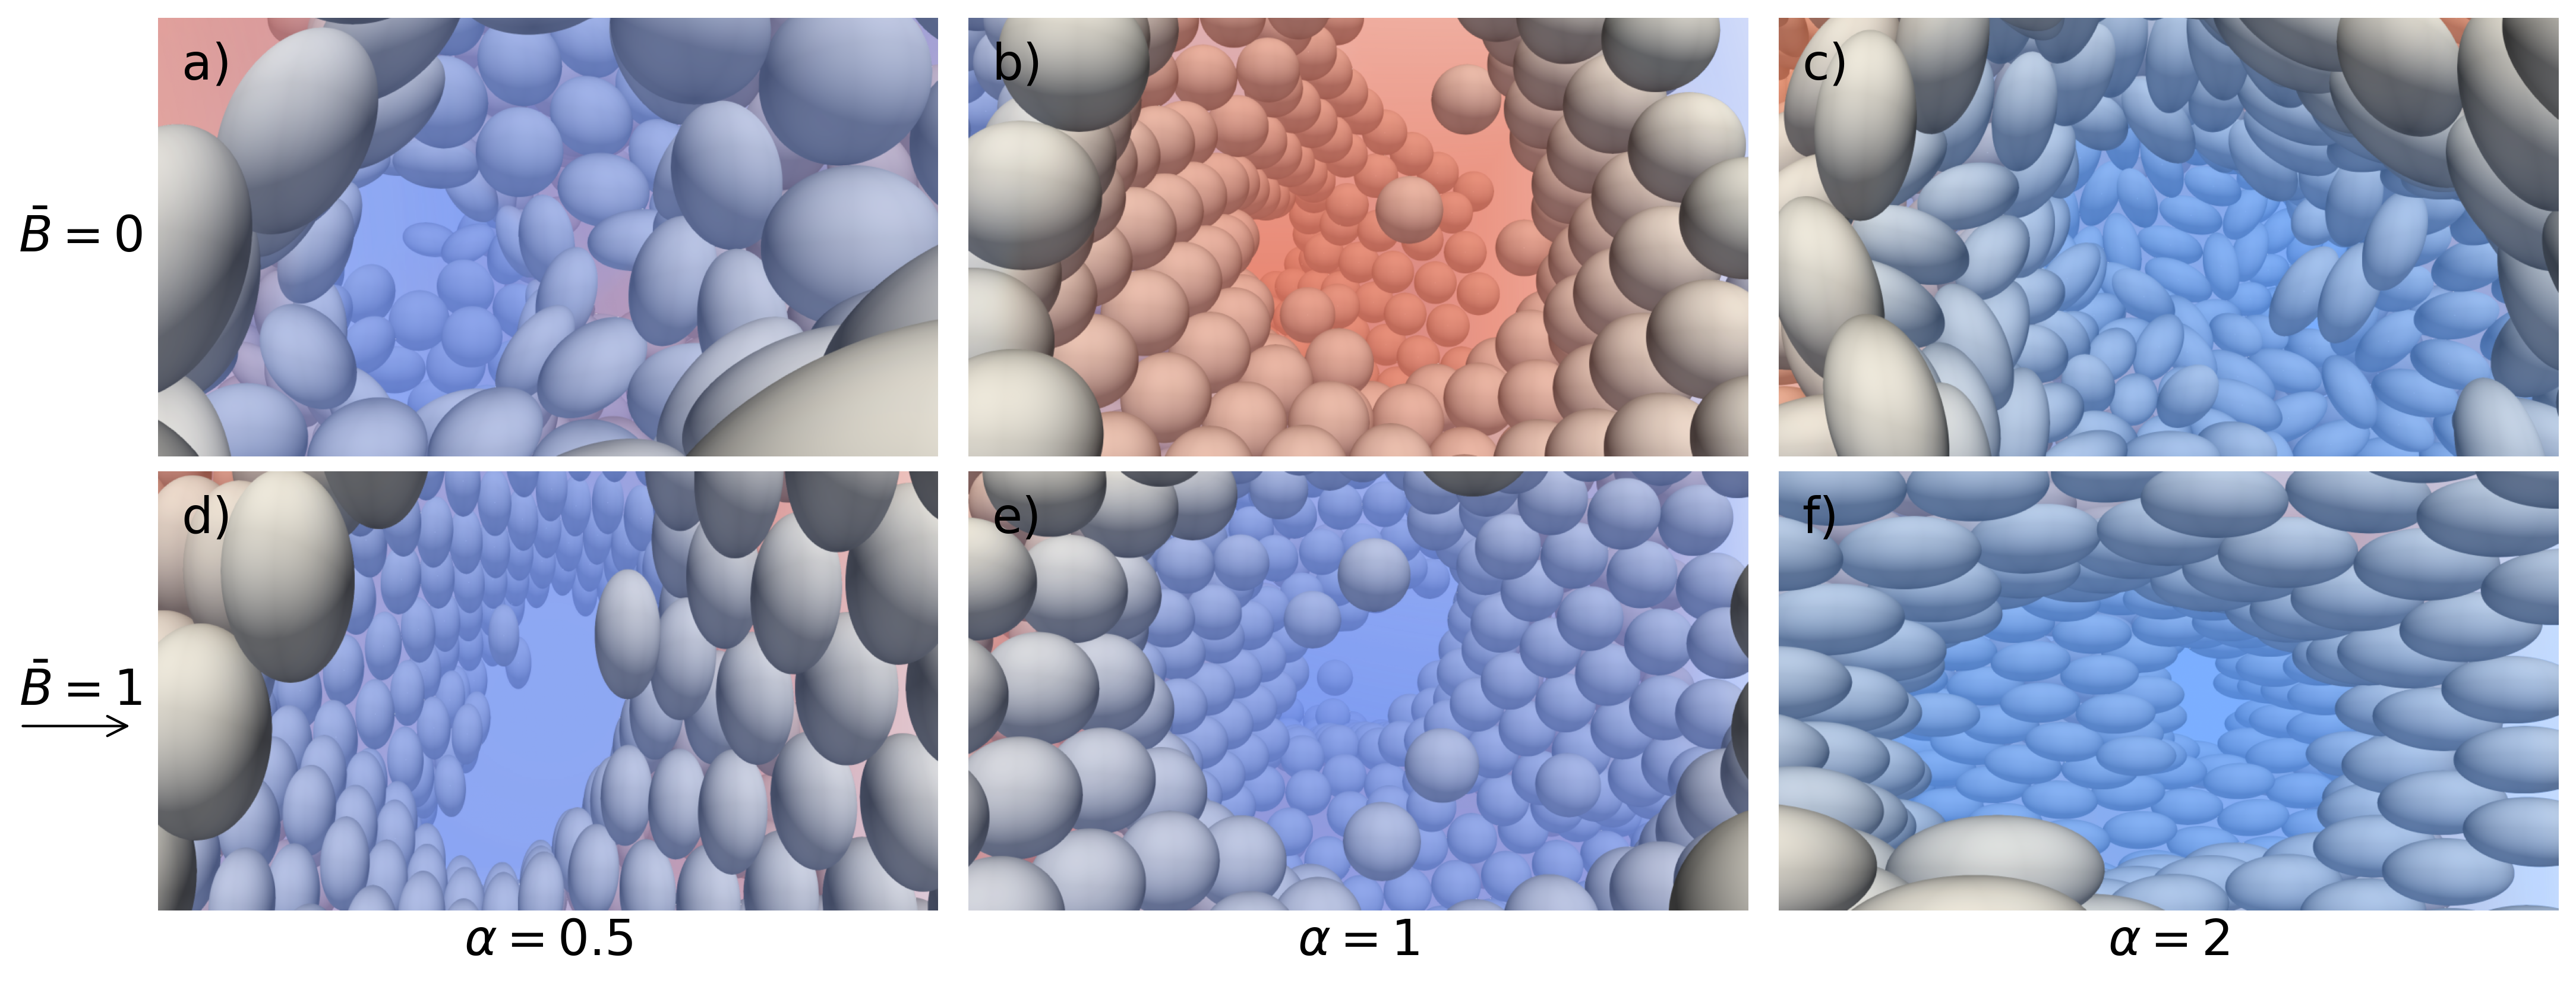
\includegraphics[scale = 0.4]{../figures/results/paper1_5/particle_layer.png}%
\caption{Visualizations of the order parameter $\phi$ for bijels stabilized by oblate (left), spherical (middle) and prolate (right) particles 
         after $10^5$ simulation time steps. The top row shows the structure of bijels formed in the 
         absence of a magnetic field, while the bottom row shows the structure of bijels formed at $\bar{B} = 1$. 
         The direction of the magnetic field is indicated by the arrow.
\label{fig:particle_layer}}%
\end{figure}

We simulated bijel formation following the procedure outlined in Section~\ref{section:sim_setup}, using magnetic particles of varying shape—spherical (\(\alpha = 1\)), oblate (\(\alpha = 0.5\)), 
and prolate (\(\alpha = 2.0\))—at a fixed volume fraction of \(\phi_p = 0.15\). The external magnetic field strength was varied across a range of reduced field values \(\bar{B} = [0, 0.2, 0.5, 1.0]\). 
Snapshots of the final configurations are shown in Fig.~\ref{fig:microstructure_viz}, illustrating the arrangement of particles at the liquid-liquid interface for each shape and field strength. As the 
field strength increases, we observe notable changes in the interfacial particle structure. In particular, the field induces alignment of the particle symmetry axes along the field direction, and this 
orientational ordering appears to promote enhanced local packing within the interfacial monolayer. To quantify this effect, we assess whether the magnetic field leads to increased bond orientational 
order within the particle layer, thereby linking field-induced alignment to changes in monolayer structure.

\subsection{Bond orientational order within the particle layer}

To quantitatively assess the local arrangement of particles at the interface, we compute the ensemble-averaged Steinhardt bond orientational order parameters $q_2$ and $q_6$.
\cite{steinhardt_bond-orientational_1983, lechner_accurate_2008, mickel_shortcomings_2013}. These parameters characterize the local structural ordering by projecting the orientations of neighboring particles 
onto spherical harmonics of degree \(l\), and are defined as


\begin{equation}
q_l(i) = \left( \frac{4\pi}{2l+1} \sum_{m=-l}^{l} \left| \frac{1}{N(i)} \sum_{j=1}^{n(i)} Y_{lm}(\vec{r}_{ij}) \right|^2 \right)^{\frac{1}{2}} ,
\end{equation} 
%\TODO{update formula to the one actually used}

Here, \(n(i)\) denotes the number of nearest neighbors of particle \(i\), \(\vec{r}_{ij}\) is the vector connecting the centers of particles \(i\) and \(j\), and \(m\) is an integer ranging from \(-l\) 
to \(l\) that indexes the spherical harmonic components \(Y_{lm}\). Neighbor lists are typically defined using a fixed cutoff radius around each particle, identifying nearby particles as neighbors. 
We calculate the python package Freud to calculate the bond order parameters and use a Voronoi cell to determine the particle neighborhood rather than the standard distance criterion 
\cite{ramasubramani_freud_2020,mickel_shortcomings_2013}. The Voronoi-based method avoids the need for a predefined cutoff and yields more robust neighbor definitions, particularly in disordered systems. 
Bond orientational order parameters have been widely employed to study structural transitions in colloidal and ceramic systems, including crystallization, nucleation, and glass formation 
\cite{vagberg_glassiness_2011, besseling_three-dimensional_2007, schall_structural_2007, ozawa_jamming_2012}. $q_6$ is most commonly used to identify crystal structures by matching the calculated
values to reference values for specific crystal structures such as fcc or hcp. However, Kapfer et al. pointed out that only using $q_6$ can result in false positives for amorphous systems. \cite{kapfer_jammed_2012}
Mickel et al. identified that $q_2$ vanishes for ordered crystal arrangements and is finite for disordered particle arrangements. \cite{mickel_shortcomings_2013} Therefore we report both to
characterize the particle layer. 

\begin{figure}
\centering
\includegraphics[scale = 0.38]{../figures/results/paper1_5/steinhardt_time.png}%
\caption{Time dependence of the Steinhardt order parameters $q_2$ and $q_4$ for different particles shapes $\alpha$ and at different magnetic field strengths $\bar{B}$. The filled bands around the lines indicate the standard deviation over three independent simulation runs.}
\label{fig:steinhardt_time}%
\end{figure}

Figure~\ref{fig:steinhardt_time} shows the time evolution of the Steinhardt order parameters \(q_2\) and \(q_6\) for all simulated magnetic field strengths and particle shapes. Both parameters begin 
to rise sharply around \(10^4\) timesteps, aligning with the onset of interfacial jamming and the deceleration of domain coarsening previously reported in \cite{karthikeyan_formation_2024}. This increase 
reflects closer packing of particles at the interface, where enhanced local density amplifies the contributions of neighboring particles to the order parameters. The growth in \(q_6\) indicates a 
rise in six-fold orientational order, as also qualitatively seen in the particle arrangements shown in Fig.~\ref{fig:particle_layer}. However, the persistence of finite \(q_2\) values suggests that the 
monolayers remain disordered. Despite visual indications of local order in the 2D interfacial projections, the three-dimensional curvature of the interface causes angular deviations between neighboring 
particle vectors \(\vec{r}_{ij}\), resulting in non-canceling contributions to the \(Y_{2m}(\vec{r}_{ij})\) terms. These results are consistent with previous findings that characterize bijels as two-dimensional 
colloidal glasses embedded within a curved, three-dimensional structure \cite{ching_bijel_2022}.

\begin{figure}
\centering
\includegraphics[scale=0.45]{../figures/results/paper1_5/steinhardt_field.png}%
\caption{Dependence of the Steinhardt order parameter $q_2$ and $q_4$ on the magnetic field $\bar{B}$. The order parameters were computed for the final 
         bijel microstructure after $10^5$ simulation time steps. Errorbars indicate the standard deviation taken over three independent simulation runs.
\label{fig:steinhardt_field}}%
\end{figure}

Figure~\ref{fig:steinhardt_field} presents the variation of the bond orientational order parameters \(q_2\) and \(q_6\) with magnetic field strength for fully arrested bijel structures at \(10^5\) 
timesteps. The consistently finite values of \(q_2\) across all field strengths indicate that the interfacial particle arrangements lack long-range crystalline order, irrespective of whether a magnetic 
field is applied. Notably, \(q_2\) remains largely unaffected by the strength of the applied field. In contrast, \(q_6\), which reflects the degree of six-fold orientational symmetry, varies with both 
particle shape and magnetic field. For spherical particles, \(q_6\) reaches the highest values, while for ellipsoidal particles, the magnitude of \(q_6\) is generally reduced. In the case of oblate 
(disk-like) ellipsoids, \(q_6\) decreases as the magnetic field increases, whereas for prolate (rod-like) ellipsoids, \(q_6\) grows with increasing field strength, though it remains lower than that 
observed for oblate particles. These results suggest that magnetic alignment promotes six-fold ordering in the interfacial monolayer, with the extent of ordering modulated by particle aspect ratio. 
For prolate particles, the elongated shape imposes geometric constraints that suppress perfect six-fold symmetry. Meanwhile, the reduced \(q_6\) for oblate particles under strong fields may be attributed 
to out-of-plane tilting or stacking effects relative to the interface \cite{dabat_mesoscale_2018}. Overall, while the interfacial layers exhibit some degree of six-fold order in two dimensions, the 
non-zero \(q_2\) values confirm that the particle arrangement remains amorphous in three dimensions due to interfacial curvature. This motivates further exploration of how the trends in \(q_6\) with 
field strength relate to changes in the mean and Gaussian curvature of the interface.

\subsection{Curvature of the interface}

Interfacial curvature provides geometric descriptors that complement other measures of bijel morphology and are directly relevant to understanding transport properties in the resulting porous structure.
\cite{reeves_quantitative_2016} The local principal curvatures \(\kappa_1\) and \(\kappa_2\) are obtained as the inverse of the radii of curvature, \(R_1\) and \(R_2\) and are used to calculate
the area averaged mean $H$ and Gaussian $K$ curvatures.

\begin{align}
\langle H \rangle &= \frac{1}{A}\int_A \frac{\kappa_1+\kappa_2}{2} \mathrm{d}A , \\
\langle K \rangle &= \frac{1}{A}\int_A \kappa_1\kappa_2 \mathrm{d}A .
\end{align} 

To compute curvature, we begin by calculating 
the order parameter field \(\phi(\vec{x}) = \rho^{b}(\vec{x}) - \rho^{r}(\vec{x})\), defined as the local density difference between the two fluid components at each lattice site. Since the presence 
of colloidal particles creates voids in the density field, we apply a particle-filling procedure similar to that used in dynamic simulations to fill uncovered grid points. This step iteratively fills 
the lattice nodes occupied by particles using local averaging from surrounding fluid nodes, thereby reconstructing a continuous order parameter field that more accurately represents the interface geometry.
From the completed \(\phi\) field, we extract the bijel interface as the \(\phi = 0\) isosurface using the marching cubes algorithm implemented in the \texttt{scikit-image} library \cite{van2014scikit}. 
We then compute the mean and Gaussian curvatures of the interface using the \texttt{PyVista} package \cite{sullivan2019pyvista}. and are used to compute the Gaussian curvature \(K = \kappa_1 \kappa_2\) and mean curvature \(H = \frac{1}{2}(\kappa_1 + \kappa_2)\) at each mesh vertex.


\begin{figure}
    \centering
\includegraphics[scale=0.5]{../figures/results/paper1_5/curvature_field.png}%
\caption{Plot of the area averaged mean $\langle H \rangle \Sigma^{-1}$ and Gaussian $\langle K \rangle \Sigma^{-2}$ curvature in the left and right 
         respectively. Each plot contains the $\langle H \rangle \Sigma^{-1}$ and $\langle K \rangle \Sigma^{-1}$ at the final timestep averaged across 
         3 runs for particles with $\alpha = 0.5, 1, 2$. We observe that the mean curvature does not demonstrate any trends, while the Gaussian curvature 
         shows a reduction as the magnetic field strength is increased for ellipsoidal particles.}
\label{fig:curvature_field}%
\end{figure}

Figure~\ref{fig:curvature_field} shows the dependence of the area-normalized mean and Gaussian curvature,\(\langle H \Sigma^{-1} \rangle\) and \(\langle K \Sigma^{-2} \rangle\) respectively, on the 
applied magnetic field strength. As expected for systems with equal fluid volume fractions and neutrally wetting particles, the mean curvature remains close to zero across all field strengths and shows 
no significant field dependence, reflecting the absence of a preferred direction for interfacial bending \cite{jinnai_interfacial_2001}. In contrast, the Gaussian curvature exhibits a clear trend for 
ellipsoidal particles, becoming increasingly negative with higher magnetic field strength. This indicates that the interface adopts a more pronounced saddle-like geometry as the field strengthens.
Previous work has shown that bijels formed with smaller stabilizing particles, such as nanoparticles, exhibit more negative Gaussian curvature due to their enhanced ability to conform to curved interfacial 
geometries \cite{reeves_quantitative_2016}. This behavior is attributed to their smaller cross-sectional area, which introduces minimal disruption to the hyperbolic character of the interface. Consistent 
with these findings, our zero-field results show that ellipsoidal particles produce less negative Gaussian curvature than spheres. Specifically, the oblate and prolate particles used here have approximately 
60\% and 30\% larger cross-sectional areas, respectively, compared to spheres of the same volume. However, under increasing magnetic field strength, these anisotropic particles align with the field direction, 
effectively reducing their projected area at the interface. This reorientation enables the interface to adopt more negatively curved geometries, explaining the observed decrease in 
\(\langle K \Sigma^{-2} \rangle\) with field strength. These curvature changes suggest corresponding shifts in the topology of the bijel structure, motivating a closer examination of its topological features.


\subsection{Topology of the emulsion microstructure}

Domain size is one of the most widely used metrics for characterizing coarsening in emulsions. Common approaches to determine domain size include calculating the moments or identifying peaks in the structure 
factor, which are often used to detect dynamic scaling regimes \cite{kendon_inertial_2001}. However, these definitions do not always yield an accurate representation of the true domain dimensions 
\cite{karthikeyan_formation_2024}, and domain size alone does not fully capture morphological variations in bijels under different processing conditions \cite{reeves_quantitative_2016}. The Gauss-Bonet
theorem connects the curvature of a surface to its topology through parameters such as the genus($g$) which can be thought of as the number of holes in a surface. Spheres and torii have a genus of 0 and 1 respectively. 
In this context, we also calculate the number of handles($h$) defined as channels through the volume and voids($v$) which characterize the number of disconnected cavities or loops. The relation between genus \(g\), 
number of handles \(h\), and number of voids \(v\) is thus expressed by \cite{chan_channel_2012}

\begin{equation}
g = h - v .
\end{equation} 

The genus is related to the Euler-Poincar\'e characteristic \(\chi\) of the surface, i.e., 

\begin{equation}\label{eq:genus}
g = 1 - \frac{\chi}{2} .
\end{equation} 

To compute the Euler-Poincaré characteristic, we used the \texttt{skimage.measure.euler\_number} function from the scikit-image library. In this implementation, the Euler characteristic is defined as the 
number of objects plus the number of holes minus the number of loops, effectively incorporating the factor of 1/2 in Eq.~\ref{eq:genus} into the returned value. As a result, the genus \(g\) was determined 
by subtracting the Euler characteristic from the total number of connected objects. The number of voids was calculated using \texttt{skimage.measure.label}, also from scikit-image, by identifying and 
excluding all regions connected to the boundary of the simulation volume. The number of handles was then obtained by applying Eq.~\ref{eq:genus}.

\begin{figure}
    \centering
\includegraphics[scale=0.45]{../figures/results/paper1_5/handles_time.png}%
\caption{Time dependence of the number of channels for different particle shapes $\alpha$ and at different magnetic field strength $\bar{B}$. 
         The bands around the lines indicate the standard deviation taken over three independent simulation results. The number of channels roughly 
         follows a power law behavior $\sim t^{-3/2}$ which suggests that it is inversely proportional to the characteristic domain size $L \sim t^{3/2}$.
\label{fig:handles_time}}%
\end{figure}

The temporal evolution of the number of handles—interpretable as the number of continuous channels through the volume—is presented in Fig.~\ref{fig:handles_time}. This measure provides insight 
into coarsening dynamics, particularly the occurrence of coalescence and pinch-off events. Across all simulations, regardless of particle shape or magnetic field strength, the number of channels 
decreases over time following a similar trend. During the coarsening phase, this decrease closely follows a power law relationship \(h \sim t^{-2/3}\), which is consistent with the known scaling 
law for the domain size \(L \sim t^{2/3}\). This inverse relationship suggests that the number of channels is proportional to the inverse of the characteristic domain size. 
Neither particle anisotropy nor magnetic field strength significantly alters this dynamic scaling behavior during the early stages of coarsening. However, once jamming begins, the reduction in the 
number of channels slows down, though it does not stop entirely. This behavior aligns with earlier findings by Harting and collaborators \cite{gunther_timescales_2014}, which identified multiple 
timescales governing bijel formation. Additionally, we observe that higher magnetic field strengths tend to delay the onset of jamming, consistent with previous observations of reduced coarsening 
rates under such conditions \cite{karthikeyan_formation_2024}.
Following jamming, the final number of channels varies with particle shape and magnetic field strength, likely reflecting the specific domain morphology present at the onset of structural arrest. 
Some regions may already be immobilized while others remain dynamic, contributing to the slow, continued reduction in channel number. Nevertheless, our results do not reveal a clear or systematic 
dependence of the final channel count on particle anisotropy or field strength.

%\TODO{need some comments on coarsening kinetics here and literature references, e.g., comparing to number of droplets over time}

To characterize topological changes in the bijel structure, we compute the channel size distribution (CSD) following the method developed by Chan and Thornton \cite{chan_channel_2012}. This approach begins 
with the construction of a signed distance field from the order parameter \(\phi\), which is reinitialized using the level set algorithm described by Sussman et al.~\cite{sussman_level_1994, chan_channel_2012}. 
The resulting distance transform is smoothed using a boxcar-averaging stencil with periodic boundary conditions to reduce numerical artifacts arising from grid discretization \cite{chan_channel_2012}. 
From the smoothed distance field, a series of isosurfaces are extracted at normalized distances \(\bar{r} = r \cdot \Sigma\), where \(\Sigma\) is the specific interfacial area. The number of handles is computed 
for each of these isodistance surfaces. A decrease in the number of handles with increasing distance from the interface reflects the pinch-off of channels, providing insight into the evolving connectivity of the 
microstructure. The channel size distribution is then obtained from the negative derivative of the handle count with respect to \(\bar{r}\), yielding a statistical measure of channel sizes as a function of 
distance from the interface.

\begin{equation}
f(r) = - \frac{d h(r)}{dr} .
\end{equation}

\begin{figure}
    \centering
\includegraphics[scale = 0.4]{../figures/results/paper1_5/CSD.png}%
\caption{Channel size distribution (CSD) in bijels stabilized by oblate ($\alpha=0.5$), spherical ($\alpha=1.0$), and prolate ($\alpha=2.0$) particles. 
         The channel size distribution was obtained as the negative derivative of the number of handles in isodistance structures of the Euclidean distance 
         transform of the order parameter field. The negative values are due to numerical artifacts when calculating the number of handles as a function of 
         isodistance from the interface.}
\label{fig:CSD}%
\end{figure}

Figure~\ref{fig:CSD} presents the channel size distribution (CSD) for bijels formed with three different particle shapes under varying magnetic field strengths. Minor negative values appear in 
the distribution due to numerical artifacts associated with computing the number of handles as a function of distance from the interface. Overall, we do not observe any consistent or systematic 
trends related to particle shape or field strength. The channel sizes span a broad range, extending up to approximately \(0.6 \cdot \Sigma^{-1}\), which corresponds to about 20\% of the total system 
size. This wide distribution reflects the structural complexity of bijel morphologies, which include both broad channels and narrow regions where opposing interfaces are separated by distances 
comparable to the particle size. Although previous results indicated anisotropic domain sizes, suggesting the possibility of a bimodal channel distribution, such a feature is not evident in the 
present data. It is possible that a larger simulation domain would be required to resolve such effects more clearly, which could be explored in future work.

\begin{figure}
\centering
\includegraphics[scale = 0.6]{../figures/results/paper1_5/channel_size_field.png}%
\caption{Average channel size $L_c$ for different particle shapes $\alpha$ and at different magnetic field strength $\bar{B}$. The average channel size was calculated from the channel size distribution shown in Fig.~\ref{fig:CSD}. Errorbars indicate the standard deviation taken over three independent simulation runs.
\label{fig:channel_size_field}}%
\end{figure}

To relate the channel size distribution (CSD) to previous estimates of the characteristic domain size, we calculated the average channel size \(L_c\), shown in Fig.~\ref{fig:channel_size_field}. For 
systems stabilized by spherical particles, we observe relatively large error bars, representing the standard deviation across three independent simulations. This variability is likely due to the 
sensitivity of the final microstructure to the initial particle arrangement, which can influence the timing of jamming and the pathways available for coarsening—as reflected in the time evolution of 
the number of channels. In contrast, for anisotropic particles, the average channel size increases with magnetic field strength. This trend, along with the overall scale of \(L_c\), is in good agreement 
with previous domain size measurements based on structure factor moments (see Fig. 4 in Ref.~\citenum{karthikeyan_formation_2024}). Thus, identifying channel sizes through topological analysis of 
isodistance surfaces offers an alternative and complementary approach to quantifying domain size in bicontinuous emulsions. Moreover, this method reveals additional insights into the coarsening dynamics 
that are not captured by traditional geometric or structural metrics.


\section{Conclusions\label{conclusions}}

We analyzed the structural properties of bijels stabilized by magnetic ellipsoidal particles using data from Lattice Boltzmann–Molecular Dynamics simulations of binary mixtures containing oblate, 
spherical, and prolate magnetic particles across varying magnetic field strengths. Structural characterization included bond orientational order via Steinhardt parameters, interfacial mean and 
Gaussian curvature, and topological features of the emulsion morphology. In the jammed state, particle layers showed evidence of six-fold ordering but lacked crystalline symmetry in 3D due to 
interfacial curvature. We also found that anisotropic particles induce greater Gaussian curvature than spheres, while increasing magnetic field strength reduces Gaussian curvature—suggesting that 
magnetic alignment enhances the hyperbolic nature of interfaces, promoting more robust bijel formation with anisotropic particles.

To track coarsening, we quantified topological evolution through the number of handles, which reflects the count of channels in the bicontinuous structure. This number decreases over time following a 
power-law trend inversely proportional to domain size. The decay rate slows after jamming, consistent with prior findings \cite{gunther_timescales_2014, karthikeyan_formation_2024}. We further 
extracted channel size distributions (CSDs) from isodistance surfaces of the level set reinitialization \cite{chan_channel_2012}, revealing a broad range of channel sizes without systematic 
changes across magnetic field strengths. However, the average channel size from the CSD agrees with previous domain size measurements.

Our results bridge multiple aspects of bijel morphology: interfacial particle packing connects to local curvature, while global topological features relate to coarsening events such as domain 
coalescence and channel pinch-off. This study extends previous curvature analyses by Reeves et al.~\cite{reeves_quantitative_2016} and CSD measurements in Cahn-Hilliard systems by Chan and 
Thornton \cite{chan_channel_2012}, offering a more detailed view than conventional global metrics like domain size. These structural descriptors are also relevant for applications: interfacial 
particle order correlates with yield stress in emulsions \cite{besseling_three-dimensional_2007, schall_structural_2007, madivala_exploiting_2009, vagberg_glassiness_2011, kaganyuk_shear-induced_2020}, 
and interface curvature affects cell adhesion and reaction kinetics in energy systems \cite{xiong_porosity_2024, shojaei_minimal_2022}.
Understanding how these properties depend on formulation and processing conditions is key for bijel design. By analyzing independent simulations with varied initial conditions, we also captured 
statistical variation in features like channel size and its distribution. These insights lay the groundwork for systematic tuning of bijel fabrication. In particular, magnetic ellipsoidal particles 
offer promising avenues for controlled modulation of interfacial structure and domain morphology.

\chapter{Structural response of bijels under magnetic fields}
\label{chapter:aim2}
Previous work demonstrated that applying electric fields to silica-stabilized emulsion droplets 
caused particle stabilizers to unjam and then rejam, locking the emulsion in a new morphology. 
\cite{cui_stabilizing_2013} Considering the potential applications of an already synthesized porous 
material with tunable microstructure, the second part of this work will explore using magnetic fields 
to manipulate bijels after synthesis. \cite{vanoli_bijels_2022, cha_bicontinuous_2019} Bijels simulated 
under no field had a constant magnetic in the z direction of strength $\Bar{B} = 0, 0.2, 0.5, 1$ with their
 microstructure and particle order analyzed.

Underlying mechanism being rearrangement of particles on the interface in response to magnetic field, or 
unjamming and rejamming characterized by a change in the number of bonded neighbors. Explains behaviour 
seen in differences in the system above and below the isotropic to nematic transition? 

\begin{figure}
    \centering
    \includegraphics[scale = 0.5]{figures/results/paper2/domain_size.png}
    \caption{Left plot shows the average domain size $(L_1)$ in markers and the nematic order parameter $(S)$ in lines versus time. Right plot shows the same data rescaled over $t_{iso \rightarrow nematic}$.}
    \label{fig:P2_domain_scaling}
\end{figure}

In this system, the mechanism of microstructure modification after formation is expected to be due to magnetic 
field driven particle ordering changes. Figure \ref{fig:P2_domain_scaling} demonstrates that the average domain 
size $(L_1)$ does not change significantly with the applied field, with a slight increase of about $\approx 0.3 L/R$, 
noted to be within error. However, clues into the underlying mechanics are visible when examining the nematic order 
parameter lines overlaid on the domain size markers. At $\Bar{B} = 0.2$, the domain size change corresponds with the 
nematic order parameter change, indicating a direct link between domain size change and particle ordering. 
At $\Bar{B} > 0.2$, a gap appears between the domain size change and the nematic order parameter change, suggesting 
steric effects influence the rate of bijel microstructure change. The timescales of these rearrangements may also 
impact the observed microstructure changes, which can be characterized by the domain size change over time rescaled 
by a characteristic timescale.

A naive guess as to the dominating timescale of the response would be the isotropic to nematic time of the 
system or when $S \geq 0.3$. The right plot of Figure \ref{fig:P2_domain_scaling} demonstrates the time 
evolution of the system when rescaling time with the isotropic to nematic transition time,
 $t_{iso \rightarrow nematic}$. From this plot, it can be seen that application of the field 
 causes collapse of domain size changes at different field strengths on top of one another, 
 showing that this naive guess is a correct one. The changes in domain size at with no applied
  field can be attributed to the reordering of particles at the interface, leading to coarsening 
  at long time scales consistent with what Gunther et al. observed. \cite{gunther_timescales_2014}

\begin{figure}
    \centering
    \includegraphics[scale = 0.5]{figures/results/paper2/domain_size_aniso.png}
    \caption{Plots of the perpendicular $(L_{\perp})$ and parallel $(L_{\parallel})$ domain sizes over time rescaled over $t_{iso \rightarrow nematic}$}
    \label{fig:P2_domain_aniso}
\end{figure}

In the previous section, even if the average domain size did not change much, there was domain size anisotropy 
found upon application of the field. This observation and trends seen remains true when applying the field 
after formation as can be observed in \ref{fig:P2_domain_aniso}. Time was again rescaled with the isotropic 
to nematic transition time for each system, demonstrating that the timescale of response is controlled using 
this timescale, and is independent from field strength. The domain size change observed appears to be about $1 L/R$ 
less than what can be found when applying the same field size during bijel synthesis as the increase in domain size 
for $L_{parallel}$ for prolate particles is $\approx 2 L/R$ which is $50 \%$ lower than what was found. This 
indicates that microstructure control after synthesis is not as effective. This might be due to steric effects 
being much stronger after synthesis, limiting how much particles can move or tilt before rejamming. Despite 
this, the domain size change found is well within what has been seen to be effective in the literature, 
indicating that magnetic field enabled in-situ microstructure modifications can be utilized within bijels. 
\cite{cha_bicontinuous_2019, khan_nanostructured_2022, vanoli_bijels_2022}

\begin{figure}
    \centering
    \includegraphics[scale = 0.5]{figures/results/paper2/interface_angle.png}
    \caption{Plots of the average angle between the particle dipole moment and interface normal $(\psi)$ over time. While there are minor changes in for the oblate particles, these are not as significant as the ordering of particles to the field.}
    \label{fig:P2_interface_angle}
\end{figure}

To determine if the interface follows the orientation of the particles, the average angle between the 
particle symmetry axis and the interface normal $(\psi)$ was plotted against time rescaled by 
$t_{iso \rightarrow nematic}$ in Figure \ref{fig:P2_interface_angle}. From ths plot, it can be 
observed that upon application of the magnetic field, the particle tilts out of the interface at 
an equal normalized rate. However, the angle reached before the particles begin returning to their 
equilibrium configuration is magnetic field strength dependent, suggesting that the degree of 
microstructure changed observed might be dependent on how much the particle tilts away from its 
equilibrium position. At non-equilibrium particle tilts, there is more leeway for coarsening to 
occur before rejamming occurs, resulting in larger microstructural differences. 

Future work will more closely examine the role of the particles in observed microstructure changes 
by calculating the average angle between the particle symmetry axis and the interface normal. 
In addition, the impact of initial order of the particle monolayer on the degree of microstructure 
change observed will be characterized. This will be accomplished by using bijels that have been 
simulated under magnetic fields and changing the applied field. Example conditions would be a bijel 
being simulated under a field strength of $\Bar{B} = 0.2$ and increasing the applied field to $\Bar{B} = 1$ 
or switching off the applied field. Based on the findings so far it is predicted that initial particle order 
and microstructure change are inversely correlated. Additionally, the timescales of these microstructure 
changes will be investigated. When switching a field on, there are magnetic field, steric and interfacial 
forces that govern the dynamics. However, when reducing the field strength, the magnetic field derived force 
isn't present, resulting in steric and interfacial forces playing a significant role. These differences can 
be examined by investigating the timescales the observed response occurs at, as well as the particle 
properties over time.

% \textcolor{blue}{Still needs additional explanation of how using templates made under fields and decreasing and increasing field strengths will change results}


\chapter{Rheological response of bijels under magnetic fields}
\label{chapter:aim3}
% Previous work into shearing bijels have demonstrated how particles prefer to move in the direction of shear and if strong enough, even detach from the interface. \cite{bonaccorso_shear_2020} It has also been shown how at curved interfaces, ellipsoidal particles  

In many of the manufacturing techniques outlined for continuous bijel production such as STrIPS, the rheological properties are essential in ensuring that the casting mixture remains processable. However, past work with ferrofluids and magnetic emulsions have showed how the rheological properties vary drastically as a function of the field strength. Bijels themselves have complex rheological properties stemming from the removal of particles from the interface if too much shear is applied. Therefore, avenues of exploration here would be how the rheological properties of bijels change under the influence of fields in response to an applied shear. One of the questions that will be investigated in particular will be how shear changes the orientation of the particles on the interface, the interfacial coverage of particles and if there is anisotropy in the viscosity during the application of a field owing to the orientation of particles towards the field.

First, a shear capillary number is defined as $Ca_s = \frac{\eta_{f} \dot{\gamma} L_{1}}{\sigma}$ where $\dot{\gamma} = \frac{u_{LE}}{L_x}$ is the strain rate and $L_1$ is the average domain size. \cite{frijters_effects_2012, yang_capillary_2022} In the literature, $Ca_s$ has been between between 0.04 and 0.16. However, the box size in these simulations were smaller, meaning that these capillary number ranges would exceed the maximum mach number the model allows if this same range were used $(Ma \leq 0.03)$. To accommodate this limitation the largest capillary number used will be $Ca_s = 10^-5$ which correspond to a maximum of $Ma \approx 0.002$. $Ca_s = 10^-6,  10^-7$ will also be used to demonstrate how the bijels respond to shear of varying strengths. As all particles used have only hard-sphere type interactions, it is expected that the behaviour seen should mimic 2D colloidal glasses percolating in 3D space, akin to what Ching and Mohraz saw, with an additional dependence on -the direction of shear. This would predict the discovery of particle monolayer dependent elasticity and yield stress along with shear thinning behaviour as a function of strain rate. 

To verify these predictions, bijel microstructure will be defined using four processing histories; The first is of a bijel simulated under a $\Bar{B} = 1$ magnetic field strength, the second is a bijel stimulated under no field, followed by the application of a $\Bar{B} = 1$ field after jamming, the third is a bijel simulated under no field, while the final microstructure is a bijel simulated under $\Bar{B} = 1$ magnetic field, followed by switching the field off after jamming. This gives insight into the impact of processing history on the shear properties of a bijel, in addition to the microstructural and colloidal insights gained. Based on the results in Bonaccorso et al., there should be shear driven and shear rate dependent elongation of the domains in the direction parallel to the applied shear which in this system will be seen as a reduction in $L_{\perp}$ and an increase in $L_{\parallel}$. \cite{bonaccorso_shear_2020} The microstructure anisotropy will also be a factor in the viscosity results, as larger domains are more permeable than smaller ones, meaning that bijels where $L_{\perp} > L_{\parallel}$ should see less of the domain elongation effects shown in Bonaccorso et al. as the permeability of the bijels rises with larger domain size. \cite{bonaccorso_shear_2020}

It is also expected that the effective viscosity will be different between the four microstructures dependent upon the degree of nematic ordering and microstructural anisotropy of the bijel. Nematic ordering of the particles will be mimic shear banding in colloidal suspensions, resulting in a lowered effective viscosity compared to bijels without nematically ordered particles. \cite{xu_relation_2013, vermant_flow-induced_2005} Tracking of the proportion of particles on the interface will also yield insight into how the packing of the particles affects the rate at which particles will get ejected from the interface. Systems with a larger $\eta_{eff}$ are predicted to have the largest domains, largest difference between initial and final particle order and lowest number of particles left on the interface once steady state has been established. 


\chapter{Final remarks}
\label{chapter:final_remarks}
\section{Conclusion}

Owing to their high surface area to volume ratio, porous materials are seeing a surge in popularity in applications
such as catalysis, battery electrodes and pharmaceuticals. Given their wide variety of applications, identifying 
fabrication techniques that allow access to the various pore length scales is of interest. One such synthesis technique
is emulsion templating which offers a wide variety of accessible microstructures, addition of stimuli response and 
large number of possible systems that can be fabricated. A microstructure that can be fabricated from emulsion templates
is the bicontinuous interfacially jammed emulsion gel (bijel). 

Bijels are normally fabricated using Thermally Induced Phase Separation (TIPS). However, TIPS does not allow for continuous
fabrication of bijels. More recent fabrication techniques such as Solvent Transfer Induced Phase Separation (STrIPS) and 
Vapor Induced Phase Separation (VIPS) allow for continuous fabrication and access to various microstructures. Both techniques
require modifications to the initial emulsion mixture to facilitate microstructure adjustments, which affect the final rheological
properties of the system. Decoupling the microstructure and the casting mixture of the bijel would allow for greater flexibility
in the synthesis of the material.

Stimuli response has been used before to modify the microstructure of particle stabilized emulsions. Magnetic fields offer
targeted material response and low applied field strengths necessary for response. Past work investigating the effect of magnetic
stimuli on bijels stabilized with spherical particles yielded little microstructure change. However, anisotropic particles have
also been used to stabilize bijels. Anisotropic particles at interfaces under magnetic fields have been shown to tilt out of 
interfaces. These effects have yet to be captured in bijels stabilized by ellipsoidal particles under magnetic fields.
This study addresses this knowledge gap using a hybrid Molecular-Dynamics multicomponent method Lattice Boltzmann Method.
We split this work into three aims; Aim 1 addressed the microstructure obtained when applying a magnetic field of various strengths 
onto bijels stabilized by ellipsoidal particles, compared to bijels stabilized wih spherical particles. Aim 2 addressed the 
structural response of bijels stabilized by ellipsoidal particles and analyzes the effect of initial order of the particle monolayer
on the structural response observed. Aim 3 addressed the constant shear response of bijels stabilized by ellipsoidal particles
with pre-existing particle order and under magnetic fields.

In Aim 1, bijels stabilized with spherical particles do not respond to the application of a magnetic field. However, bijels stabilized
with ellipsoidal particles have an increase in the average domain size by 3 \%. The microstructure also becomes anisotropic, 
characterized as a change in the directional tortuosity and distribution of channel widths as a function of the distance from the 
interface. The curvature also becomes more negative as the applied field strength is increased. The microstructure anisotropy is caused
by direction specific jamming of the particle monolayer originating from particle ordering to the magnetic field.

When investigating the particle monolayer, the orientational order changes as a function of the applied field strength and has particle
morphology specific time evolution. The interface angle was also characterized and shown to have magnetic field dependence, although
this was attributed to the orientational ordering of the particles on the interface. When analyzing the ordering of particles on the
interface, disc-like particles see lowered local ordering as the magnetic field strength is increased while rod-like particles see
greater local ordering. These properties are attributed to how those particle morphologies prefer to orient themselves at interfaces
to one another, with disc like particles preferring to stack while rod like particles order side to side or end to end.

In Aim 2

In Aim 3

\section{Future work}

This work utilized 2 ellipsoidal particle geometries chosen for comparisons to previous literature using this 
particle geometry. Particles based on cellulose nanocrystals or graphene nanoplates are now in use to fabricate
particle stabilized emulsions.These particles have also been shown to have capillary bridging and particle stacking,
not seen in the particles used in this work. These particles in bulk have been shown to have some intrinsic ordering
that can be predicted using onsager theory. An investigation into how using rods or plate like particles would be 
instructive in identifying if onsager theory can be used in bijel formation and its link to bijel microstructure. 
\textcolor{blue}{https://doi.org/10.1039/D1SM00367D}

Colloidal systems made with cohesive and soft particles have been shown in the literature to have different glass 
transition points and rheological behavior from their hard sphere counterparts. In bijels, cohesive particles in 
particular have been suggested as a means to create "armored" bijels to improve their performance in catalytic materials, 
allowing higher flow rates to be used. Investigations into soft particles are of interest in biomedical engineering 
applications, with newly developed nanogels and hydrogels being suggested as drug carriers or vectors for stimuli 
response through temperature or pH. LBM methods that implement the immersed boundary method can be used to model soft
particles with a DLVO potential used to model electrostatics between particles. \textcolor{blue}{https://doi.org/10.1039/D3SM01648J}

Another avenue of exploration would be the use of gradient or rotating magnetic fields in place of the constant magnetic 
fields used here. One study on bijel microstructure showed that a gradient in the particle volume fraction can be used to 
create a gradient in the eventual domain size. A gradient field may be able to generate a gradient in the nematic order 
parameter, affecting the particle packing of the bijel at different heights and varying the pore size as a function of 
height in the field gradient direction. In a ferrofluid or solution of magnetic colloids, a rotating field can assemble 
particles into chains or rings. In the context of bijel structural response, this can be used to tune bijel microstructure 
as this process can control the unjamming and rejamming of the particle monolayer, allowing for greater control over the 
resulting bijel microstructure than a constant field would have. In these simulations, the frequency of rotation would 
likely need to be tuned based upon how quickly particles respond to field in the bijel.


% Extensions to this work can be accomplished by investigating the effect of applying a magnetic field on the bijel 
% while under shear. Ferrofluid models that predict bingham plastic like flows, $\frac{\eta}{eta_{f}} = 1 + \frac{Mn^{*}(\phi_p)}{Mn}$, 
% have been developed and defined using the Mason number, $Mn = \frac{8\eta_{f} \dot{\gamma}}{\mu_{0} \mu_{f} \beta^{2} H_0^2}$. 
% \textcolor{blue}{https://doi.org/10.1122/1.4935850, https://linkinghub.elsevier.com/retrieve/pii/S1359029405000385} 

\section{Acknowledgments}

The author acknowledges Dr. Ulf Schiller and the members of the Schiller and Kuksenok groups for the discussions on 
the characterization and computational techniques used in this work. This work is supported by the US National Science 
Foundation under award numbers DMR-1944942 and OIA-2131996. Any opinions, findings, conclusions, or recommendations 
expressed in this material are those of the author(s) and do not necessarily reflect those of the National Science 
Foundation.  

Clemson University is acknowledged for generous allotment of compute time on Palmetto cluster. This research used the 
Delta advanced computing and data resource which is supported by the National Science Foundation (award OAC 2005572) 
and the State of Illinois. Delta is a joint effort of the University of Illinois Urbana-Champaign and its National 
Center for Supercomputing Applications. 

This work used Delta at the University of Illinois Urbana Champaign through allocation PHY220131 from the Advanced 
Cyberinfrastructure Coordination Ecosystem: Services $\&$ Support (ACCESS) program, which is supported by National 
Science Foundation grants 2138259, 2138286, 2138307, 2137603, and 2138296. 


\newpage

\chapter{Figure reproduction licenses}
\section{License numbers}

\begin{itemize}
    \item Continuous Fabrication of Hierarchical and Asymmetric Bijel Microparticles, 
    Fibers, and Membranes by Solvent Transfer‐Induced Phase Separation (STRIPS): 5913140219015
    \item Scalable synthesis of gyroid-inspired freestanding three-dimensional graphene architectures: 1548092-1
    \item State diagram for particle stabilized emulsions. [Soft Matter, 2015,11, 8393-8403]: 1551968-1
    \item Scalable Manufacturing of Hierarchical Biphasic Bicontinuous Structures via Vaporization-Induced 
    Phase Separation (VIPS) [Materials Letters 2020, 2, 5, 524-530]: "Reprinted (adapted) with permission from 
    {COMPLETE REFERENCE CITATION}. Copyright {YEAR} American Chemical Society."
    \item Modulation of Cellulose Nanocrystals Amphiphilic Properties to Stabilize Oil/Water Interface 
    [Biomacromolecules 2016, 17, 5, 1748–1756]: "Reprinted (adapted) with permission from 
    {COMPLETE REFERENCE CITATION}. Copyright {YEAR} American Chemical Society."
    \item Dextran-Based Nanoparticles to Formulate pH-Responsive Pickering Emulsions: A Fully Degradable 
    Vector at a Day Scale [Biomacromolecules 2020, 21, 12, 5358–5368]: "Reprinted (adapted) with permission from 
    {COMPLETE REFERENCE CITATION}. Copyright {YEAR} American Chemical Society."
    \item Stable emulsions with thermally responsive microstructure and rheology using poly(ethylene oxide) star 
    polymers as emulsifiers [Journal of Colloid and Interface Science, 2013, 394, 284-292]: 5921030909190
    \item Magnetophoresis of Magnetic Pickering Emulsions Under Low Field Gradient: Macroscopic and Microscopic 
    Motion [Langmuir 2021, 37, 5, 1811–1822]: "Reprinted (adapted) with permission from 
    {COMPLETE REFERENCE CITATION}. Copyright {YEAR} American Chemical Society."
    \item Influence of magnetic field on the orientation of anisotropic magnetic particles at liquid interfaces 
    [Phys Chem Chem Phys 2014, 16, 47, 26051-26058]: 1551970-1
    \item Pickering Emulsions with Controllable Stability [Langmuir, 2005, 21, 6, 2158-2162]: "Reprinted (adapted) with permission from 
    {COMPLETE REFERENCE CITATION}. Copyright {YEAR} American Chemical Society."
    \item Bijels Containing Magnetic Particles: A Simulation Study [Langmuir, 2010, 26, 11, 7928-7936]: 
    "Reprinted (adapted) with permission from {COMPLETE REFERENCE CITATION}. Copyright {YEAR} 
    American Chemical Society."
    \item Numerical simulations of particulate suspensions via a discretized Boltzmann equation. Part 2. Numerical results
    \item Aerobijels: Ultralight Carbon Monoliths from Cocontinuous Emulsions 
    [Adv. Funct. Mater. 2020, 30, 1908383]: 5921080017718
    \item Hierarchical assemblies of superparamagnetic colloids in 
    time-varying magnetic fields [Soft Matter. 17, 5, 1120-1155]: 1552854-1
\end{itemize}

\newpage

\bibliographystyle{myphpf}
\bibliography{references}

\end{document}